%%%%%%%%%%%%%%%%%%%%%%%%%%%%%%%%%%%%%%%%%%%%%%%%%%%%%%%%%%%%%%%%%%%%%%
% Template for a UBC-compliant dissertation
% At the minimum, you will need to change the information found
% after the "Document meta-data"
%
%!TEX TS-program = pdflatex
%!TEX encoding = UTF-8 Unicode

%% The ubcdiss class provides several options:
%%   gpscopy (aka fogscopy)
%%       set parameters to exactly how GPS specifies
%%         * single-sided
%%         * page-numbering starts from title page
%%         * the lists of figures and tables have each entry prefixed
%%           with 'Figure' or 'Table'
%%       This can be tested by `\ifgpscopy ... \else ... \fi'
%%   10pt, 11pt, 12pt
%%       set default font size
%%   oneside, twoside
%%       whether to format for single-sided or double-sided printing
%%   balanced
%%       when double-sided, ensure page content is centred
%%       rather than slightly offset (the default)
%%   singlespacing, onehalfspacing, doublespacing
%%       set default inter-line text spacing; the ubcdiss class
%%       provides \textspacing to revert to this configured spacing
%%   draft
%%       disable more intensive processing, such as including
%%       graphics, etc.
%%

% For submission to GPS
%\documentclass[gpscopy,onehalfspacing,11pt]{ubcdiss}

\pdfminorversion=6
% For your own copies (looks nicer)
\documentclass[balanced,twoside,11pt]{ubcdiss}

%%%%%%%%%%%%%%%%%%%%%%%%%%%%%%%%%%%%%%%%%%%%%%%%%%%%%%%%%%%%%%%%%%%%%%
%%%%%%%%%%%%%%%%%%%%%%%%%%%%%%%%%%%%%%%%%%%%%%%%%%%%%%%%%%%%%%%%%%%%%%
%%
%% FONTS:
%% 
%% The defaults below configures Times Roman for the serif font,
%% Helvetica for the sans serif font, and Courier for the
%% typewriter-style font.  Configuring fonts can be time
%% consuming; we recommend skipping to END FONTS!
%% 
%% If you're feeling brave, have lots of time, and wish to use one
%% your platform's native fonts, see the commented out bits below for
%% XeTeX/XeLaTeX.  This is not for the faint at heart. 
%% (And shouldn't you be writing? :-)
%%

%% NFSS font specification (New Font Selection Scheme)
\usepackage{times,mathptmx,courier}
\usepackage[scaled=.92]{helvet}

%% Math or theory people may want to include the handy AMS macros
\usepackage{amssymb}
\usepackage{amsmath}
\usepackage{amsfonts}

\usepackage{textcomp}

%% The pifont package provides access to the elements in the dingbat font.   
%% Use \ding{##} for a particular dingbat (see p7 of psnfss2e.pdf)
%%   Useful:
%%     51,52 different forms of a checkmark
%%     54,55,56 different forms of a cross (saltyre)
%%     172-181 are 1-10 in open circle (serif)
%%     182-191 are 1-10 black circle (serif)
%%     192-201 are 1-10 in open circle (sans serif)
%%     202-211 are 1-10 in black circle (sans serif)
%% \begin{dinglist}{##}\item... or dingautolist (which auto-increments)
%% to create a bullet list with the provided character.
\usepackage{pifont}

%%%%%%%%%%%%%%%%%%%%%%%%%%%%%%%%%%%%%%%%%%%%%%%%%%%%%%%%%%%%%%%%%%%%%%
%% Configure fonts for XeTeX / XeLaTeX using the fontspec package.
%% Be sure to check out the fontspec documentation.
%\usepackage{fontspec,xltxtra,xunicode}	% required
%\defaultfontfeatures{Mapping=tex-text}	% recommended
%% Minion Pro and Myriad Pro are shipped with some versions of
%% Adobe Reader.  Adobe representatives have commented that these
%% fonts can be used outside of Adobe Reader.
%\setromanfont[Numbers=OldStyle]{Minion Pro}
%\setsansfont[Numbers=OldStyle,Scale=MatchLowercase]{Myriad Pro}
%\setmonofont[Scale=MatchLowercase]{Andale Mono}

%% Other alternatives:
%\setromanfont[Mapping=tex-text]{Adobe Caslon}
%\setsansfont[Scale=MatchLowercase]{Gill Sans}
%\setsansfont[Scale=MatchLowercase,Mapping=tex-text]{Futura}
%\setmonofont[Scale=MatchLowercase]{Andale Mono}
%\newfontfamily{\SYM}[Scale=0.9]{Zapf Dingbats}
%% END FONTS
%%%%%%%%%%%%%%%%%%%%%%%%%%%%%%%%%%%%%%%%%%%%%%%%%%%%%%%%%%%%%%%%%%%%%%
%%%%%%%%%%%%%%%%%%%%%%%%%%%%%%%%%%%%%%%%%%%%%%%%%%%%%%%%%%%%%%%%%%%%%%



%%%%%%%%%%%%%%%%%%%%%%%%%%%%%%%%%%%%%%%%%%%%%%%%%%%%%%%%%%%%%%%%%%%%%%
%%%%%%%%%%%%%%%%%%%%%%%%%%%%%%%%%%%%%%%%%%%%%%%%%%%%%%%%%%%%%%%%%%%%%%
%%
%% Recommended packages
%%
\usepackage{checkend}	% better error messages on left-open environments
\usepackage{graphicx}	% for incorporating external images

%% booktabs: provides some special commands for typesetting tables as used
%% in excellent journals.  Ignore the examples in the Lamport book!
\usepackage{booktabs}

%% listings: useful support for including source code listings, with
%% optional special keyword formatting.  The \lstset{} causes
%% the text to be typeset in a smaller sans serif font, with
%% proportional spacing.
\usepackage{listings}
\lstset{basicstyle=\sffamily\scriptsize,showstringspaces=false,fontadjust}

%% The acronym package provides support for defining acronyms, providing
%% their expansion when first used, and building glossaries.  See the
%% example in glossary.tex and the example usage throughout the example
%% document.
%% NOTE: to use \MakeTextLowercase in the \acsfont command below,
%%   we *must* use the `nohyperlinks' option -- it causes errors with
%%   hyperref otherwise.  See Section 5.2 in the ``LaTeX 2e for Class
%%   and Package Writers Guide'' (clsguide.pdf) for details.
\usepackage[printonlyused,nohyperlinks]{acronym}
%% The ubcdiss.cls loads the `textcase' package which provides commands
%% for upper-casing and lower-casing text.  The following causes
%% the acronym package to typeset acronyms in small-caps
%% as recommended by Bringhurst.
\renewcommand{\acsfont}[1]{{\scshape \MakeTextLowercase{#1}}}

%% color: add support for expressing colour models.  Grey can be used
%% to great effect to emphasize other parts of a graphic or text.
%% For an excellent set of examples, see Tufte's "Visual Display of
%% Quantitative Information" or "Envisioning Information".
\usepackage{color}
\definecolor{greytext}{gray}{0.5}

%% comment: provides a new {comment} environment: all text inside the
%% environment is ignored.
%%   \begin{comment} ignored text ... \end{comment}
\usepackage{comment}

%% The natbib package provides more sophisticated citing commands
%% such as \citeauthor{} to provide the author names of a work,
%% \citet{} to produce an author-and-reference citation,
%% \citep{} to produce a parenthetical citation.
%% We use \citeeg{} to provide examples
%\usepackage[numbers,sort&compress]{natbib}
\usepackage[numbers,comma,sort]{natbib}
\newcommand{\citeeg}[1]{\citep[e.g.,][]{#1}}

%% The titlesec package provides commands to vary how chapter and
%% section titles are typeset.  The following uses more compact
%% spacings above and below the title.  The titleformat that follow
%% ensure chapter/section titles are set in singlespace.
\usepackage[compact]{titlesec}
\titleformat*{\section}{\singlespacing\raggedright\bfseries\Large}
\titleformat*{\subsection}{\singlespacing\raggedright\bfseries\large}
\titleformat*{\subsubsection}{\singlespacing\raggedright\bfseries}
\titleformat*{\paragraph}{\singlespacing\raggedright\itshape}

%% The caption package provides support for varying how table and
%% figure captions are typeset.
\usepackage[format=hang,indention=-1cm,labelfont={bf},margin=1em]{caption}
\usepackage[list=true]{subcaption}

%% url: for typesetting URLs and smart(er) hyphenation.
%% \url{http://...} 
\usepackage{url}
\urlstyle{sf}	% typeset urls in sans-serif


%%%%%%%%%%%%%%%%%%%%%%%%%%%%%%%%%%%%%%%%%%%%%%%%%%%%%%%%%%%%%%%%%%%%%%
%%%%%%%%%%%%%%%%%%%%%%%%%%%%%%%%%%%%%%%%%%%%%%%%%%%%%%%%%%%%%%%%%%%%%%
%%
%% Possibly useful packages: you may need to explicitly install
%% these from CTAN if they aren't part of your distribution;
%% teTeX seems to ship with a smaller base than MikTeX and MacTeX.
%%
\usepackage{pdfpages}	% insert pages from other PDF files
\usepackage{longtable}	% provide tables spanning multiple pages
\usepackage{chngpage}	% support changing the page widths on demand
\usepackage{tabularx}	% an enhanced tabular environment
\usepackage[section]{placeins}

%% enumitem: support pausing and resuming enumerate environments.
\usepackage{enumitem}

%% rotating: provides two environments, sidewaystable and sidewaysfigure,
%% for typesetting tables and figures in landscape mode.  
\usepackage{rotating}

%% subfig: provides for including subfigures within a figure,
%% and includes being able to separately reference the subfigures.
%\usepackage{subfig}

%% ragged2e: provides several new new commands \Centering, \RaggedLeft,
%% \RaggedRight and \justifying and new environments Center, FlushLeft,
%% FlushRight and justify, which set ragged text and are easily
%% configurable to allow hyphenation.
\usepackage{ragged2e}

% for code
%\usepackage{minted}

%% The ulem package provides a \sout{} for striking out text and
%% \xout for crossing out text.  The normalem and normalbf are
%% necessary as the package messes with the emphasis and bold fonts
%% otherwise.
%\usepackage[normalem,normalbf]{ulem}    % for \sout

%%%%%%%%%%%%%%%%%%%%%%%%%%%%%%%%%%%%%%%%%%%%%%%%%%%%%%%%%%%%%%%%%%%%%%
%% HYPERREF:
%% The hyperref package provides for embedding hyperlinks into your
%% document.  By default the table of contents, references, citations,
%% and footnotes are hyperlinked.
%%
%% Hyperref provides a very handy command for doing cross-references:
%% \autoref{}.  This is similar to \ref{} and \pageref{} except that
%% it automagically puts in the *type* of reference.  For example,
%% referencing a figure's label will put the text `Figure 3.4'.
%% And the text will be hyperlinked to the appropriate place in the
%% document.
%%
%% Generally hyperref should appear after most other packages

%% The following puts hyperlinks in very faint grey boxes.
%% The `pagebackref' causes the references in the bibliography to have
%% back-references to the citing page; `backref' puts the citing section
%% number.  See further below for other examples of using hyperref.
%% 2009/12/09: now use `linktocpage' (Jacek Kisynski): GPS now prefers
%%   that the ToC, LoF, LoT place the hyperlink on the page number,
%%   rather than the entry text.
\usepackage[bookmarks,bookmarksnumbered,%
    allbordercolors={0.8 0.8 0.8},%
    pagebackref,linktocpage%
    ]{hyperref}
%% The following change how the the back-references text is typeset in a
%% bibliography when `backref' or `pagebackref' are used
%%
%% Change \nocitations if you'd like some text shown where there
%% are no citations found (e.g., pulled in with \nocite{xxx})
\newcommand{\nocitations}{\relax}
%%\newcommand{\nocitations}{No citations}
%%
%\renewcommand*{\backref}[1]{}% necessary for backref < 1.33
\renewcommand*{\backrefsep}{,~}%
\renewcommand*{\backreftwosep}{,~}% ', and~'
\renewcommand*{\backreflastsep}{,~}% ' and~'
\renewcommand*{\backrefalt}[4]{%
\textcolor{greytext}{\ifcase #1%
\nocitations%
\or
\(\rightarrow\) page #2%
\else
\(\rightarrow\) pages #2%
\fi}}


%% The following uses most defaults, which causes hyperlinks to be
%% surrounded by colourful boxes; the colours are only visible in
%% PDFs and don't show up when printed:
\usepackage[bookmarks,bookmarksnumbered]{hyperref}

%% The following disables the colourful boxes around hyperlinks.
%\usepackage[bookmarks,bookmarksnumbered,pdfborder={0 0 0}]{hyperref}

%% The following disables all hyperlinking, but still enabled use of
%% \autoref{}
%\usepackage[draft]{hyperref}

%% The following commands causes chapter and section references to
%% uppercase the part name.
\renewcommand{\chapterautorefname}{Chapter}
\renewcommand{\sectionautorefname}{Section}
\renewcommand{\subsectionautorefname}{Section}
\renewcommand{\subsubsectionautorefname}{Section}

%% If you have long page numbers (e.g., roman numbers in the 
%% preliminary pages for page 28 = xxviii), you might need to
%% uncomment the following and tweak the \@pnumwidth length
%% (default: 1.55em).  See the tocloft documentation at
%% http://www.ctan.org/tex-archive/macros/latex/contrib/tocloft/
% \makeatletter
% \renewcommand{\@pnumwidth}{3em}
% \makeatother

%%%%%%%%%%%%%%%%%%%%%%%%%%%%%%%%%%%%%%%%%%%%%%%%%%%%%%%%%%%%%%%%%%%%%%
%%%%%%%%%%%%%%%%%%%%%%%%%%%%%%%%%%%%%%%%%%%%%%%%%%%%%%%%%%%%%%%%%%%%%%
%%
%% Some special settings that controls how text is typeset
%%
% \raggedbottom		% pages don't have to line up nicely on the last line
% \sloppy		% be a bit more relaxed in inter-word spacing
% \clubpenalty=10000	% try harder to avoid orphans
% \widowpenalty=10000	% try harder to avoid widows
% \tolerance=1000

%% And include some of our own useful macros
% This file provides examples of some useful macros for typesetting
% dissertations.  None of the macros defined here are necessary beyond
% for the template documentation, so feel free to change, remove, and add
% your own definitions.
%
% We recommend that you define macros to separate the semantics
% of the things you write from how they are presented.  For example,
% you'll see definitions below for a macro \file{}: by using
% \file{} consistently in the text, we can change how filenames
% are typeset simply by changing the definition of \file{} in
% this file.
% 
%% The following is a directive for TeXShop to indicate the main file
%%!TEX root = diss.tex

\newcommand{\NA}{\textsc{n/a}}	% for "not applicable"
\newcommand{\eg}{e.g.,\ }	% proper form of examples (\eg a, b, c)
\newcommand{\ie}{i.e.,\ }	% proper form for that is (\ie a, b, c)
\newcommand{\etal}{\emph{et al}}

% Some useful macros for typesetting terms.
\newcommand{\file}[1]{\texttt{#1}}
\newcommand{\class}[1]{\texttt{#1}}
\newcommand{\latexpackage}[1]{\href{http://www.ctan.org/macros/latex/contrib/#1}{\texttt{#1}}}
\newcommand{\latexmiscpackage}[1]{\href{http://www.ctan.org/macros/latex/contrib/misc/#1.sty}{\texttt{#1}}}
\newcommand{\env}[1]{\texttt{#1}}
\newcommand{\BibTeX}{Bib\TeX}

% Define a command \doi{} to typeset a digital object identifier (DOI).
% Note: if the following definition raise an error, then you likely
% have an ancient version of url.sty.  Either find a more recent version
% (3.1 or later work fine) and simply copy it into this directory,  or
% comment out the following two lines and uncomment the third.
\DeclareUrlCommand\DOI{}
\newcommand{\doi}[1]{\href{http://dx.doi.org/#1}{\DOI{doi:#1}}}
%\newcommand{\doi}[1]{\href{http://dx.doi.org/#1}{doi:#1}}

% Useful macro to reference an online document with a hyperlink
% as well with the URL explicitly listed in a footnote
% #1: the URL
% #2: the anchoring text
\newcommand{\webref}[2]{\href{#1}{#2}\footnote{\url{#1}}}

% epigraph is a nice environment for typesetting quotations
\makeatletter
\newenvironment{epigraph}{%
	\begin{flushright}
	\begin{minipage}{\columnwidth-0.75in}
	\begin{flushright}
	\@ifundefined{singlespacing}{}{\singlespacing}%
    }{
	\end{flushright}
	\end{minipage}
	\end{flushright}}
\makeatother

% \FIXME{} is a useful macro for noting things needing to be changed.
% The following definition will also output a warning to the console
\newcommand{\FIXME}[1]{\typeout{**FIXME** #1}\textbf{[FIXME: #1]}}

% END


%%%%%%%%%%%%%%%%%%%%%%%%%%%%%%%%%%%%%%%%%%%%%%%%%%%%%%%%%%%%%%%%%%%%%%
%%%%%%%%%%%%%%%%%%%%%%%%%%%%%%%%%%%%%%%%%%%%%%%%%%%%%%%%%%%%%%%%%%%%%%
%%
%% Document meta-data: be sure to also change the \hypersetup information
%%

\title{PERC: Persistent, Efficient, Recoverable, Consistent}
%\subtitle{Research Proficiency Evaluation Report}

\author{William Anthony Mason}
%\previousdegree{B. Basket Weaving, University of Illustrious Arts, 1991}
%\previousdegree{M. Silly Walks, Another University, 1994}

% What is this dissertation for?
\degreetitle{Doctor of Philosophy}

\institution{The University of British Columbia}
\campus{Vancouver}

\faculty{The Faculty of Science}
\department{Computer Science}
\submissionmonth{September}
\submissionyear{2018}

% details of your examining committee
\examiningcommittee{TBD}{Examination Chairperson}
\examiningcommittee{Norm Hutchinson}{Co-supervisor}
\examiningcommittee{Alexandra Fedorova}{Co-supervisor}
\examiningcommittee{Andrew Warfield}{Co-supervisor}

% details of your supervisory committee
\supervisorycommittee{Norm Hutchinson}{Supervisory Committee Member}%
\supervisorycommittee{Alexandra Fedorova}{Supervisory Committee Member}
\supervisorycommittee{Andrew Warfield}{Supervisory Committee Member}

%% hyperref package provides support for embedding meta-data in .PDF
%% files
\hypersetup{
  pdftitle={PERC  (DRAFT: \today)},
  pdfauthor={William Anthony Canuck},
  pdfkeywords={non-volatile memory}
}

%%%%%%%%%%%%%%%%%%%%%%%%%%%%%%%%%%%%%%%%%%%%%%%%%%%%%%%%%%%%%%%%%%%%%%
%%%%%%%%%%%%%%%%%%%%%%%%%%%%%%%%%%%%%%%%%%%%%%%%%%%%%%%%%%%%%%%%%%%%%%
%% 
%% The document content
%%

%% LaTeX's \includeonly commands causes any uses of \include{} to only
%% include files that are in the list.  This is helpful to produce
%% subsets of your thesis (e.g., for committee members who want to see
%% the dissertation chapter by chapter).  It also saves time by 
%% avoiding reprocessing the entire file.
%\includeonly{intro,conclusions}
%\includeonly{discussion}

\begin{document}

%%%%%%%%%%%%%%%%%%%%%%%%%%%%%%%%%%%%%%%%%%%%%%%%%%
%% From Thesis Components: Tradtional Thesis
%% <http://www.grad.ubc.ca/current-students/dissertation-thesis-preparation/order-components>

% Preliminary Pages (numbered in lower case Roman numerals)
%    1. Title page (mandatory)
\maketitle


%    2. Committee page (mandatory): lists supervisory committee and,
%    if applicable, the examining committee
%\makecommitteepage

%    3. Abstract (mandatory - maximum 350 words)
%% The following is a directive for TeXShop to indicate the main file
%%!TEX root = report.tex

\chapter{Abstract}

Memory --- the ability to save and recall information --- is a fundamental
characteristic of human endeavour and takes many forms.  As we developed
computing machines, we similarly developed mechanisms by which information
could be stored for later use.

For modern computers, \textit{drum memory} was the first manifestation of
magneto-electric data storage and at the time of its introduction was used
as both working memory as well as longer-term storage.  Drum memory was
replaced as working memory by \textit{core memory}, which utilized magnetic
wrapped cores for storing bits of information.  Similarly core memory was
in turn replaced by \acs{DRAM}.  

Each new class of memory exhibited faster performance but \textit{different} 
behavior than the previous class.  Drum and core memories were persistent,
but core memory had a destructive write phase.  \acs{DRAM} memory was not
persistent and required constant refresh to prevent the contents from
decaying.

While faster, \acs{DRAM} abandoned persistence of memory and gave rise to the
separation of \textit{memory} and \textit{storage}.  \acs{DRAM} memories and
processors became faster at a more rapid rate than storage became faster,
further increasing the separation.  While \acs{SRAM}
is faster than \acs{DRAM}, it is much more expensive and only persistent as long as
power is applied to it.

For decades, researchers have been searching for a new memory technology 
that is comparable in terms of performance and behavior to DRAM but
\textit{also} persistent.  This achievement has proven to be elusive yet
that has not discouraged the research community from considering how
to exploit persistent byte-addressable non-volatile memory.

This report describes my findings while using the first commercial product
to offer single level, byte-addressable non-volatile computer memory that behaves much like
\acs{DRAM} and observes how this behavior might impact development of
systems that exploit this ``new'' class of memory.

% Consider placing version information if you circulate multiple drafts
\vfill
\begin{center}
\begin{sf}
\fbox{Revision: \today}
\end{sf}
\end{center}

\cleardoublepage

%    4. Lay Summary (Effective May 2017, mandatory - maximum 150 words)
%% The following is a directive for TeXShop to indicate the main file
%%!TEX root = report.tex

%% https://www.grad.ubc.ca/current-students/dissertation-thesis-preparation/preliminary-pages
%% 
%% LAY SUMMARY Effective May 2017, all theses and dissertations must
%% include a lay summary.  The lay or public summary explains the key
%% goals and contributions of the research/scholarly work in terms that
%% can be understood by the general public. It must not exceed 150
%% words in length.

\chapter{Lay Summary}

For the past 40 years, memory in computers has been primarily \textit{volatile}, which 
means that the contents of the memory are lost when power is removed.  In the past
decade, memory that is \textit{non-volatile} has emerged as high density, low cost
alternative to traditional disk drives.  Recent technology improvements have made it
almost as fast as \textit{volatile} memory.  Its two key advantages are that it uses
less power, which extends battery life in small devices and reduces power requirements
in data centers, as well as providing ten times more memory in the same amount of
space.

This report explores one such technolgy and seeks to find insights into how this new
type of memory can be effectively exploited.


\cleardoublepage

%    5. Preface
%%% The following is a directive for TeXShop to indicate the main file
%%!TEX root = diss.tex

\chapter{Preface}

At \ac{UBC}, a preface may be required.  Be sure to check the
\ac{GPS} guidelines as they may have specific content to be included.

%\cleardoublepage

%    6. Table of contents (mandatory - list all items in the preliminary pages
%    starting with the abstract, followed by chapter headings and
%    subheadings, bibliographies and appendices)
\tableofcontents
\cleardoublepage	% required by tocloft package

%    7. List of tables (mandatory if thesis has tables)
\listoftables
\cleardoublepage	% required by tocloft package

%    8. List of figures (mandatory if thesis has figures)
\listoffigures
\cleardoublepage	% required by tocloft package

%    9. List of illustrations (mandatory if thesis has illustrations)
%   10. Lists of symbols, abbreviations or other (optional)

%   11. Glossary (optional)
%% The following is a directive for TeXShop to indicate the main file
%%!TEX root = report.tex

\chapter{Glossary}

\begin{comment}
This glossary uses the handy \latexpackage{acroynym} package to automatically
maintain the glossary.  It uses the package's \texttt{printonlyused}
option to include only those acronyms explicitly referenced in the
\LaTeX\ source.
\end{comment}

% use \acrodef to define an acronym, but no listing
\acrodef{UI}{user interface}
\acrodef{UBC}{University of British Columbia}

% The acronym environment will typeset only those acronyms that were
% *actually used* in the course of the document
\begin{acronym}[ANOVA]
\acro{ANOVA}[ANOVA]{Analysis of Variance\acroextra{, a set of
  statistical techniques to identify sources of variability between groups}}
\acro{API}{application programming interface}
\acro{CTAN}{\acroextra{The }Common \TeX\ Archive Network}
\acro{DOI}{Document Object Identifier\acroextra{ (see
    \url{http://doi.org})}}
\acro{GPS}[GPS]{Graduate and Postdoctoral Studies}
\acro{PDF}{Portable Document Format}
\acro{RCS}[RCS]{Revision control system\acroextra{, a software
    tool for tracking changes to a set of files}}
\acro{TLX}[TLX]{Task Load Index\acroextra{, an instrument for gauging
  the subjective mental workload experienced by a human in performing
  a task}}
\acro{UML}{Unified Modelling Language\acroextra{, a visual language
    for modelling the structure of software artefacts}}
\acro{URL}{Unique Resource Locator\acroextra{, used to describe a
    means for obtaining some resource on the world wide web}}
\acro{W3C}[W3C]{\acroextra{the }World Wide Web Consortium\acroextra{,
    the standards body for web technologies}}
\acro{XML}{Extensible Markup Language}

% these are the acronyms I added
\acro{CPU}{Central Processing Unit}
\acro{DAX}{Direct Access eXtension}
\acro{DDR4}{Double Data Rate Fourth-Generation Synchronous Dynamic Random-Access Memory}
\acro{DRAM}{Dynamic Random Access Memory}
\acro{FRAM}{Ferroelectric Random Access Memory}
\acro{MRAM}{Spin Transfer Technology Magnetic Random Access Memory}
\acro{NRAM}{Non-volatile Random Access Memory base don Carbon Nanotubes}
\acro{NVDIMM}{Non-Volatile Dual Inline Memory Module}
\acro{NVMe}{Non-Volatile Memory Express}
\acro{NVRAM}{Non-volatile Random Access Memory}
\acro{PCIe}{Peripheral Component Interconnect Express}
\acro{PCM}{Phase Change Memory}
\acro{ReRAM}{Resistive Random Access Memory}
\acro{SRAM}{Static Random Access Memory}

\end{acronym}

% You can also use \newacro{}{} to only define acronyms
% but without explictly creating a glossary
% 
% \newacro{ANOVA}[ANOVA]{Analysis of Variance\acroextra{, a set of
%   statistical techniques to identify sources of variability between groups.}}
% \newacro{API}[API]{application programming interface}
% \newacro{GOMS}[GOMS]{Goals, Operators, Methods, and Selection\acroextra{,
%   a framework for usability analysis.}}
% \newacro{TLX}[TLX]{Task Load Index\acroextra{, an instrument for gauging
%   the subjective mental workload experienced by a human in performing
%   a task.}}
% \newacro{UI}[UI]{user interface}
% \newacro{UML}[UML]{Unified Modelling Language}
% \newacro{W3C}[W3C]{World Wide Web Consortium}
% \newacro{XML}[XML]{Extensible Markup Language}
	% always input, since other macros may rely on it

\textspacing		% begin one-half or double spacing

%   12. Acknowledgements (optional)
%%% The following is a directive for TeXShop to indicate the main file
%%!TEX root = diss.tex

\chapter{Acknowledgments}

Thank those people who helped you. 

Don't forget your parents or loved ones.

You may wish to acknowledge your funding sources.


%   13. Dedication (optional)

% Body of Thesis (not all sections may apply)
\mainmatter

\acresetall	% reset all acronyms used so far

%    1. Introduction
%% The following is a directive for TeXShop to indicate the main file
%%!TEX root = report.tex

\chapter{Introduction}
\label{ch:Introduction}


\begin{epigraph}
    \emph{Without memory, there is no culture. Without memory, there 
    would be no civilization, no society, no future.} ---~Elie Wiesel
\end{epigraph}


\section{A Brief History of Memory and Storage}
\begin{figure}
\centering
\caption{Basic Computer Architecture}\label{figure:computer_architecture}
\emph{Source: Can Uger Ayfer, http://cayfer.bilkent.edu.tr/~cayfer/ctp203/review.html}
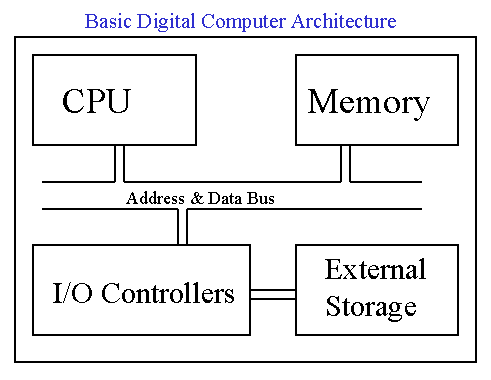
\includegraphics[width=0.85\textwidth]{figures/computer-architecture.png}
\end{figure}


Modern computer architecture --- the \textit{von Neumann} model --- has
evolved to systems that are fundamentally structured  as shown in Figure \ref{figure:computer_architecture},
where the processor and memory are tightly linked to one another, while
data storage is loosely coupled.  This architecture reflects that \emph{storage}
has been much slower than \emph{memory} since the introduction of core memory in
the 1950s.

This was not always the case: \emph{drum memory}, which predated core memory,
was both main memory and storage.  The introduction of core memory created
this bifurcation, as core memory was faster but more expensive.  Over time, core
memory was itself replaced with \acs{DRAM}~\cite{US3728695A}.  Storage technologies
moved from paper (punch cards and paper tape, for example) to magnetic media 
(tapes and disks).

Each of these divergent fields has undergone tremendous changes that did not remain
in lock step with one another: performance and density have increased for both
domains.  In recent years the two domains have begin to converge once again, with
storage moving to block-oriented non-volatile memories, such as flash 
memory.~\cite{bez2003introduction}

Memory technologies have continued to improve both in terms of performance --- \acs{DRAM}
was itself eclipsed by \acs{SRAM}~\cite{US4322675A} though though because \acs{SRAM} 
remains considerably more expensive than \acs{DRAM}, it is typically only used in performance
critical areas of modern computer systems (e.g., the central processing unit itself).

In \citeyear{moore1965cramming} Gordon Moore observed that the number of components that
could economically be added to an integrated circuit was increasing rapidly, an observation
that has come to be known as ``Moore's Law''.~\cite{moore1965cramming}  While most often quoted
in reference to processor technologies, the trend that Moore observed can also be observed
in memory technologies, particularly as density has led to increased memory capacities.

While magnetic storage technologies benefited from some aspects of the improvements in
integrated circuits, a fundamental characteristic of media was a significant delay in obtaining
the data --- the \textit{latency} inherent in the physical movement of the equipment imposed
a fundamental distinction that kept memory and storage separate in how they were handled by
software using the system.

\begin{figure}
    \centering
    \caption{Latency Numbers}\label{figure:jeff-dean-numbers}
    \emph{Source: Jonas B\'oner, https://gist.github.com/jboner/2841832}
    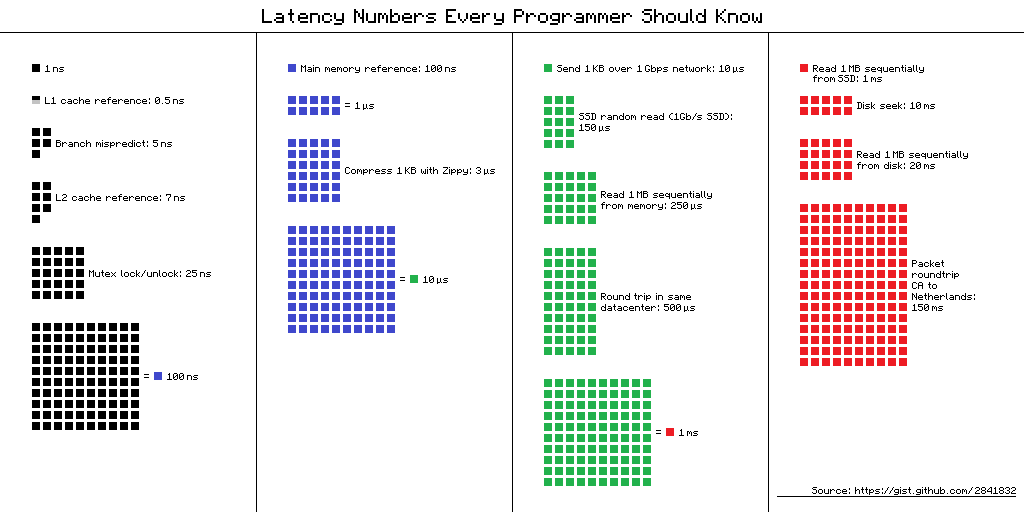
\includegraphics[width=0.85\textwidth]{figures/jeff-dean-numbers.png}
\end{figure}
    
Around ten years ago, Jeff Dean, a well-known distributed systems expert at Google gave a
presentation about the challenges of working with distributed systems.~\cite{jeff-dean:cs-295}
One of the slides in that presentation provided a succinct summary of the amount of time
to perform common operations within a computer system.  Figure \ref{figure:jeff-dean-numbers}
provides a graphic representation of the relative difference between these operations.~\cite{jboner:jeff-dean-numbers}
For the purposes of this work, the important point is to note that the speed of accessing
main memory at the time was approximately 100 nanoseconds. Reading 1MB of data from a disk
required \textbf{20 milliseconds}, half of which was the latency of the physical disk drive hardware.

\begin{figure}[b]
    \centering
    \caption{NVME Performance}\label{figure:nvme}
    \subcaptionbox[Bandwidth]{%
        Bandwidth%
        \label{figure:nvme:bandwidth}
    }
    [%
    0.45\textwidth
    ]%
    {%
        \includegraphics[width=0.45\textwidth]%
        {figures/sustained-throughput-100763047-large.jpg}%
    }%
    %\hspace{0.1\textwidth} % separation
    \subcaptionbox[Latency]{%
        Latency%
        \label{figure:nvme:latency}
    }
    [%
    0.45\textwidth
    ]%
    {%
        \includegraphics[width=0.45\textwidth]%
        {figures/seek-times-100763046-large.jpg}%
    }%
\end{figure}


Since that time, storage has undergone a tremendous shift due to the rapid development
and deployment of solid-state storage: \textit{persistent memory} that has been used to
construct devices which mimic the behavior of disk drives. In the span of roughly 10 years,
the bandwidth of non-volatile memory devices has increased dramatically, which led to the
introduction of higher-bandwidth interconnects between the storage device and the \acs{CPU}.
Currently, the highest speed interconnect \acs{NVMe} over \acs{PCIe} has a maximum theoretical
bandwidth of approximately 32GB/s.

Many of these changes have been driven by the increased density and decreased latency for
persistent memories. The convergence of this process increasingly appears to be a model
in which the boundary between \textit{memory} and \textit{storage} overlaps.  While
pragmatic engineering realities (ergo \textit{cost}) make it likely that slower but cheaper
storage options will continue to coexist with these new technologies, non-volatile memory
technologies will be utilized in performance critical areas to improve overall system performance.

Thus, in recent years we have seen \acs{DRAM}-like non-volatile memory solutions appear.  Frequently,
they have combined DRAM, non-volatile (flash) memory, and some backup power source ---
typically a large battery --- into providing large capacity, high performance, byte-addressable,
non-volatile memory, such as shown in Figure \ref{figure:scm}

\begin{figure}
    \centering
    \caption{Battery-Backed Hybrid DRAM/Flash Memory}\label{figure:scm}
    \emph{Source: RTC Magazine, http://archive.rtcmagazine.com/articles/view/102366}
    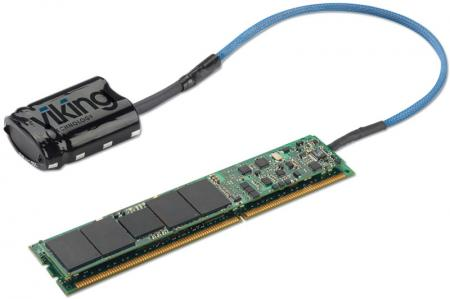
\includegraphics[width=0.65\textwidth]{figures/102366-2700_RTC11-PRTW-Viking-Fig1_medium.jpg}
\end{figure}

This type of ``storage class memory'' is not widely used, given its disadvantages, which include
cost, the need for external batteries, the lack of standardized support, and the relatively low
density offered --- often on par with \acs{DRAM}.

At the end of May, 2018 --- \textit{after} the commencement of working on this project, in fact,
Intel announced availability of their first \textit{byte-addressable} non-volatile memory modules,
with a form factor that makes them compatible with industry standard \acs{DDR4} 
memory.~\cite{anandtech:apache_pass}  While Intel has not confirmed the technology behind this
new memory, there has been considerable independent analysis indicating that the underlying
technology is \acs{PCM}.~\cite{malventano:2017:3DXPoint}

The ``hands-on'' analysis provided in this report is based upon Intel ``Apache Pass'' \acs{NVDIMM}
form-factor memory.  While interesting to have actual hardware to use in the evaluation, I have
tried to focus on insights that are not tied to the specific product.  This seems prudent because
Intel and Micron recently announced they would be terminating their joint development program 
next year.~\cite{Intel:3DXPoint:JDP:July:2018}

Commercialization of non-volatile memory technologies for the production of DIMM form factor
persistent memory devices is an active area.  These technologies include:

\begin{itemize}
    \item \acs{PCM} --- This is the basis of the Intel/Micron developed 3D XPoint memory and
    forms the basis of the Intel Apache Pass product (which will use the Optane\textsuperscript{tm} trade name
    when released.)
    \item \acs{MRAM} --- STT-MRAM is being used in high capacity enterprise SSD devices from IBM, and is
    available in a DIMM form factor, but does not yet appear to have achieved high densities though it
    does show high performance.~\cite{MRAM-info}
    \item \acs{FRAM} --- Ferroelectric Random Access Memory is commercially utilized non-volatile memory
    technology that has continues to be an area of active research in improving scalability.~\cite{mikolajick2018ferroelectric}
    \item \acs{ReRAM} --- Resistive Random Access Memory, the technology based upon the \textit{memristor}, continues
    to be yet another area of ongoing research.\cite{zhu2017resistive,lastras2018resistive}
    \item \acs{NRAM} --- Non-volatile Random Access Memory utilizes Carbon Nanotubes for data storage.  These memories
    are presently in production and in use in specialized environments due to the novel thermal characteristics of Carbon
    nanotubes.~\cite{gilmer2018nram}
\end{itemize}

Several of these are already used in specialized environment.  For the most promising, the challenge remains
commercializing the technology, often through scaling density or achieving economically viable cost/benefit levels.

In fact, it seems likely that several of these technologies will be used in the future for providing memory.  While
there is some value in evaluating the behavior of specific memory technology, it is somewhat ephemeral given the
ever-changing nature of the technology industry.

It is more useful to find insights, even from such focused study, that provide a general sense of understanding
about persistent memory.  To that end, I have considered a number of aspects of the behavior of non-volatile
memory:

\begin{itemize}
    \item \textbf{Failure Models} --- For any persistent data structure, it is imperative to understand the failure
    model of the domain. The challenge in this area is that storage experts are used to thinking of I/O related
    failure models, while processor behavior experts are used to considering consistency and correctness, but not
    persistence.

    \item \textbf{Performance} --- storage systems are traditionally high-latency.  There are write amplification
    issues that must be carefully evaluated.  Memory systems have concerns about cache behavior, the cost of
    consistency, and issues of memory locality because \acs{NUMA} architectures create unequal costs for accessing
    specific memory.

    \item \textbf{Consistency} --- persistence amplifies the cost of inconsistent state.  A traditional way to 
    recover from inconsistent machine state is to restart, which returns to a known-good state.  When memory
    is persistent, inconsistent states do not automatically resolve when the system restarts.

\end{itemize}

I discuss failure models in Chapter \ref{ch:Model} and insights gleaned from the
work with \acs{NVM} in Chapter \ref{ch:Discussion}.

\endinput

Any text after an \endinput is ignored.
You could put scraps here or things in progress.

% note that beyond this is the original content from the dissertation
% format.
%

This document provides a quick set of instructions for using the
\class{ubcdiss} class to write a dissertation in \LaTeX. 
Unfortunately this document cannot provide an introduction to using
\LaTeX.  The classic reference for learning \LaTeX\ is
\citeauthor{lamport-1994-ladps}'s
book~\cite{lamport-1994-ladps}.  There are also many freely-available
tutorials online;
\webref{http://www.andy-roberts.net/misc/latex/}{Andy Roberts' online
    \LaTeX\ tutorials}
seems to be excellent.
The source code for this docment, however, is intended to serve as
an example for creating a \LaTeX\ version of your dissertation.

We start by discussing organizational issues, such as splitting
your dissertation into multiple files, in
\autoref{sec:SuggestedThesisOrganization}.
We then cover the ease of managing cross-references in \LaTeX\ in
\autoref{sec:CrossReferences}.
We cover managing and using bibliographies with \BibTeX\ in
\autoref{sec:BibTeX}. 
We briefly describe typesetting attractive tables in
\autoref{sec:TypesettingTables}.
We briefly describe including external figures in
\autoref{sec:Graphics}, and using special characters and symbols
in \autoref{sec:SpecialSymbols}.
As it is often useful to track different versions of your dissertation,
we discuss revision control further in
\autoref{sec:DissertationRevisionControl}. 
We conclude with pointers to additional sources of information in
\autoref{sec:Conclusions}.

%%%%%%%%%%%%%%%%%%%%%%%%%%%%%%%%%%%%%%%%%%%%%%%%%%%%%%%%%%%%%%%%%%%%%%
\section{Suggested Thesis Organization}
\label{sec:SuggestedThesisOrganization}

The \acs{UBC} \acf{GPS} specifies a particular arrangement of the
components forming a thesis.\footnote{See
    \url{http://www.grad.ubc.ca/current-students/dissertation-thesis-preparation/order-components}}
This template reflects that arrangement.

In terms of writing your thesis, the recommended best practice for
organizing large documents in \LaTeX\ is to place each chapter in
a separate file.  These chapters are then included from the main
file through the use of \verb+\include{file}+.  A thesis might
be described as six files such as \file{intro.tex},
\file{relwork.tex}, \file{model.tex}, \file{eval.tex},
\file{discuss.tex}, and \file{concl.tex}.

We also encourage you to use macros for separating how something
will be typeset (\eg bold, or italics) from the meaning of that
something. 
For example, if you look at \file{intro.tex}, you will see repeated
uses of a macro \verb+\file{}+ to indicate file names.
The \verb+\file{}+ macro is defined in the file \file{macros.tex}.
The consistent use of \verb+\file{}+ throughout the text not only
indicates that the argument to the macro represents a file (providing
meaning or semantics), but also allows easily changing how
file names are typeset simply by changing the definition of the
\verb+\file{}+ macro.
\file{macros.tex} contains other useful macros for properly typesetting
things like the proper uses of the latinate \emph{exempli grati\={a}}
and \emph{id est} (\ie \verb+\eg+ and \verb+\ie+), 
web references with a footnoted \acs{URL} (\verb+\webref{url}{text}+),
as well as definitions specific to this documentation
(\verb+\latexpackage{}+).

%%%%%%%%%%%%%%%%%%%%%%%%%%%%%%%%%%%%%%%%%%%%%%%%%%%%%%%%%%%%%%%%%%%%%%
\section{Making Cross-References}
\label{sec:CrossReferences}

\LaTeX\ make managing cross-references easy, and the \latexpackage{hyperref}
package's\ \verb+\autoref{}+ command\footnote{%
    The \latexpackage{hyperref} package is included by default in this
    template.}
makes it easier still. 

A thing to be cross-referenced, such as a section, figure, or equation,
is \emph{labelled} using a unique, user-provided identifier, defined
using the \verb+\label{}+ command.  
The thing is referenced elsewhere using the \verb+\autoref{}+ command.
For example, this section was defined using:
\begin{lstlisting}
    \section{Making Cross-References}
    \label{sec:CrossReferences}
\end{lstlisting}
References to this section are made as follows:
\begin{lstlisting}
    We then cover the ease of managing cross-references in \LaTeX\
    in \autoref{sec:CrossReferences}.
\end{lstlisting}
\verb+\autoref{}+ takes care of determining the \emph{type} of the 
thing being referenced, so the example above is rendered as
\begin{quote}
    We then cover the ease of managing cross-references in \LaTeX\
    in \autoref{sec:CrossReferences}.
\end{quote}

The label is any simple sequence of characters, numbers, digits,
and some punctuation marks such as ``:'' and ``--''; there should
be no spaces.  Try to use a consistent key format: this simplifies
remembering how to make references.  This document uses a prefix
to indicate the type of the thing being referenced, such as \texttt{sec}
for sections, \texttt{fig} for figures, \texttt{tbl} for tables,
and \texttt{eqn} for equations.

For details on defining the text used to describe the type
of \emph{thing}, search \file{diss.tex} and the \latexpackage{hyperref}
documentation for \texttt{autorefname}.


%%%%%%%%%%%%%%%%%%%%%%%%%%%%%%%%%%%%%%%%%%%%%%%%%%%%%%%%%%%%%%%%%%%%%%
\section{Managing Bibliographies with \BibTeX}
\label{sec:BibTeX}

One of the primary benefits of using \LaTeX\ is its companion program,
\BibTeX, for managing bibliographies and citations.  Managing
bibliographies has three parts: (i) describing references,
(ii)~citing references, and (iii)~formatting cited references.

\subsection{Describing References}

\BibTeX\ defines a standard format for recording details about a
reference.  These references are recorded in a file with a
\file{.bib} extension.  \BibTeX\ supports a broad range of
references, such as books, articles, items in a conference proceedings,
chapters, technical reports, manuals, dissertations, and unpublished
manuscripts. 
A reference may include attributes such as the authors,
the title, the page numbers, the \ac{DOI}, or a \ac{URL}.  A reference
can also be augmented with personal attributes, such as a rating,
notes, or keywords.

Each reference must be described by a unique \emph{key}.\footnote{%
    Note that the citation keys are different from the reference
    identifiers as described in \autoref{sec:CrossReferences}.}
A key is a simple sequence of characters, numbers, digits, and some
punctuation marks such as ``:'' and ``--''; there should be no spaces. 
A consistent key format simiplifies remembering how to make references. 
For example:
\begin{quote}
   \fbox{\emph{last-name}}\texttt{-}\fbox{\emph{year}}\texttt{-}\fbox{\emph{contracted-title}}
\end{quote}
where \emph{last-name} represents the last name for the first author,
and \emph{contracted-title} is some meaningful contraction of the
title.  Then \citeauthor{kiczales-1997-aop}'s seminal article on
aspect-oriented programming~\cite{kiczales-1997-aop} (published in
\citeyear{kiczales-1997-aop}) might be given the key
\texttt{kiczales-1997-aop}.

An example of a \BibTeX\ \file{.bib} file is included as
\file{biblio.bib}.  A description of the format a \file{.bib}
file is beyond the scope of this document.  We instead encourage
you to use one of the several reference managers that support the
\BibTeX\ format such as
\webref{http://jabref.sourceforge.net}{JabRef} (multiple platforms) or
\webref{http://bibdesk.sourceforge.net}{BibDesk} (MacOS\,X only). 
These front ends are similar to reference manages such as
EndNote or RefWorks.


\subsection{Citing References}

Having described some references, we then need to cite them.  We
do this using a form of the \verb+\cite+ command.  For example:
\begin{lstlisting}
    \citet{kiczales-1997-aop} present examples of crosscutting 
    from programs written in several languages.
\end{lstlisting}
When processed, the \verb+\citet+ will cause the paper's authors
and a standardized reference to the paper to be inserted in the
document, and will also include a formatted citation for the paper
in the bibliography.  For example:
\begin{quote}
    \citet{kiczales-1997-aop} present examples of crosscutting 
    from programs written in several languages.
\end{quote}
There are several forms of the \verb+\cite+ command (provided
by the \latexpackage{natbib} package), as demonstrated in
\autoref{tbl:natbib:cite}.
Note that the form of the citation (numeric or author-year) depends
on the bibliography style (described in the next section).
The \verb+\citet+ variant is used when the author names form
an object in the sentence, whereas the \verb+\citep+ variant
is used for parenthetic references, more like an end-note.
Use \verb+\nocite+ to include a citation in the bibliography
but without an actual reference.
\nocite{rowling-1997-hpps}
\begin{table}
\caption{Available \texttt{cite} variants; the exact citation style
    depends on whether the bibliography style is numeric or author-year.}
\label{tbl:natbib:cite}
\centering
\begin{tabular}{lp{3.25in}}\toprule
Variant & Result \\
\midrule
% We cheat here to simulate the cite/citep/citet for APA-like styles
\verb+\cite+ & Parenthetical citation (\eg ``\cite{kiczales-1997-aop}''
    or ``(\citeauthor{kiczales-1997-aop} \citeyear{kiczales-1997-aop})'') \\
\verb+\citet+ & Textual citation: includes author (\eg
    ``\citet{kiczales-1997-aop}'' or
    or ``\citeauthor{kiczales-1997-aop} (\citeyear{kiczales-1997-aop})'') \\
\verb+\citet*+ & Textual citation with unabbreviated author list \\
\verb+\citealt+ & Like \verb+\citet+ but without parentheses \\
\verb+\citep+ & Parenthetical citation (\eg ``\cite{kiczales-1997-aop}''
    or ``(\citeauthor{kiczales-1997-aop} \citeyear{kiczales-1997-aop})'') \\
\verb+\citep*+ & Parenthetical citation with unabbreviated author list \\
\verb+\citealp+ & Like \verb+\citep+ but without parentheses \\
\verb+\citeauthor+ & Author only (\eg ``\citeauthor{kiczales-1997-aop}'') \\
\verb+\citeauthor*+ & Unabbreviated authors list 
    (\eg ``\citeauthor*{kiczales-1997-aop}'') \\
\verb+\citeyear+ & Year of citation (\eg ``\citeyear{kiczales-1997-aop}'') \\
\bottomrule
\end{tabular}
\end{table}

\subsection{Formatting Cited References}

\BibTeX\ separates the citing of a reference from how the cited
reference is formatted for a bibliography, specified with the
\verb+\bibliographystyle+ command. 
There are many varieties, such as \texttt{plainnat}, \texttt{abbrvnat},
\texttt{unsrtnat}, and \texttt{vancouver}.
This document was formatted with \texttt{abbrvnat}.
Look through your \TeX\ distribution for \file{.bst} files. 
Note that use of some \file{.bst} files do not emit all the information
necessary to properly use \verb+\citet{}+, \verb+\citep{}+,
\verb+\citeyear{}+, and \verb+\citeauthor{}+.

There are also packages available to place citations on a per-chapter
basis (\latexpackage{bibunits}), as footnotes (\latexpackage{footbib}),
and inline (\latexpackage{bibentry}).
Those who wish to exert maximum control over their bibliography
style should see the amazing \latexpackage{custom-bib} package.

%%%%%%%%%%%%%%%%%%%%%%%%%%%%%%%%%%%%%%%%%%%%%%%%%%%%%%%%%%%%%%%%%%%%%%
\section{Typesetting Tables}
\label{sec:TypesettingTables}

\citet{lamport-1994-ladps} made one grievous mistake
in \LaTeX: his suggested manner for typesetting tables produces
typographic abominations.  These suggestions have unfortunately
been replicated in most \LaTeX\ tutorials.  These
abominations are easily avoided simply by ignoring his examples
illustrating the use of horizontal and vertical rules (specifically
the use of \verb+\hline+ and \verb+|+) and using the
\latexpackage{booktabs} package instead.

The \latexpackage{booktabs} package helps produce tables in the form
used by most professionally-edited journals through the use of
three new types of dividing lines, or \emph{rules}.
% There are times that you don't want to use \autoref{}
Tables~\ref{tbl:natbib:cite} and~\ref{tbl:LaTeX:Symbols} are two
examples of tables typeset with the \latexpackage{booktabs} package.
The \latexpackage{booktabs} package provides three new commands
for producing rules:
\verb+\toprule+ for the rule to appear at the top of the table,
\verb+\midrule+ for the middle rule following the table header,
and \verb+\bottomrule+ for the bottom-most at the end of the table.
These rules differ by their weight (thickness) and the spacing before
and after.
A table is typeset in the following manner:
\begin{lstlisting}
    \begin{table}
    \caption{The caption for the table}
    \label{tbl:label}
    \centering
    \begin{tabular}{cc}
    \toprule
    Header & Elements \\
    \midrule
    Row 1 & Row 1 \\
    Row 2 & Row 2 \\
    % ... and on and on ...
    Row N & Row N \\
    \bottomrule
    \end{tabular}
    \end{table}
\end{lstlisting}
See the \latexpackage{booktabs} documentation for advice in dealing with
special cases, such as subheading rules, introducing extra space
for divisions, and interior rules.

%%%%%%%%%%%%%%%%%%%%%%%%%%%%%%%%%%%%%%%%%%%%%%%%%%%%%%%%%%%%%%%%%%%%%%
\section{Figures, Graphics, and Special Characters}
\label{sec:Graphics}

Most \LaTeX\ beginners find figures to be one of the more challenging
topics.  In \LaTeX, a figure is a \emph{floating element}, to be
placed where it best fits.
The user is not expected to concern him/herself with the placement
of the figure.  The figure should instead be labelled, and where
the figure is used, the text should use \verb+\autoref+ to reference
the figure's label.
\autoref{fig:latex-affirmation} is an example of a figure.
\begin{figure}
    \centering
    % For the sake of this example, we'll just use text
    %\includegraphics[width=3in]{file}
    \Huge{\textsf{\LaTeX\ Rocks!}}
    \caption{Proof of \LaTeX's amazing abilities}
    \label{fig:latex-affirmation}   % label should change
\end{figure}
A figure is generally included as follows:
\begin{lstlisting}
    \begin{figure}
    \centering
    \includegraphics[width=3in]{file}
    \caption{A useful caption}
    \label{fig:fig-label}   % label should change
    \end{figure}
\end{lstlisting}
There are three items of note:
\begin{enumerate}
\item External files are included using the \verb+\includegraphics+
    command.  This command is defined by the \latexpackage{graphicx} package
    and can often natively import graphics from a variety of formats.
    The set of formats supported depends on your \TeX\ command processor.
    Both \texttt{pdflatex} and \texttt{xelatex}, for example, can
    import \textsc{gif}, \textsc{jpg}, and \textsc{pdf}.  The plain
    version of \texttt{latex} only supports \textsc{eps} files.

\item The \verb+\caption+ provides a caption to the figure. 
    This caption is normally listed in the List of Figures; you
    can provide an alternative caption for the LoF by providing
    an optional argument to the \verb+\caption+ like so:
    \begin{lstlisting}
    \caption[nice shortened caption for LoF]{%
	longer detailed caption used for the figure}
    \end{lstlisting}
    \ac{GPS} generally prefers shortened single-line captions
    in the LoF: multiple-line captions are a bit unwieldy.

\item The \verb+\label+ command provides for associating a unique, user-defined,
    and descriptive identifier to the figure.  The figure can be
    can be referenced elsewhere in the text with this identifier
    as described in \autoref{sec:CrossReferences}.
\end{enumerate}
See Keith Reckdahl’s excellent guide for more details,
\webref{http://www.ctan.org/tex-archive/info/epslatex.pdf}{\emph{Using
imported graphics in LaTeX2e}}.

\section{Special Characters and Symbols}
\label{sec:SpecialSymbols}

\LaTeX\ appropriates many common symbols for its own purposes,
with some used for commands (\ie \verb+\{}&%+) and
mathematics (\ie \verb+$^_+), and others are automagically transformed
into typographically-preferred forms (\ie \verb+-`'+) or to
completely different forms (\ie \verb+<>+).
\autoref{tbl:LaTeX:Symbols} presents a list of common symbols and
their corresponding \LaTeX\ commands.  A much more comprehensive list 
of symbols and accented characters is available at:
\url{http://www.ctan.org/tex-archive/info/symbols/comprehensive/}
\begin{table}
\caption{Useful \LaTeX\ symbols}\label{tbl:LaTeX:Symbols}
\centering\begin{tabular}{ccp{0.5cm}cc}\toprule
\LaTeX & Result && \LaTeX & Result \\
\midrule
    \verb+\texttrademark+ & \texttrademark && \verb+\&+ & \& \\
    \verb+\textcopyright+ & \textcopyright && \verb+\{ \}+ & \{ \} \\
    \verb+\textregistered+ & \textregistered && \verb+\%+ & \% \\
    \verb+\textsection+ & \textsection && \verb+\verb!~!+ & \verb!~! \\
    \verb+\textdagger+ & \textdagger && \verb+\$+ & \$ \\
    \verb+\textdaggerdbl+ & \textdaggerdbl && \verb+\^{}+ & \^{} \\
    \verb+\textless+ & \textless && \verb+\_+ & \_ \\
    \verb+\textgreater+ & \textgreater && \\
\bottomrule
\end{tabular}
\end{table}

%%%%%%%%%%%%%%%%%%%%%%%%%%%%%%%%%%%%%%%%%%%%%%%%%%%%%%%%%%%%%%%%%%%%%%
\section{Changing Page Widths and Heights}

The \class{ubcdiss} class is based on the standard \LaTeX\ \class{book}
class~\cite{lamport-1994-ladps} that selects a line-width to carry
approximately 66~characters per line.  This character density is
claimed to have a pleasing appearance and also supports more rapid
reading~\cite{bringhurst-2002-teots}.  I would recommend that you
not change the line-widths!

\subsection{The \texttt{geometry} Package}

Some students are unfortunately saddled with misguided supervisors
or committee members whom believe that documents should have the
narrowest margins possible.  The \latexpackage{geometry} package is
helpful in such cases.  Using this package is as simple as:
\begin{lstlisting}
    \usepackage[margin=1.25in,top=1.25in,bottom=1.25in]{geometry}
\end{lstlisting}
You should check the package's documentation for more complex uses.

\subsection{Changing Page Layout Values By Hand}

There are some miserable students with requirements for page layouts
that vary throughout the document.  Unfortunately the
\latexpackage{geometry} can only be specified once, in the document's
preamble.  Such miserable students must set \LaTeX's layout parameters
by hand:
\begin{lstlisting}
    \setlength{\topmargin}{-.75in}
    \setlength{\headsep}{0.25in}
    \setlength{\headheight}{15pt}
    \setlength{\textheight}{9in}
    \setlength{\footskip}{0.25in}
    \setlength{\footheight}{15pt}

    % The *sidemargin values are relative to 1in; so the following
    % results in a 0.75 inch margin
    \setlength{\oddsidemargin}{-0.25in}
    \setlength{\evensidemargin}{-0.25in}
    \setlength{\textwidth}{7in}       % 1.1in margins (8.5-2*0.75)
\end{lstlisting}
These settings necessarily require assuming a particular page height
and width; in the above, the setting for \verb+\textwidth+ assumes
a \textsc{US} Letter with an 8.5'' width.
The \latexpackage{geometry} package simply uses the page height and
other specified values to derive the other layout values.
The
\href{http://tug.ctan.org/tex-archive/macros/latex/required/tools/layout.pdf}{\texttt{layout}}
package provides a
handy \verb+\layout+ command to show the current page layout
parameters. 


\subsection{Making Temporary Changes to Page Layout}

There are occasions where it becomes necessary to make temporary
changes to the page width, such as to accomodate a larger formula. 
The \latexmiscpackage{chngpage} package provides an \env{adjustwidth}
environment that does just this.  For example:
\begin{lstlisting}
    % Expand left and right margins by 0.75in
    \begin{adjustwidth}{-0.75in}{-0.75in}
    % Must adjust the perceived column width for LaTeX to get with it.
    \addtolength{\columnwidth}{1.5in}
    \[ an extra long math formula \]
    \end{adjustwidth}
\end{lstlisting}


%%%%%%%%%%%%%%%%%%%%%%%%%%%%%%%%%%%%%%%%%%%%%%%%%%%%%%%%%%%%%%%%%%%%%%
\section{Keeping Track of Versions with Revision Control}
\label{sec:DissertationRevisionControl}

Software engineers have used \acf{RCS} to track changes to their
software systems for decades.  These systems record the changes to
the source code along with context as to why the change was required.
These systems also support examining and reverting to particular
revisions from their system's past.

An \ac{RCS} can be used to keep track of changes to things other
than source code, such as your dissertation.  For example, it can
be useful to know exactly which revision of your dissertation was
sent to a particular committee member.  Or to recover an accidentally
deleted file, or a badly modified image.  With a revision control
system, you can tag or annotate the revision of your dissertation
that was sent to your committee, or when you incorporated changes
from your supervisor.

Unfortunately current revision control packages are not yet targetted
to non-developers.  But the Subversion project's
\webref{http://tortoisesvn.net/docs/release/TortoiseSVN_en/}{TortoiseSVN}
has greatly simplified using the Subversion revision control system
for Windows users.  You should consult your local geek.

A simpler alternative strategy is to create a GoogleMail account
and periodically mail yourself zipped copies of your dissertation.

%%%%%%%%%%%%%%%%%%%%%%%%%%%%%%%%%%%%%%%%%%%%%%%%%%%%%%%%%%%%%%%%%%%%%%
\section{Recommended Packages}

The real strength to \LaTeX\ is found in the myriad of free add-on
packages available for handling special formatting requirements.
In this section we list some helpful packages.

\subsection{Typesetting}

\begin{description}
\item[\latexpackage{enumitem}:]
    Supports pausing and resuming enumerate environments.

\item[\latexpackage{ulem}:]
    Provides two new commands for striking out and crossing out text
    (\verb+\sout{text}+ and \verb+\xout{text}+ respectively)
    The package should likely
    be used as follows:
    \begin{verbatim}
    \usepackage[normalem,normalbf]{ulem}
    \end{verbatim}
    to prevent the package from redefining the emphasis and bold fonts.

\item[\latexpackage{chngpage}:]
    Support changing the page widths on demand.

\item[\latexpackage{mhchem}:] 
    Support for typesetting chemical formulae and reaction equations.

\end{description}

Although not a package, the
\webref{http://www.ctan.org/tex-archive/support/latexdiff/}{\texttt{latexdiff}}
command is very useful for creating changebar'd versions of your
dissertation.


\subsection{Figures, Tables, and Document Extracts}

\begin{description}
\item[\latexpackage{pdfpages}:]
    Insert pages from other PDF files.  Allows referencing the extracted
    pages in the list of figures, adding labels to reference the page
    from elsewhere, and add borders to the pages.

\item[\latexpackage{subfig}:]
    Provides for including subfigures within a figure, and includes
    being able to separately reference the subfigures.  This is a
    replacement for the older \texttt{subfigure} environment.

\item[\latexpackage{rotating}:]
    Provides two environments, sidewaystable and sidewaysfigure,
    for typesetting tables and figures in landscape mode.  

\item[\latexpackage{longtable}:]
    Support for long tables that span multiple pages.

\item[\latexpackage{tabularx}:]
    Provides an enhanced tabular environment with auto-sizing columns.

\item[\latexpackage{ragged2e}:]
    Provides several new commands for setting ragged text (\eg forms
    of centered or flushed text) that can be used in tabular
    environments and that support hyphenation.

\end{description}


\subsection{Bibliography Related Packages}

\begin{description}
\item[\latexpackage{bibunits}:]
    Support having per-chapter bibliographies.

\item[\latexpackage{footbib}:]
    Cause cited works to be rendered using footnotes.

\item[\latexpackage{bibentry}:] 
    Support placing the details of a cited work in-line.

\item[\latexpackage{custom-bib}:]
    Generate a custom style for your bibliography.

\end{description}


%%%%%%%%%%%%%%%%%%%%%%%%%%%%%%%%%%%%%%%%%%%%%%%%%%%%%%%%%%%%%%%%%%%%%%
\section{Moving On}
\label{sec:Conclusions}

At this point, you should be ready to go.  Other handy web resources:
\begin{itemize}
\item \webref{http://www.ctan.org}{\ac{CTAN}} is \emph{the} comprehensive
    archive site for all things related to \TeX\ and \LaTeX. 
    Should you have some particular requirement, somebody else is
    almost certainly to have had the same requirement before you,
    and the solution will be found on \ac{CTAN}.  The links to
    various packages in this document are all to \ac{CTAN}.

\item An online
    \webref{http://www.ctan.org/get/info/latex2e-help-texinfo/latex2e.html}{%
	reference to \LaTeX\ commands} provides a handy quick-reference
    to the standard \LaTeX\ commands.

\item The list of 
    \webref{http://www.tex.ac.uk/cgi-bin/texfaq2html?label=interruptlist}{%
	Frequently Asked Questions about \TeX\ and \LaTeX}
    can save you a huge amount of time in finding solutions to
    common problems.

\item The \webref{http://www.tug.org/tetex/tetex-texmfdist/doc/}{te\TeX\
    documentation guide} features a very handy list of the most useful
    packages for \LaTeX\ as found in \ac{CTAN}.

\item The
\webref{http://www.ctan.org/tex-archive/macros/latex/required/graphics/grfguide.pdf}{\texttt{color}}
    package, part of the graphics bundle, provides handy commands
    for changing text and background colours.  Simply changing
    text to various levels of grey can have a very 
    \textcolor{greytext}{dramatic effect}.


\item If you're really keen, you might want to join the
    \webref{http://www.tug.org}{\TeX\ Users Group}.

\end{itemize}





%    2. Main body
% Generally recommended to put each chapter into a separate file
%% The following is a directive for TeXShop to indicate the main file
%%!TEX root = report.tex

\chapter{Related Work}
\label{ch:RelatedWork}

The field of non-volatile memory is one with a long history.  As noted in Chapter \ref{ch:Introduction}, 
early memories were, in fact, persistent and this led to models in which memory and storage were viewed
as equivalent storage mechanisms.~\cite{corbato1965introduction}  The introduction of dynamic ram (\acs{DRAM})
led to the bifurcation in storage technologies between high-speed but ephemeral (``memory'') and low-speed
but persistent (``media'').~\cite{US3728695A}

Our modern model of storage has evolved as well, from the punch cards of the late 19th century~\cite{truesdell1965development},
to more modern media based magnetic devices, such as tape (ca. 1935) and other forms of magnetic
media.~\cite{feynman1992there, hoagland2003history}

The introduction of flash memory~\cite{masuoka1984new} led to flash storage devices.  Progress in this area has led to the
emergence of solid state disk drives.~\cite{clay1995flash}  \acs{SSD}s today are often the primary storage device of numerous
computers, despite their higher cost than traditional hard disks, due to their performance characteristics.

The push to make \acs{SSD}s faster has led to a rapid progression of bus technologies that permit exploitation of the 
increasing bandwidth and decreasing latency of such devices.  The (re)-convergence of storage and memory has been demonstrated 
and discussed for more than 20 years.\cite{wu1994envy,mogul2009operating,Nalli:2017:APM:3093336.3037730,Nalli:2017:APM:3093337.3037730,
Nalli:2017:APM:3037697.3037730,kolli2017architecting,joshi2015efficient}  
The advent of \acs{PCM} was one of those promising
technologies.~\cite{chen2016review}  The research community has explored this area extensively in the ensuing years in such topics as:

\begin{itemize}

    \item Memory Management:\cite{volos2011mnemosyne,Oukid:2017:MMT:3137628.3137629,yu2017redesign}
    \item Data Structures:\cite{Friedman:2018:PLQ:3178487.3178490,Memaripour:2017:AIU:3064176.3064215,lee2017wort,sha2018towards,zhang2018simpo,
kim2018clfb,wang2018persisting,nawab2017dali,lee2018write,oukid2017data,venkataraman2011consistent,chen2015persistent,222591,
zuo2017write,zuo2018write}
    \item Multi-threading: \cite{Hsu:2017:NPP:3064176.3064204}
    \item Programming: \cite{Kolli:2017:LP:3079856.3080229,Kolli:2017:LP:3140659.3080229,marathe2017persistent}
    \item File Systems:\cite{kannan2018designing,liu2018hmfs}
    \item Logging:\cite{Cohen:2017:ELN:3152284.3133891,shin2017proteus}
    \item Crash Consistency:\cite{Pillai:2017:ACC:3141876.3119897,wei2017transactional}
    \item Address Translation:\cite{Chen:2017:ESP:3123939.3124543,liu2017durable,wang2017hardware}
    \item Database:\cite{arulraj2017build,Oukid:2014:SHS:2619228.2619236,arulraj2015let}
    \item Checkpointing: \cite{zhang2017fine,giles2017continuous}
    \item Key-Value Stores:\cite{huang2018nvht,chen2017udorn,kim2017papyruskv,liu2017librekv,zhou2016nvht,wu2016nvmcached}
    \item Transations:\cite{marathe2018persistent}
\end{itemize}

Prior work has been done with a variety of models for simulating the behavior of \acs{NVM}.  Indeed, my
initial investigation was to determine the viability of investigating some of the considerations described
in Chapter \ref{ch:Introduction} via simulation.  Ultimately, I was able to gain access to an Intel Apache
Pass research system for performing this research.

Thus, one key difference between the prior work and the work described in this report is the use of actual
hardware.  As expected, that hardware does not behave as predicted.  I will discuss this further in Chapters \ref{ch:Results}
\& \ref{ch:Discussion}. 

\endinput


%% The following is a directive for TeXShop to indicate the main file
%%!TEX root = report.tex

\chapter{Model}
\label{ch:Model}

\section{Failure Models}\label{section:model:failure}


\section{Methodology}

%% The following is a directive for TeXShop to indicate the main file
%%!TEX root = report.tex

\chapter{Results}
\label{ch:Results}

\section{Test Hardware}

The primary system for testing was provided by Intel Research; this was physical hardware
and I had console level access to the system --- in fact, I reinstalled Fedora on the
system at one point.  My own test runs collected data on the system configuration.  I
capture that information here.

The Linux version (notably the kernel) was a current version at the time of testing:

\begin{verbatim}
# uname -a
  Linux intelsdp1044 4.17.12-200.fc28.x86_64 #1 \
  SMP Fri Aug 3 15:01:13 UTC 2018 x86_64 x86_64 \
  x86_64 GNU/Linux
\end{verbatim}

It included support for NVM as part of the base release package --- this was \textit{not}
a custom build.

The CPU information for the system is described in Tables \ref{table:results:hardware} \& \ref{table:results:hardware:2}.

\begin{table}
    \caption{Hardware Configuration Information (\textbf{lscpu}) Part 1}\label{table:results:hardware}
    \begin{tabular}{@{}cl@{}}
        Characteristic & Value  \\ \toprule
        Architecture &  x86\_64 \\
        CPU op-mode(s)&      32-bit, 64-bit \\
        Byte Order&          Little Endian \\
        CPU(s)&              96 \\
        On-line CPU(s) list& 0-95 \\
        Thread(s) per core&  2 \\
        Core(s) per socket&  24 \\
        Socket(s)&           2 \\
        NUMA node(s)&        2 \\
        Vendor ID&           GenuineIntel \\
        CPU family&          6 \\ 
        Model&               85 \\ 
        Model name&          Genuine Intel(R) CPU 0000\%@ \\
        Stepping&            5 \\
        CPU MHz&             2899.999 \\
        CPU max MHz&         3700.0000 \\
        CPU min MHz&         1000.0000 \\
        BogoMIPS&            4400.00 \\
        Virtualization&      VT-x \\
        L1d cache&           32K \\
        L1i cache&           32K \\
        L2 cache&            1024K \\
        L3 cache&            33792K \\
        NUMA node0 CPU(s)&   0-23,48-71 \\
        NUMA node1 CPU(s)&   24-47,72-95 \\
        \bottomrule
    \end{tabular}%
\end{table}

\begin{table}
        \caption{Hardware Configuration Information (\textbf{lscpu}) Part 2}\label{table:results:hardware:2}
        \begin{tabular}{@{}cl@{}}
        Flags & fpu vme de pse tsc msr pae mce cx8 apic sep \\
        & mtrr pge mca cmov pat pse36 clflush dts acpi \\
        & mmx fxsr sse sse2 ss ht tm pbe syscall nx pdpe1gb \\
        & rdtscp lm constant\_tsc art arch\_perfmon pebs \\
        & bts rep\_good nopl xtopology nonstop\_tsc cpuid \\
        & aperfmperf pni pclmulqdq dtes64 monitor ds\_cpl vmx \\
        & smx est tm2 ssse3 sdbg fma cx16 xtpr pdcm pcid dca \\
        & sse4\_1 sse4\_2 x2apic movbe popcnt aes xsave avx \\
        & f16c rdrand lahf\_lm abm 3dnowprefetch cpuid\_fault \\
        & epb cat\_l3 cdp\_l3 invpcid\_single pti intel\_ppin \\
        & mba ibrs ibpb stibp tpr\_shadow vnmi flexpriority \\
        & ept vpid fsgsbase tsc\_adjust bmi1 hle avx2 smep \\
        & bmi2 erms invpcid rtm cqm mpx rdt\_a avx512f \\ 
        & avx512dq rdseed adx smap clflushopt clwb intel\_pt \\
        & avx512cd avx512bw avx512vl xsaveopt xsavec xgetbv1 \\
        & xsaves cqm\_llc cqm\_occup\_llc cqm\_mbm\_total \\
        & cqm\_mbm\_local dtherm ida arat pln pts hwp \\
        & hwp\_act\_window hwp\_epp hwp\_pkg\_req pku ospke \\
        \bottomrule
    \end{tabular}%
\end{table}

Memory in the system consisted of 12 32GB DRAM modules and 12 249GB NVM modules.  This information
was displayed using the \verb+dmidecode --type 17+ to display information specific to the memory
modules installed on the machine.

DRAM modules appeared like:

\begin{verbatim}
    Handle 0x0026, DMI type 17, 40 bytes
Memory Device
	Array Handle: 0x0024
	Error Information Handle: Not Provided
	Total Width: 72 bits
	Data Width: 64 bits
	Size: 32 GB
	Form Factor: DIMM
	Set: None
	Locator: CPU1_DIMM_A1
	Bank Locator: NODE 1
	Type: DDR4
	Type Detail: Synchronous
	Speed: 2666 MT/s
	Manufacturer: Micron
	Serial Number: 18B132B8
	Asset Tag:  
	Part Number: 36ASF4G72PZ-2G6H1   
	Rank: 2
	Configured Clock Speed: 2666 MT/s
	Minimum Voltage: 1.2 V
	Maximum Voltage: 1.2 V
	Configured Voltage: 1.2 V
\end{verbatim}

NVM modules appeared like:

\begin{verbatim}
    Handle 0x0028, DMI type 17, 40 bytes
Memory Device
	Array Handle: 0x0024
	Error Information Handle: Not Provided
	Total Width: 72 bits
	Data Width: 64 bits
	Size: 255680 MB
	Form Factor: DIMM
	Set: None
	Locator: CPU1_DIMM_A2
	Bank Locator: NODE 1
	Type: DDR4
	Type Detail: Synchronous Non-Volatile
	Speed: 2666 MT/s
	Manufacturer: Intel
	Serial Number: 00000310
	Asset Tag:  
	Part Number: 8089A2173800000310  
	Rank: 1
	Configured Clock Speed: 2666 MT/s
	Minimum Voltage: 1.2 V
	Maximum Voltage: 1.2 V
	Configured Voltage: 1.2 V
\end{verbatim}

I have omitted all but the first instance of each for the sake of brevity; full logs are
available.

Similarly, using the \verb+lshw+ command in Linux, I captured detailed information about 
the system.  The following is the summary information about all memory installed in the
system:

\begin{verbatim}
    *-memory
    description: System Memory
    physical id: 24
    slot: System board or motherboard
    size: 3380GiB
    capabilities: ecc
    configuration: errordetection=ecc
\end{verbatim}

Similarly, this is the information about the first DIMM module:

\begin{verbatim}
  *-bank:0
       description: DIMM DDR4 Synchronous 2666 MHz (0.4 ns)
       product: 36ASF4G72PZ-2G6H1
       vendor: Micron
       physical id: 0
       serial: 18B132B8
       slot: CPU1_DIMM_A1
       size: 32GiB
       width: 64 bits
       clock: 2666MHz (0.4ns)
\end{verbatim}

Note that this provides different, but consistent information.  For example, the
serial numbers match between the two commands.

The NVM information:

\begin{verbatim}
  *-bank:1
       description: DIMM DDR4 Synchronous Non-volatile 2666 MHz (0.4 ns)
       product: 8089A2173800000310
       vendor: Intel
       physical id: 1
       serial: 00000310
       slot: CPU1_DIMM_A2
       size: 249GiB
       width: 64 bits
       clock: 2666MHz (0.4ns)
\end{verbatim}

Again, further information has been omitted but is available.

Only three of the NVM modules were provisioned: two for node 0, one for node 1.  These were
\acs{DAX} enabled, with xfs formatted for two of them, and ext4 for one of them.

\begin{verbatim}
# mount
/dev/pmem0 on /mnt/pmem0p1 type xfs (rw,relatime,seclabel,attr2,dax,inode64,noquota)
/dev/pmem2 on /mnt/pmem2 type ext4 (rw,relatime,seclabel,dax)
/dev/pmem10 on /mnt/pmem10 type xfs (rw,relatime,seclabel,attr2,dax,inode64,noquota)
\end{verbatim}

\textit{Note: I have omitted the non-\acs{DAX} volumes here.}  All three were mounted in \acs{DAX}
mode, ensuring that memory mapped files within those file systems were directly accessed by the
test application.

The \verb+ndctl+ command was used to capture information about the NVM provisioning as well:

\begin{verbatim}
    ndctl list --namespaces  --human
    [
      {
        "dev":"namespace0.0",
        "mode":"fsdax",
        "map":"dev",
        "size":"245.11 GiB (263.18 GB)",
        "uuid":"f05281b4-dfa7-4f48-ab8b-41d1f54205aa",
        "raw_uuid":"c6c12d35-853d-418a-8602-846d3fd6091c",
        "sector_size":512,
        "blockdev":"pmem0",
        "numa_node":0
      },
      {
        "dev":"namespace2.0",
        "mode":"fsdax",
        "map":"dev",
        "size":"245.11 GiB (263.18 GB)",
        "uuid":"44071681-9ffa-4df4-bd51-7c51092a83e4",
        "raw_uuid":"ee045c93-52e0-4d5e-9670-7bc82ce691d6",
        "sector_size":512,
        "blockdev":"pmem2",
        "numa_node":0
      },
      {
        "dev":"namespace10.0",
        "mode":"fsdax",
        "map":"dev",
        "size":"245.11 GiB (263.18 GB)",
        "uuid":"a755e8a2-c6ad-426f-8841-cf393bc2b4f9",
        "raw_uuid":"2f6e6311-7a52-4fc3-ac97-763454d18370",
        "sector_size":512,
        "blockdev":"pmem10",
        "numa_node":1
      }
    ]
\end{verbatim}

None of the NVM modules are striped (a potential configuration done via a software striping driver in Linux)
and the sizes correspond to NVM in a single DIMM location.

Finally, I used the \verb+ipmctl+ utility, which is available as part of the various Linux releases (including
Fedora 28, which I used).  It is the \textit{Intel persistent memory control} application.

\begin{verbatim}
# ipmctl show -topology
DimmID	MemoryType	Capacity	PhysicalID	DeviceLocator
0x0001	DCPMEM		249.6 GiB	0x0028		CPU1_DIMM_A2
0x0011	DCPMEM		249.6 GiB	0x002c		CPU1_DIMM_B2
0x0021	DCPMEM		249.6 GiB	0x0030		CPU1_DIMM_C2
0x0101	DCPMEM		249.6 GiB	0x0036		CPU1_DIMM_D2
0x0111	DCPMEM		249.6 GiB	0x003a		CPU1_DIMM_E2
0x0121	DCPMEM		249.6 GiB	0x003e		CPU1_DIMM_F2
0x1011	DCPMEM		249.6 GiB	0x0048		CPU2_DIMM_B2
0x1021	DCPMEM		249.6 GiB	0x004c		CPU2_DIMM_C2
0x1001	DCPMEM		249.6 GiB	0x0044		CPU2_DIMM_A2
0x1111	DCPMEM		249.6 GiB	0x0056		CPU2_DIMM_E2
0x1121	DCPMEM		249.6 GiB	0x005a		CPU2_DIMM_F2
0x1101	DCPMEM		249.6 GiB	0x0052		CPU2_DIMM_D2
N/A	DDR4		32.0 GiB	0x0026		CPU1_DIMM_A1
N/A	DDR4		32.0 GiB	0x002a		CPU1_DIMM_B1
N/A	DDR4		32.0 GiB	0x002e		CPU1_DIMM_C1
N/A	DDR4		32.0 GiB	0x0034		CPU1_DIMM_D1
N/A	DDR4		32.0 GiB	0x0038		CPU1_DIMM_E1
N/A	DDR4		32.0 GiB	0x003c		CPU1_DIMM_F1
N/A	DDR4		32.0 GiB	0x0042		CPU2_DIMM_A1
N/A	DDR4		32.0 GiB	0x0046		CPU2_DIMM_B1
N/A	DDR4		32.0 GiB	0x004a		CPU2_DIMM_C1
N/A	DDR4		32.0 GiB	0x0050		CPU2_DIMM_D1
N/A	DDR4		32.0 GiB	0x0054		CPU2_DIMM_E1
N/A	DDR4		32.0 GiB	0x0058		CPU2_DIMM_F1
\end{verbatim}

This captures the system configuration in a compact form, demonstrating the full amount of memory on
the test system.


\section{Intel Memory Latency Checker}\label{section:results:mlc}

The measurements in this section were collected using the Intel Memory Latency Checker, a tool
developed by Intel to evaluate memory bandwidth and latency.  Version 3.5 includes explicit
support for evaluating DRAM and NVM.  It is NUMA aware and can be used for evaluating both
node-local as well as node-remote memories.~\cite{IntelMLC35}

I note that the provided documentation for this tool does not describe some modes of
this tool that are, in fact, used in this evaluation.  Further, actually enabling the
correct testing mode for NVM is not easy to reproduce from the information available.
Thus, when reporting specific results I have included the command line switches used
as part of the testing. 

The tests considered in this section all used a zero injection latency (\texttt{-d0},)
as this represents the highest workload against the given memory --- latency injection
provides a simple mechanism for evaluating performance on workloads that are not
pushing the bandwidth boundary.  While I did perform evaluations with higher
injection rates, I have chosen to omit that additional data from this report.

Each specific test run uses various flags to control the behavior.  Unless
otherwise noted, all tests used the \verb+--loaded_latency+ option, which
means that the test utility is measuring the latency of the memory with
some load imposed.

Note that for all tests, \textbf{core 0} is used for measurements.  Thus, when
we report 3 cores in use, two of them are generating load and one is performing
the latency measurements.

For the various tests I use the switches as shown in Table \ref{mlc:switches}.

\begin{table}
    \caption{MLC switches used during testing}\label{mlc:switches}
    \begin{tabular}{@{}clc@{}}
        Switch & Effect & See Section \\ \toprule
        \verb+-d+ & Latency injection (seconds) &  \\
        \verb+-t+ & Test time (seconds) &  \\
        \verb+-l+ & Stride size (bytes) & \\
        \verb+-R+ & Read-only workload & \ref{baseline:dram}, \ref{baseline:nvm} \\
        \verb+-W2+ & Read-Write 2:1 Workload & \ref{chart:sequential:W2} \ref{chart:random:W2} \\ 
        \verb+-W3+ & Read-Write 3:1 Workload & \ref{chart:sequential:w3} \\
        \verb+-W5+ & Read-Write 1:1 Workload & \ref{chart:random:W5} \ref{chart:sequential:W5} \\
        \verb+-W6+ & Non-Temporal Write Workload & \ref{chart:random:w6} \ref{chart:sequential:W6} \\
        \verb+-W7+ & Read-Non-Temporal-Write 2:1 Workload & \ref{chart:random:W7} \ref{chart:sequential:W7} \\
        \verb+-W8+ & Read-Non-Temporal-Write 1:1 Workload  & \ref{chart:random:W8} \\
        \verb+-W10+ & Read-Non-Temporal-Write 3:1 (Streaming Triad) & \ref{chart:sequential:W10} \\ \bottomrule
    \end{tabular}%
\end{table}

Note that reported stride sizes were 16, 32, 64, 128, 256, 512, 1024, and 2048 in all cases.
In a few cases I report 4096, but for many tests that stride size failed to work properly
with the given test.  Similarly, I tested sizes below 16 bytes but found that it frequently
failed.

\subsection{Sanity Check}

\begin{figure}
    \centering
    \caption{Bandwidth Evaluation of Test System against Intel Reference}\label{chart:aep:bw}
    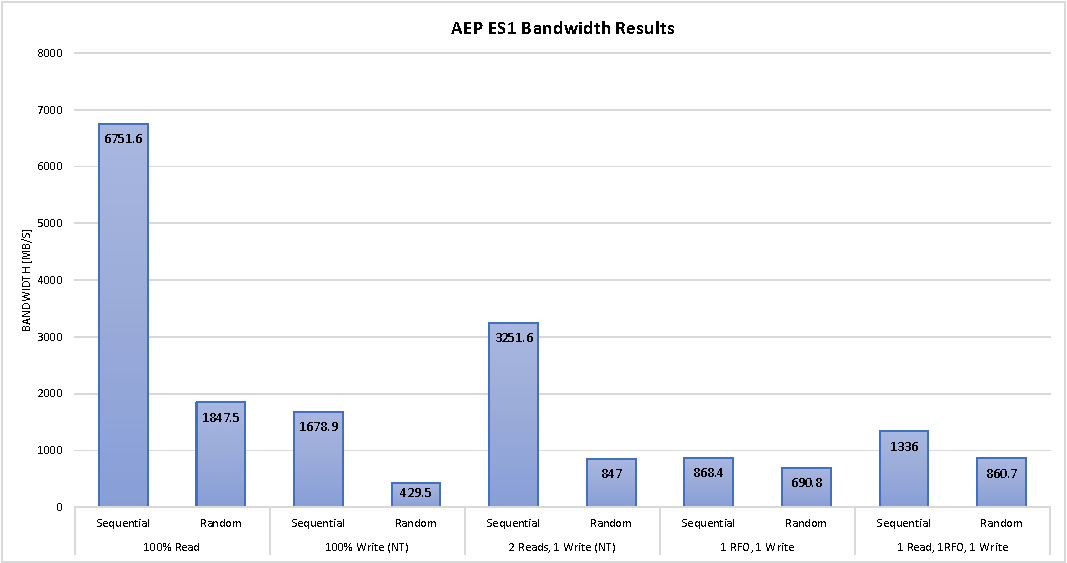
\includegraphics[scale=0.5]{charts/aep_eval_bandwidth-crop.pdf}
\end{figure}

\begin{figure}
    \centering
    \caption{Idle Latency Evaluation of Test System against Intel Reference}\label{chart:aep:idle}
    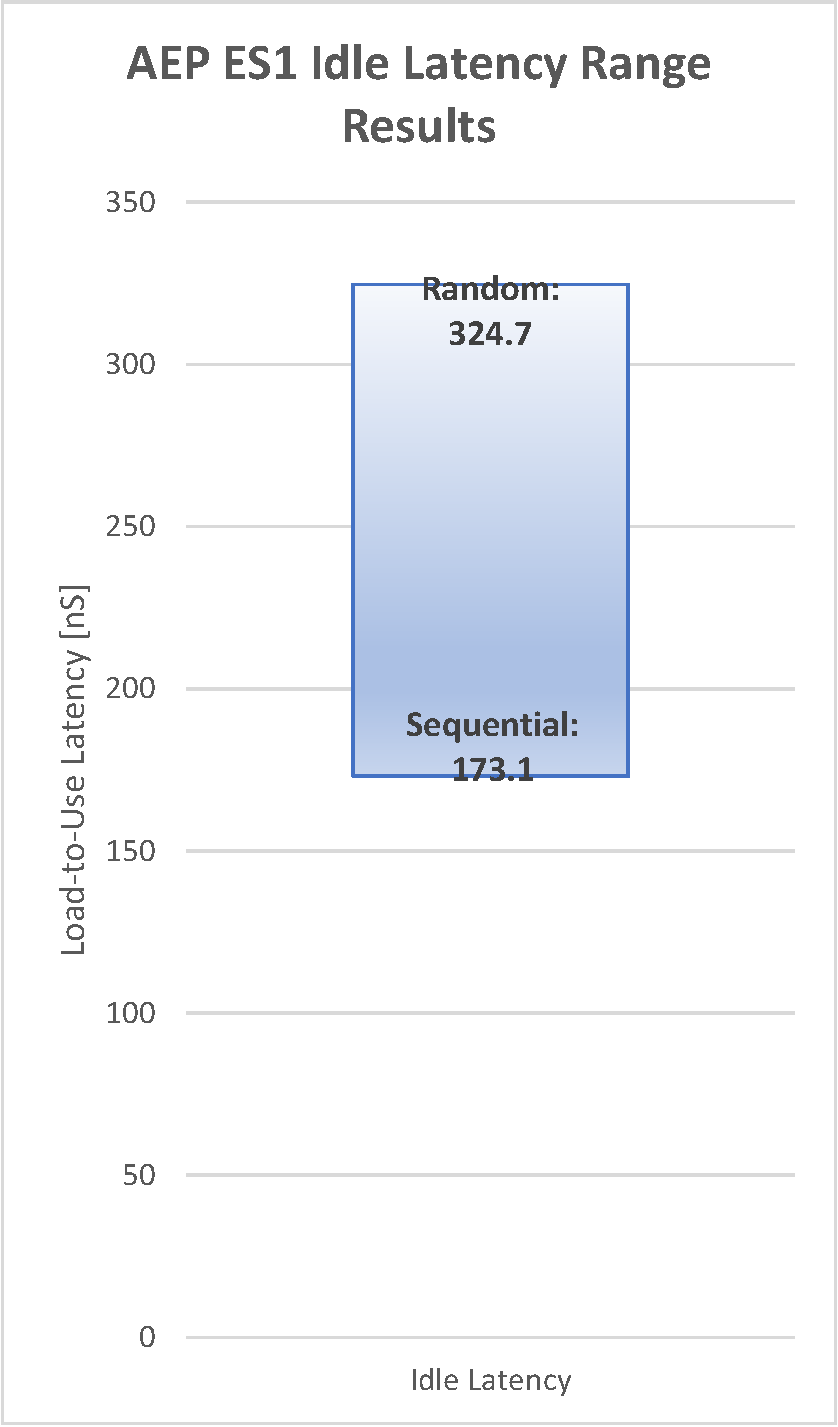
\includegraphics[scale=0.5]{charts/aep_eval_idle_latency-crop.pdf}
\end{figure}

\begin{figure}
    \centering
    \caption{Random Read Load Latency Evaluation of Test System against Intel Reference}\label{chart:aep:read}
    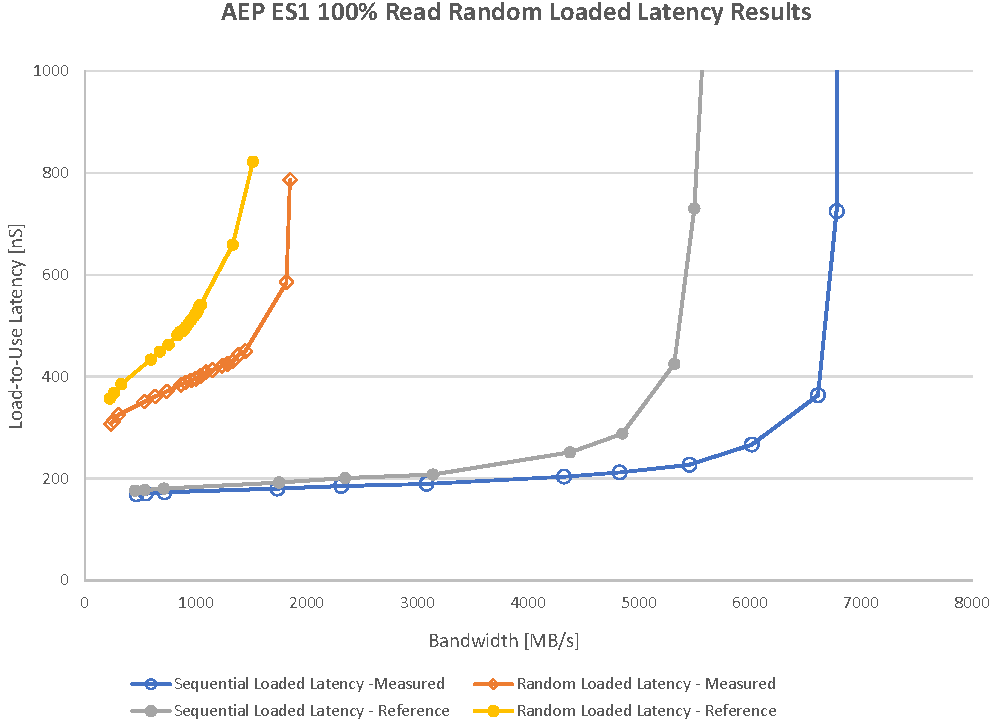
\includegraphics[scale=0.5]{charts/aep_eval_random_read_load_latency-crop.pdf}
\end{figure}

\begin{table}
    \centering
    \caption{Test System versus Intel Reference}\label{mlc:reference}
    \begin{tabular}{@{}cl@{}}
        Test Description & Figure \\ \toprule
        Idle Memory Latency & \ref{chart:aep:idle} \\
        Loaded Memory Bandwidth & \ref{chart:aep:bw} \\
        Random Read Latency & \ref{chart:aep:read} \\ \bottomrule
    \end{tabular}%
\end{table}


Because the early results I was observing were surprising, I spent time to verify that I was
using the tools properly by reproducing the original Intel results.  This exercise was
useful because it allowed me to identify undocumented options being used by Intel in
their own evaluation, understanding how to enable their ``persistent memory'' mode in
the tests, and validate that I was able to obtain comparable results, suggesting that
I was indeed testing the hardware appropriately.  Ultimately, I did adjust my own data
collection techniques to ensure that I was enabling persistent memory mode.

Intel provided benchmark numbers for three tests and the scripts to repeat their tests
on the actual test system. These tests, and the results, are shown in Table \ref{mlc:reference}.
The results were slightly faster, as I was using a newer system, but within 20\% of the original
Intel reference numbers.

\subsection{Non-Temporal Baseline Measurements}


This section describes the information for \textbf{non-temporal move} operations on the same node. Because
these are done as non-temporal move operations, they bypass the cache and write directly to the actual
memory.  Note that the failure domain is discussed in greater detail in \S \ref{section:model:failure}.
The transfer involved here is sufficiently large that the impact of the memory controller caching
does not impact behavior.

\subsubsection{DRAM}\label{baseline:dram}

\begin{figure}
    \centering
    \caption{Baseline Measurement of DRAM Non-Temporal Write on the same NUMA Node}\label{chart:baseline:dram}
    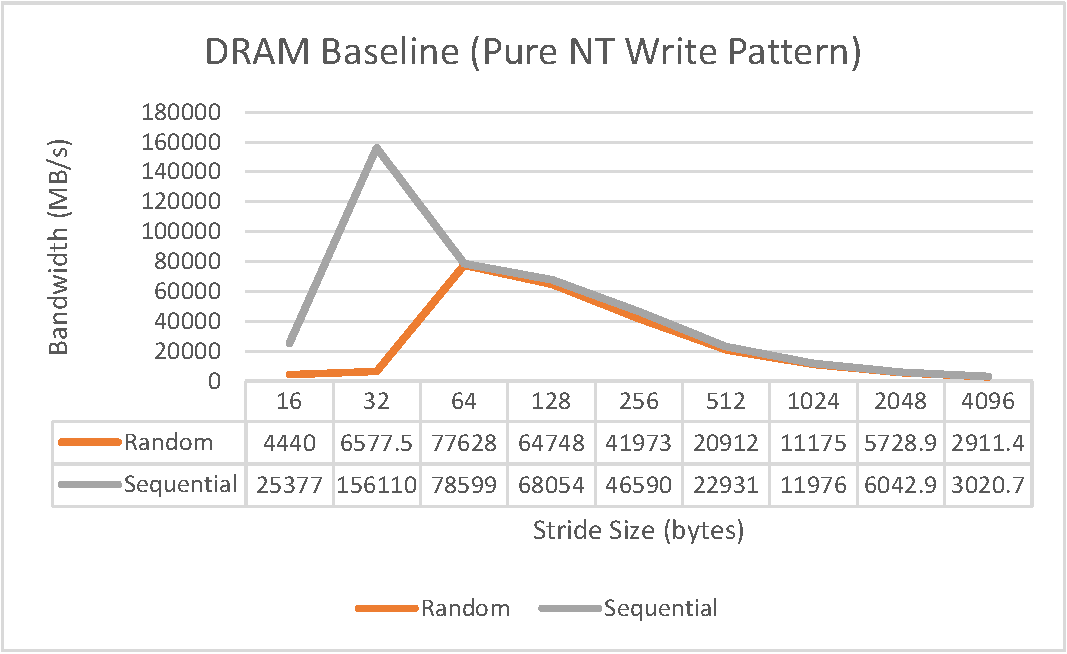
\includegraphics[width=1\textwidth]{charts/dram-baseline-nt-write-same-node-crop.pdf}
\end{figure}

Baseline testing was done using the switches:

\begin{verbatim}
    --loaded_latency -d0 -t10 -W6 -l1024 -T 
        -odata/bw_ctl_pmem0p1_seq_W6-0_23_400000_dram.dat
\end{verbatim}

The file \verb+data/bw_ctl_pmem0p1_seq_W6-0_23_400000_dram.dat+ contained the confirmation information
for the specific test layout:

\begin{verbatim}
0       W6 seq 400000 dram 0
1-23    W6 seq 400000 dram 0
\end{verbatim}

This drives the test to use core 0 for latency measurements, and cores 1-23 for load generation.

Note that the \verb+-l+ option was varied depending upon the ``stride'' size (unit of data handling).
The control file specified the disposition of the individual CPUs

I do not report results for any other DRAM tests.

Results for this test are showin in Figure \ref{chart:baseline:dram}.

\subsubsection{NVM}\label{baseline:nvm}

\begin{figure}[b]
\centering
    \caption{Baseline Measurement of NVM Non-Temporal Write on the same NUMA Node}\label{chart:baseline:nvm}
    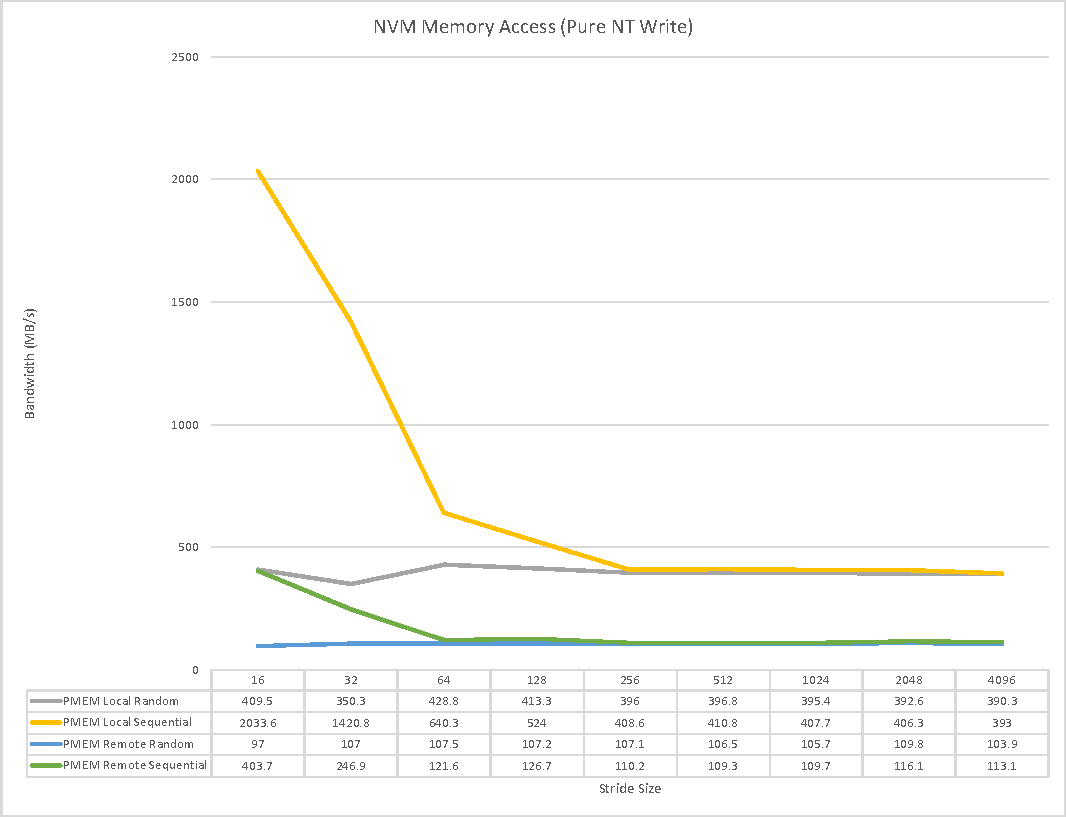
\includegraphics[width=1\textwidth]{charts/nt-write-both-nodes-crop.pdf}
\end{figure}

Baseline testing was done using the switches:

\begin{verbatim}
    --loaded_latency -d0 -t10 -W6 -l64 \
      -odata/bw_ctl_pmem0p1_seq_W6-0_23_400000_pmem.dat}
\end{verbatim}

The file \verb+data/bw_ctl_pmem0p1_seq_W6-0_23_400000_dram.dat+ contained the confirmation information
for the specific test layout:

\begin{verbatim}
0    W6 seq 400000 pmem /mnt/pmem0p1
1-23 W6 seq 400000 pmem /mnt/pmem0p1
\end{verbatim}

The \verb+pmem+ directive is used to put the test utility into ``persistent memory'' testing mode.
The final value is the name of the directory to use.  It \textbf{must} be a persistent memory
to run this test.  Otherwise the test will refuse to run.


\subsection{Cached Read}\label{mlc:r}

\subsubsection{Random Read}
\begin{figure}
    \centering
    \caption{Random Read (R)}\label{chart:random:read}
    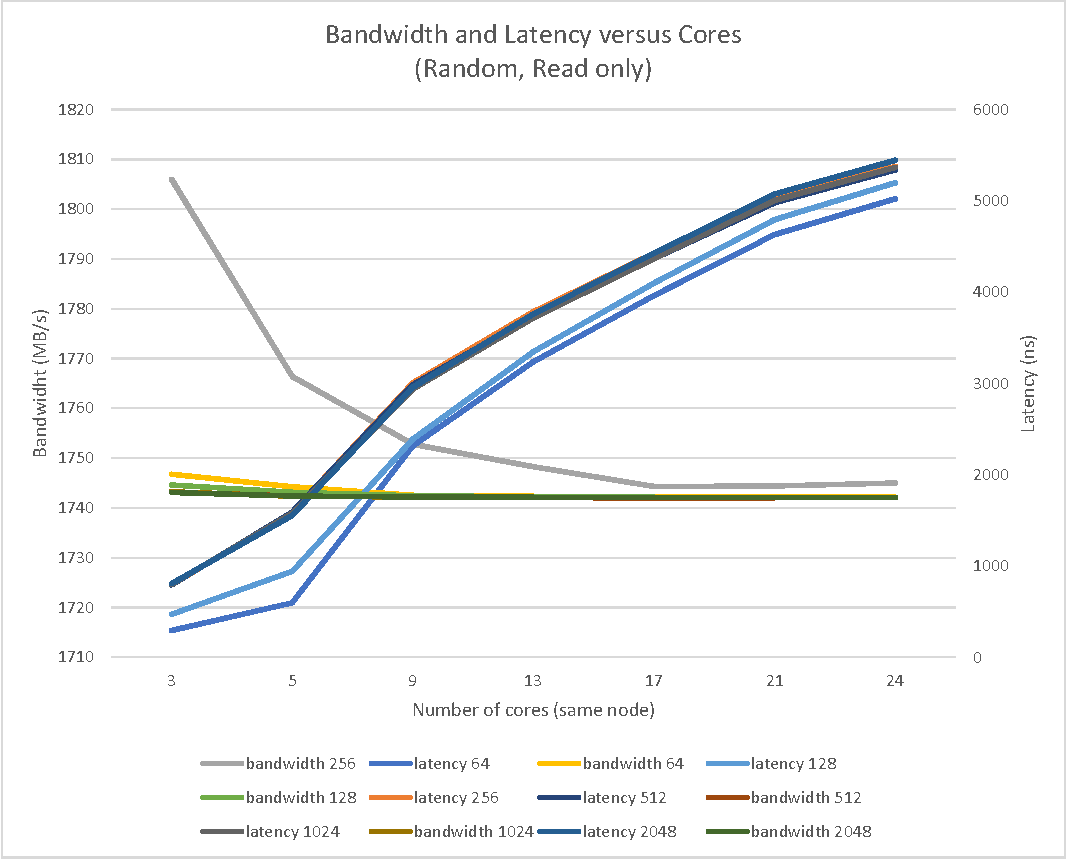
\includegraphics[scale=0.5]{charts/random-r-crop.pdf}
\end{figure}

\begin{figure}
    \centering
    \caption{Sequential Read (R)}\label{chart:sequential:read}
    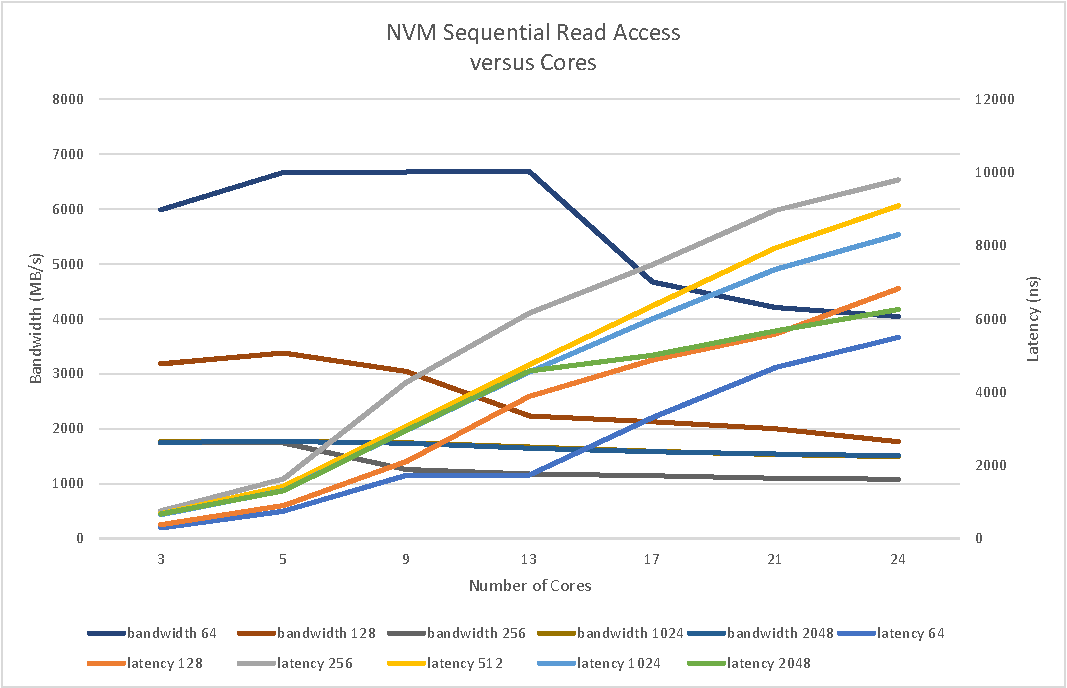
\includegraphics[scale=0.5]{charts/sequential-r-crop.pdf}
\end{figure}

\begin{figure}
    \centering
    \caption{Random 2:1 Read/Write (W2)}\label{chart:random:W2}
    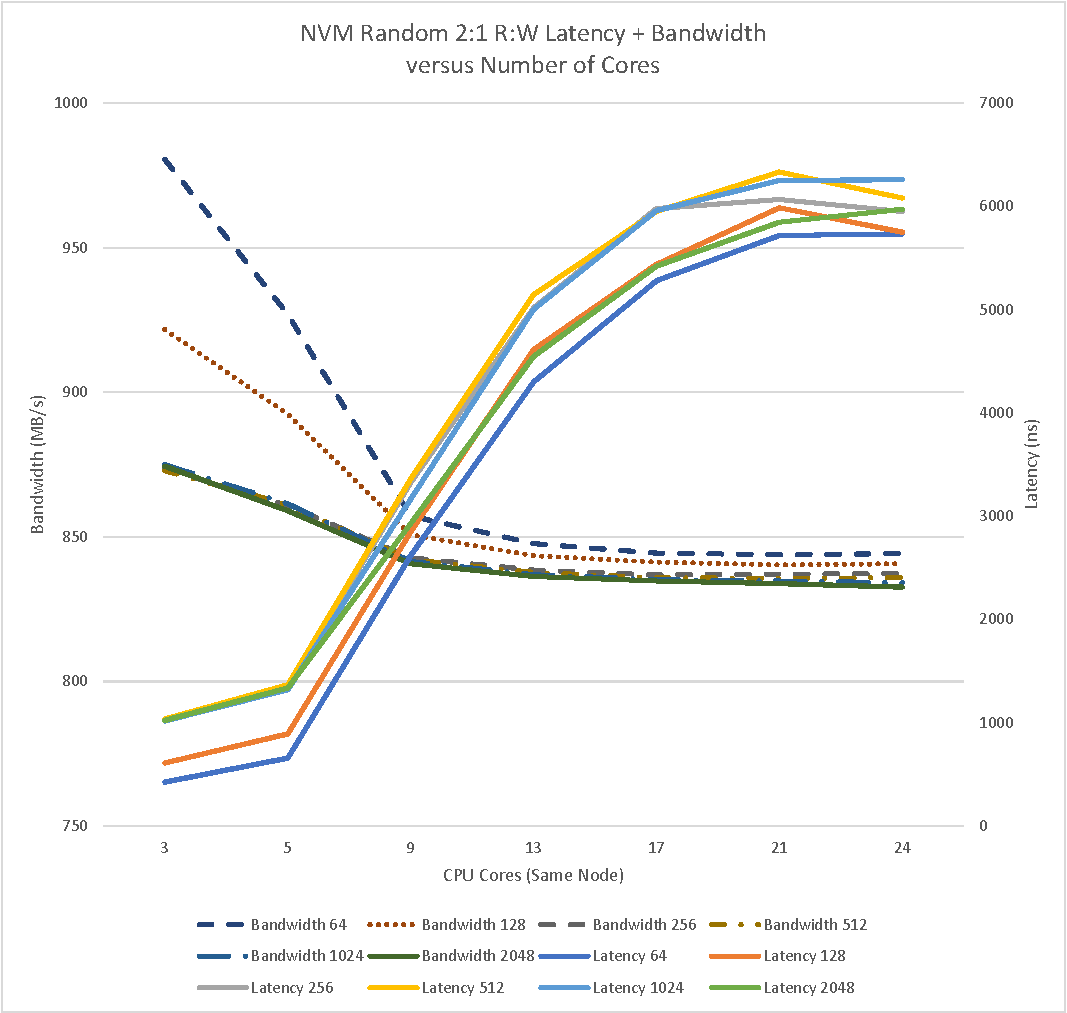
\includegraphics[scale=0.5]{charts/random-w2-crop.pdf}
\end{figure}

\begin{figure}
    \centering
    \caption{Sequential 2:1 Read/Write (W2)}\label{chart:sequential:W2}
    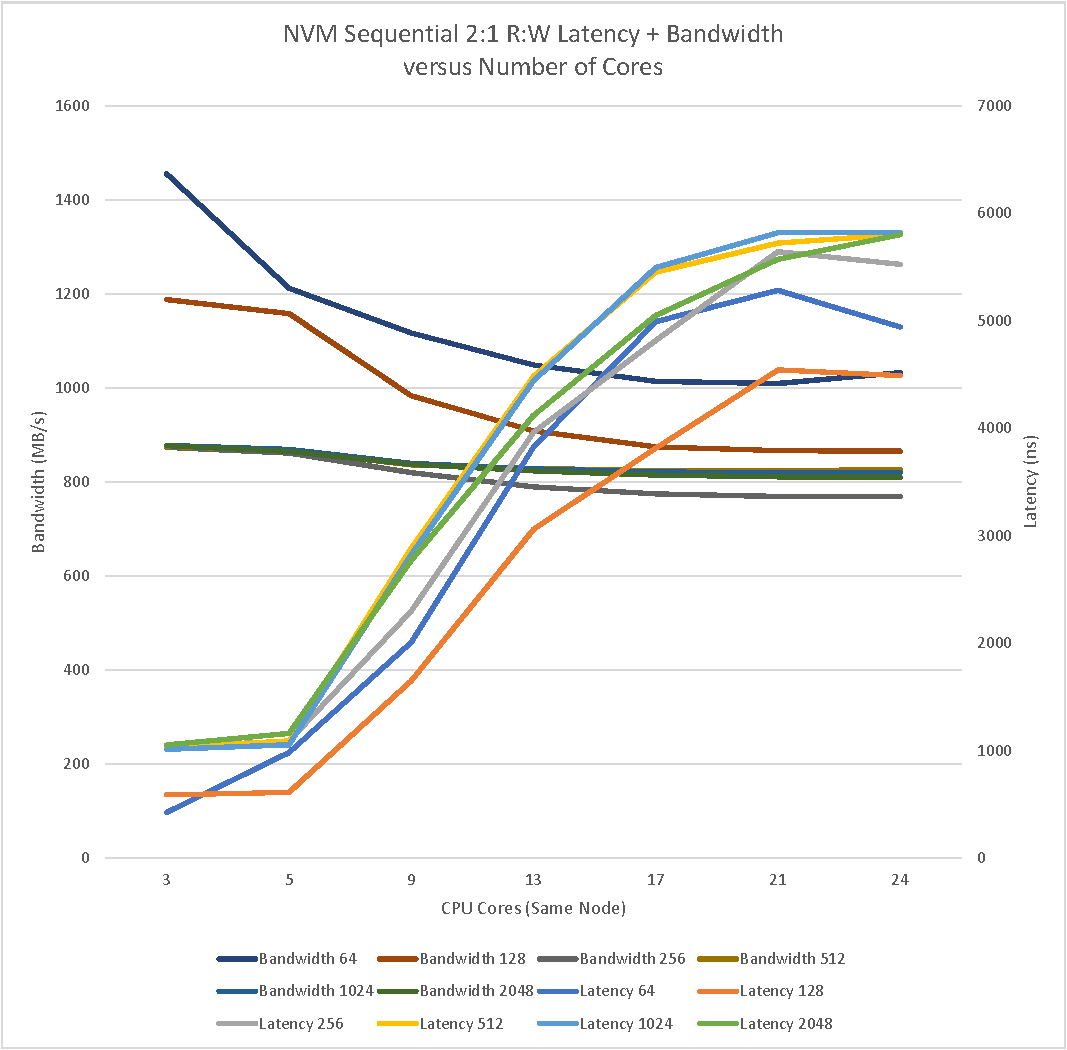
\includegraphics[scale=0.5]{charts/sequential-w2-crop.pdf}
\end{figure}

\begin{figure}
    {\centering
    \caption{Sequential 3:1 Read/Write (W3)}\label{chart:sequential:w3}
    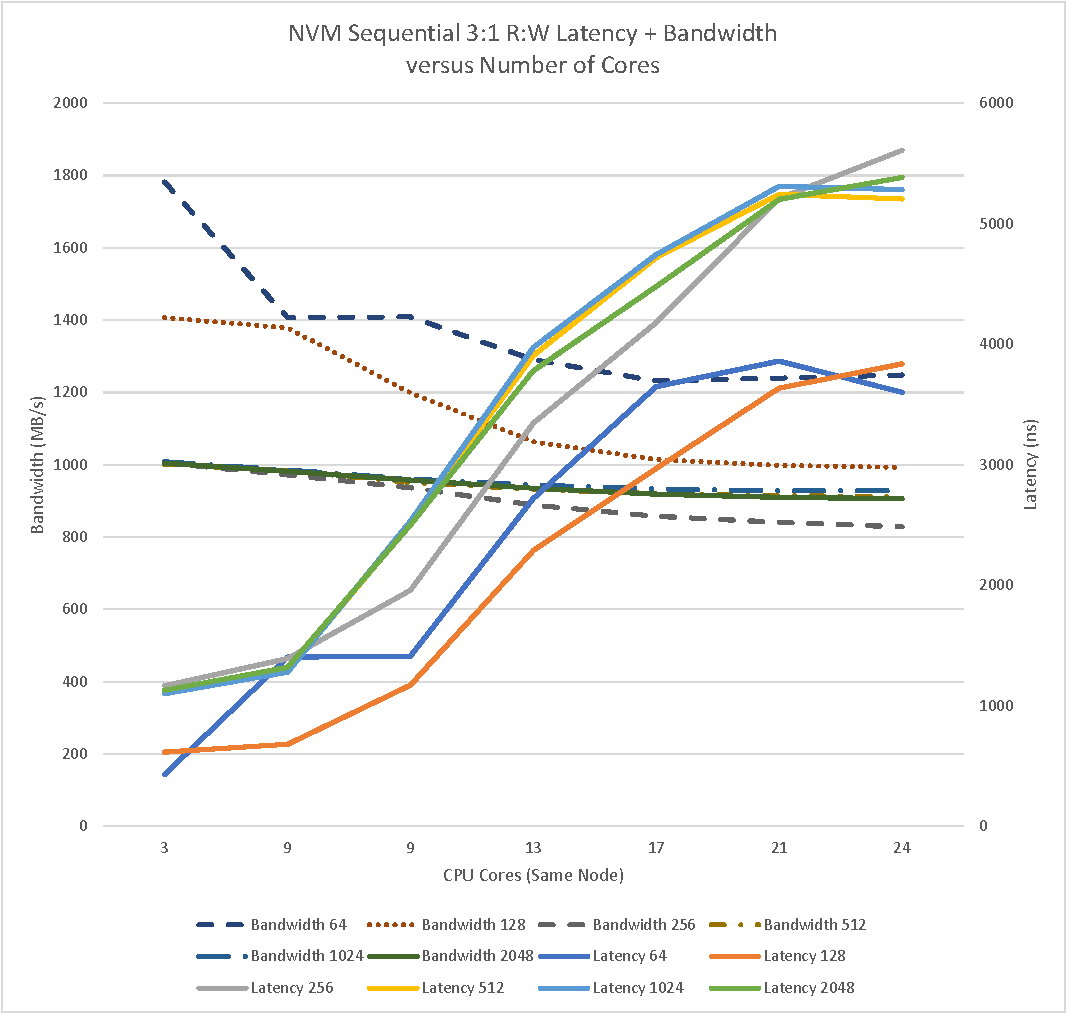
\includegraphics[scale=0.5]{charts/sequential-w3-crop.pdf}
    }
\end{figure}



\begin{figure}
    \centering
    \caption{Random 1:1 Read/Write (W5)}\label{chart:random:W5}
    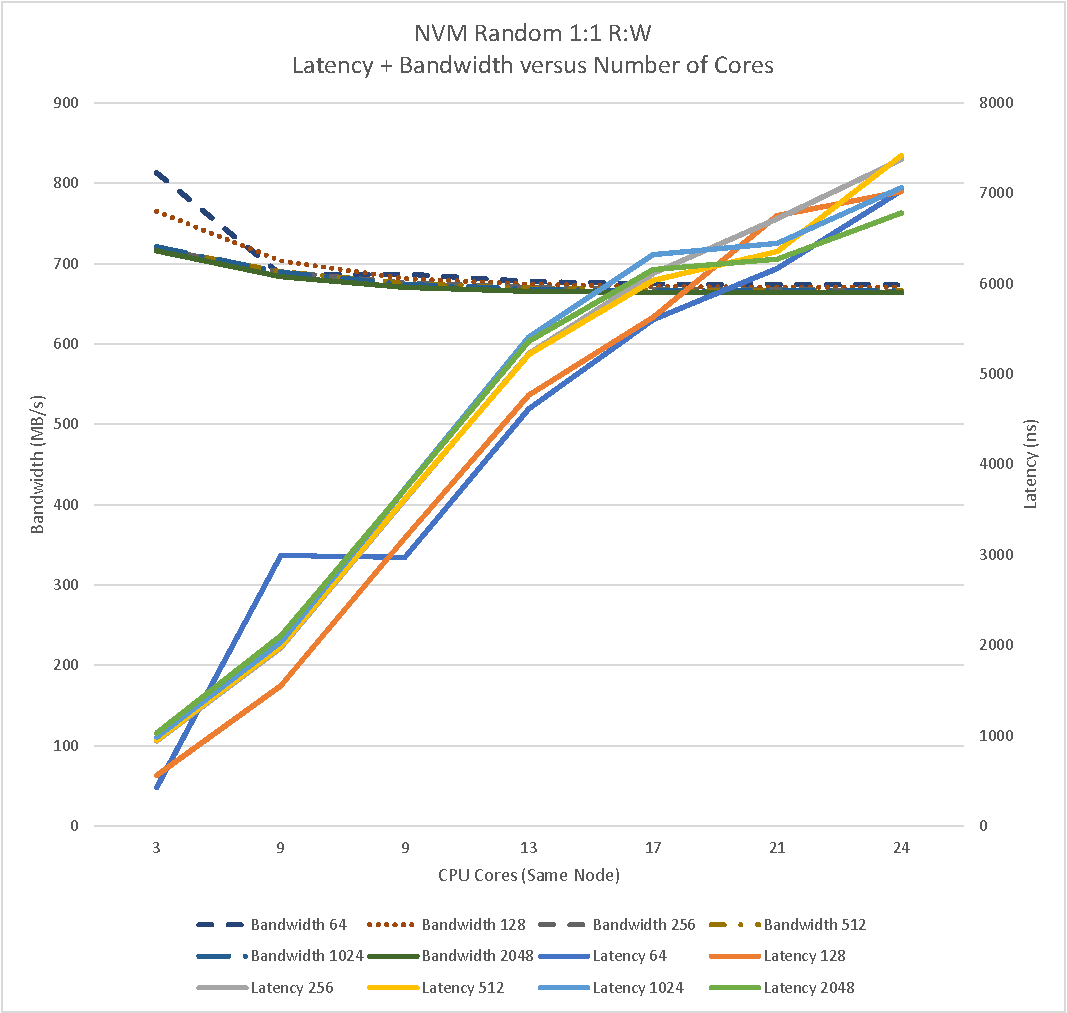
\includegraphics[scale=0.5]{charts/random-w5-crop.pdf}
\end{figure}





\begin{figure}
    \centering
    \caption{Random Non-Temporal Write (W6)}\label{chart:random:w6}
    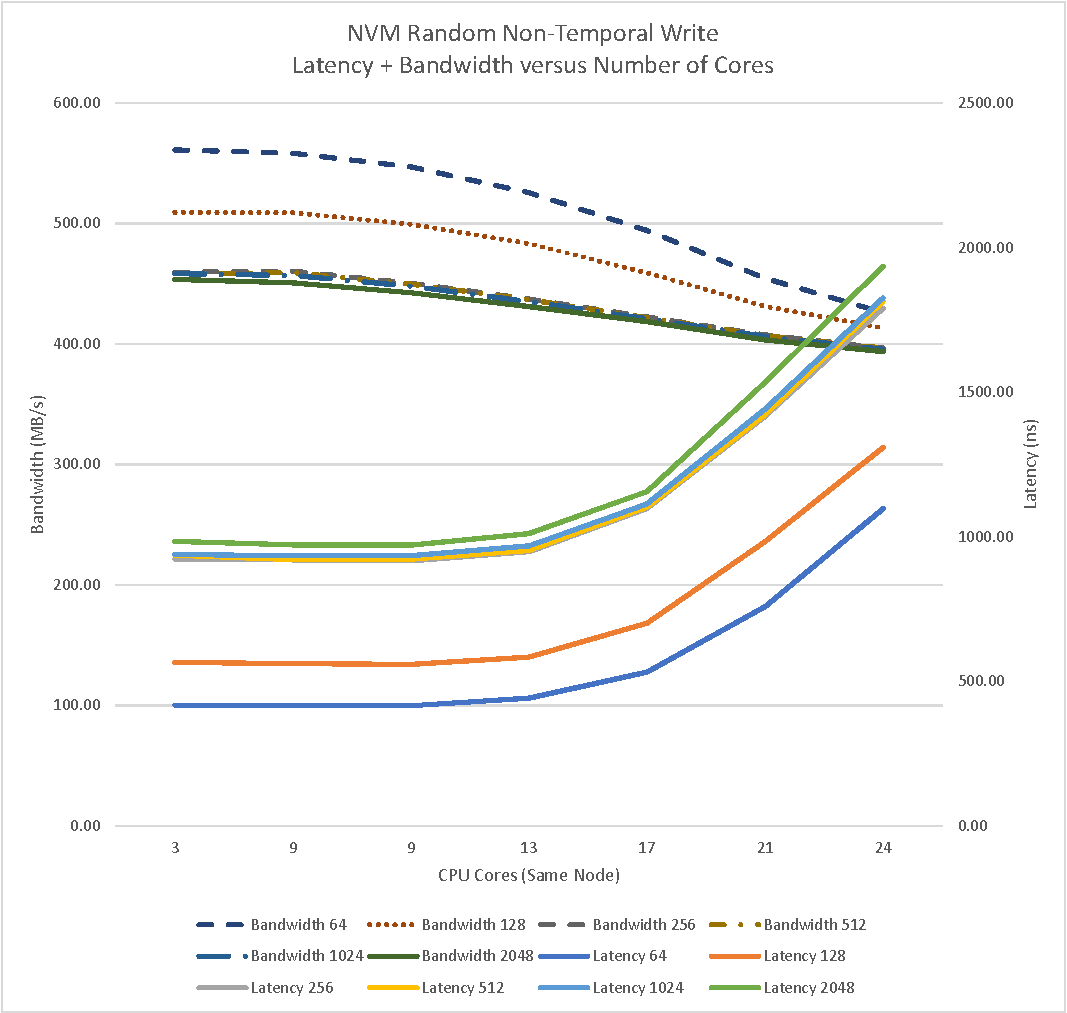
\includegraphics[scale=0.5]{charts/random-w6-crop.pdf}
\end{figure}

\begin{figure}
    \centering
    \caption{Random 2:1 Read to Non-Temporal Write (W7)}\label{chart:random:W7}
    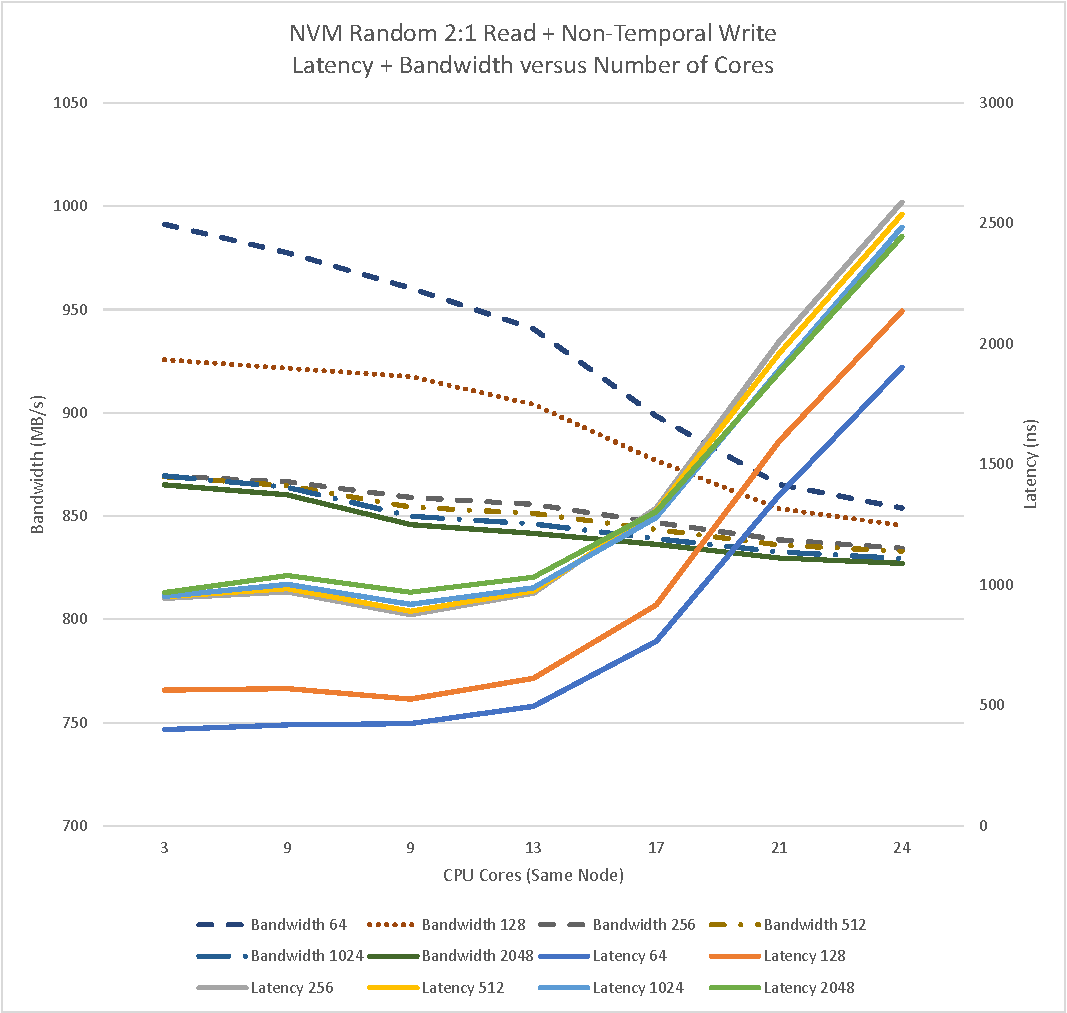
\includegraphics[scale=0.5]{charts/random-w7-crop.pdf}
\end{figure}

\begin{figure}
    \centering
    \caption{Random 1:1 Read to Non-Temporal Write (W8)}\label{chart:random:W8}
    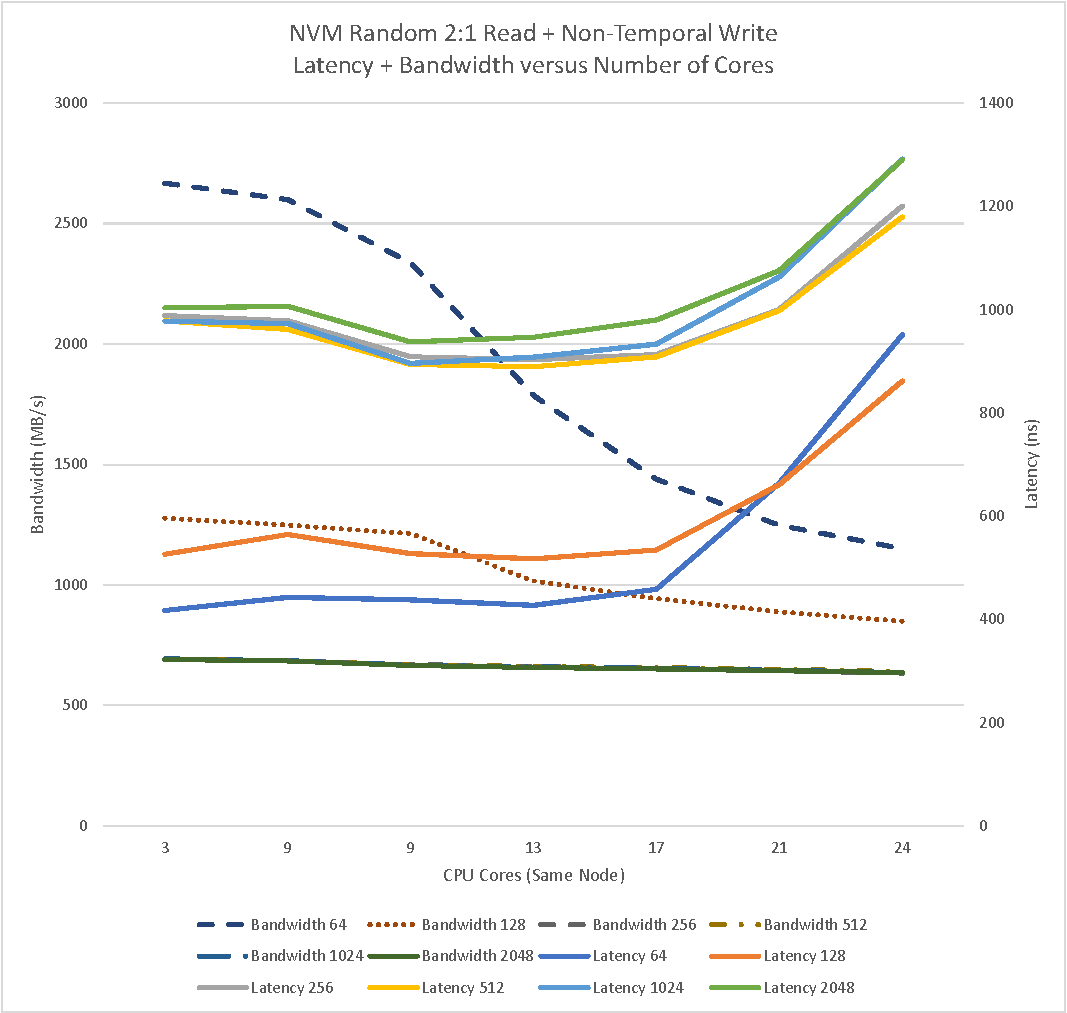
\includegraphics[scale=0.5]{charts/random-w8-crop.pdf}
\end{figure}

\begin{figure}
    \centering
    \caption{Sequential 1:1 Read to Write (W5)}\label{chart:sequential:W5}
    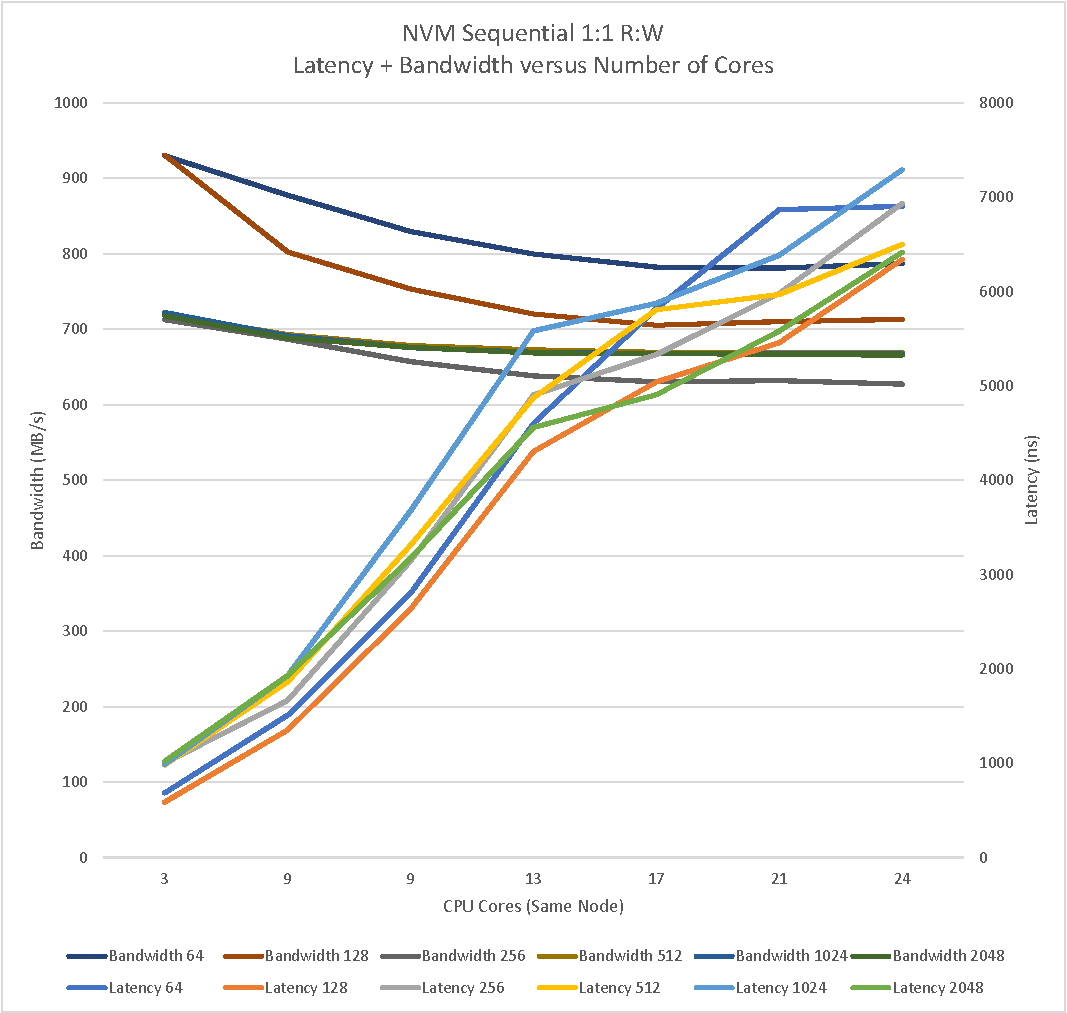
\includegraphics[scale=0.5]{charts/sequential-w5-crop.pdf}
\end{figure}


\begin{figure}
    \centering
    \caption{Sequential Non-Temporal Write (W6)}\label{chart:sequential:W6}
    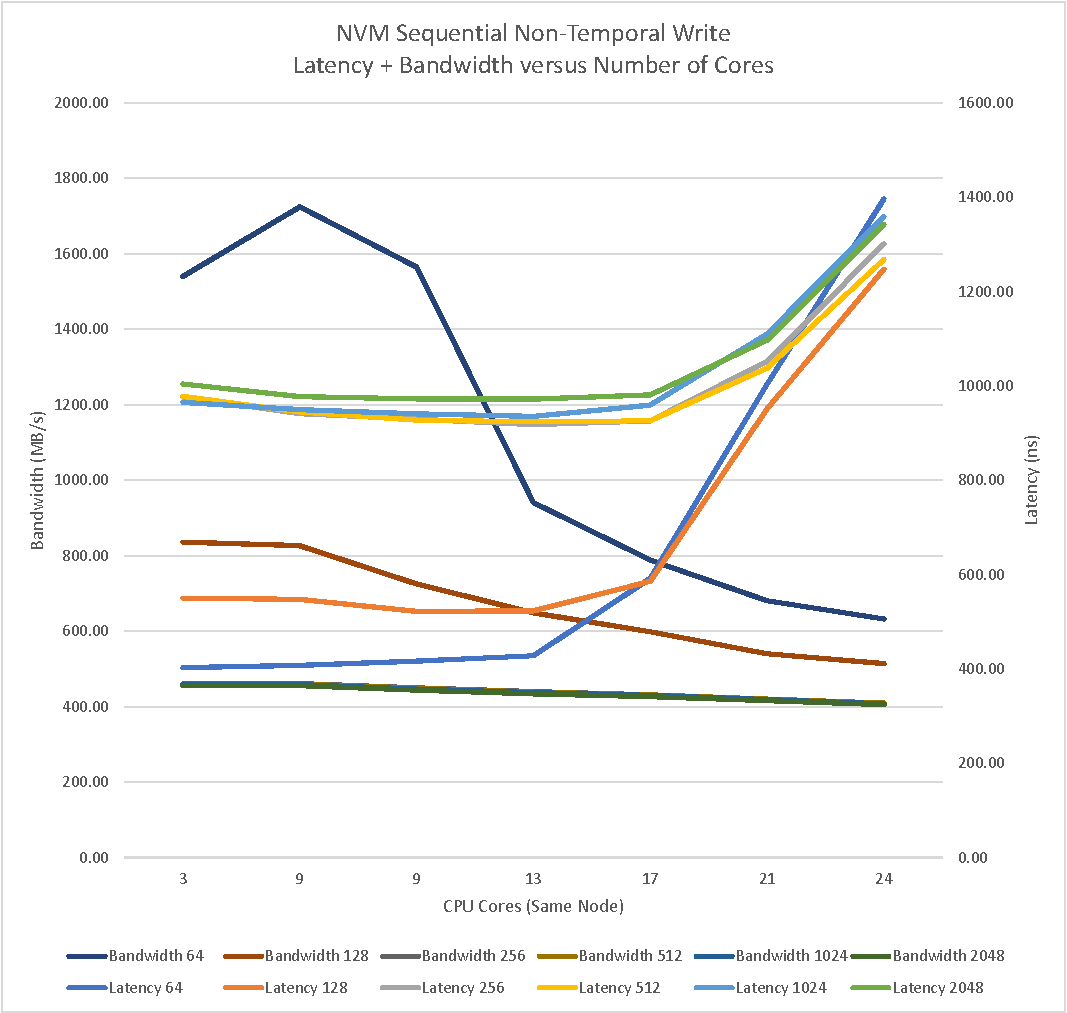
\includegraphics[scale=0.5]{charts/sequential-w6-crop.pdf}
\end{figure}


\begin{figure}
    \centering
    \caption{Sequential 2:1 Read to Non-Temporal Write (W7)}\label{chart:sequential:W7}
    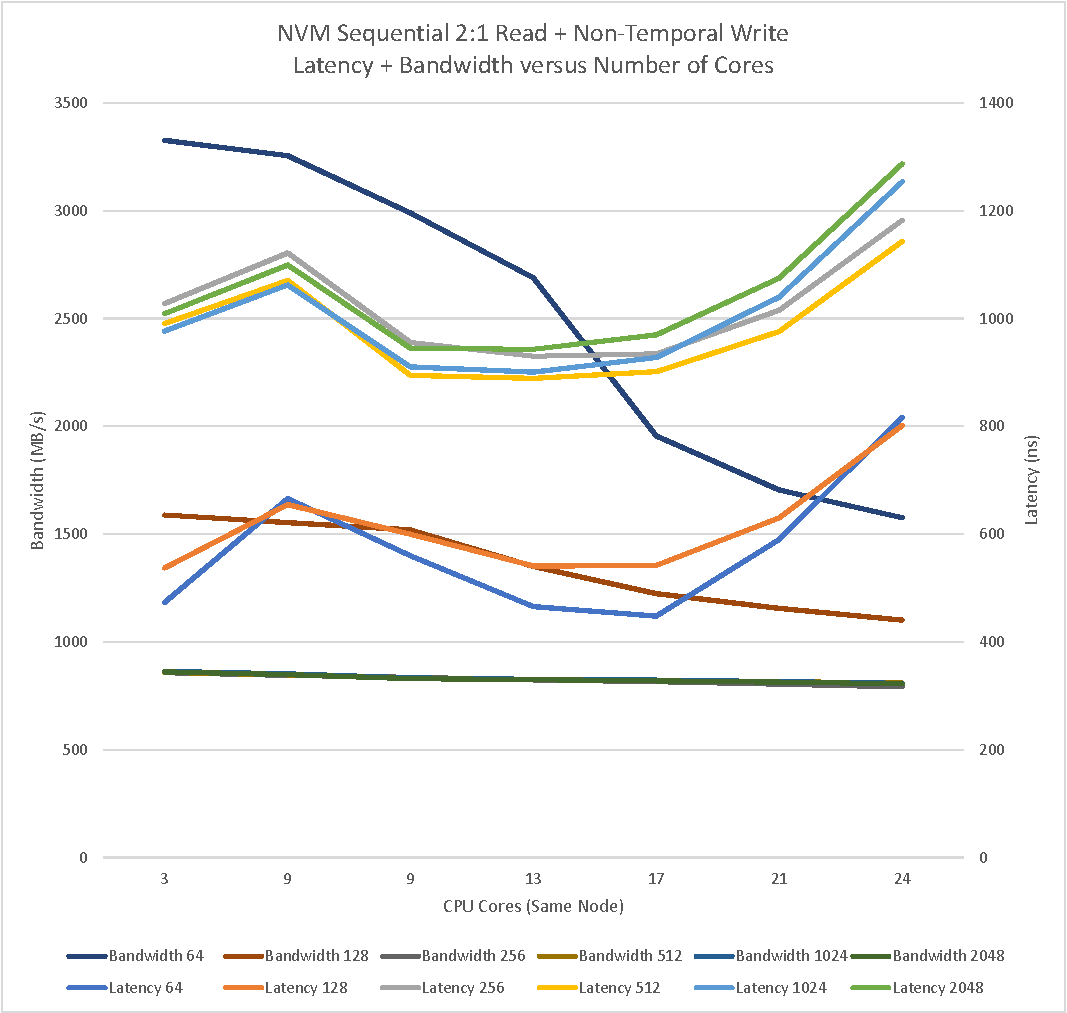
\includegraphics[scale=0.5]{charts/sequential-w7-crop.pdf}
\end{figure}


\begin{figure}
    \centering
    \caption{Sequential 3:1 Read to Non-Temporal Write (streaming triad) (W10)}\label{chart:sequential:W10}
    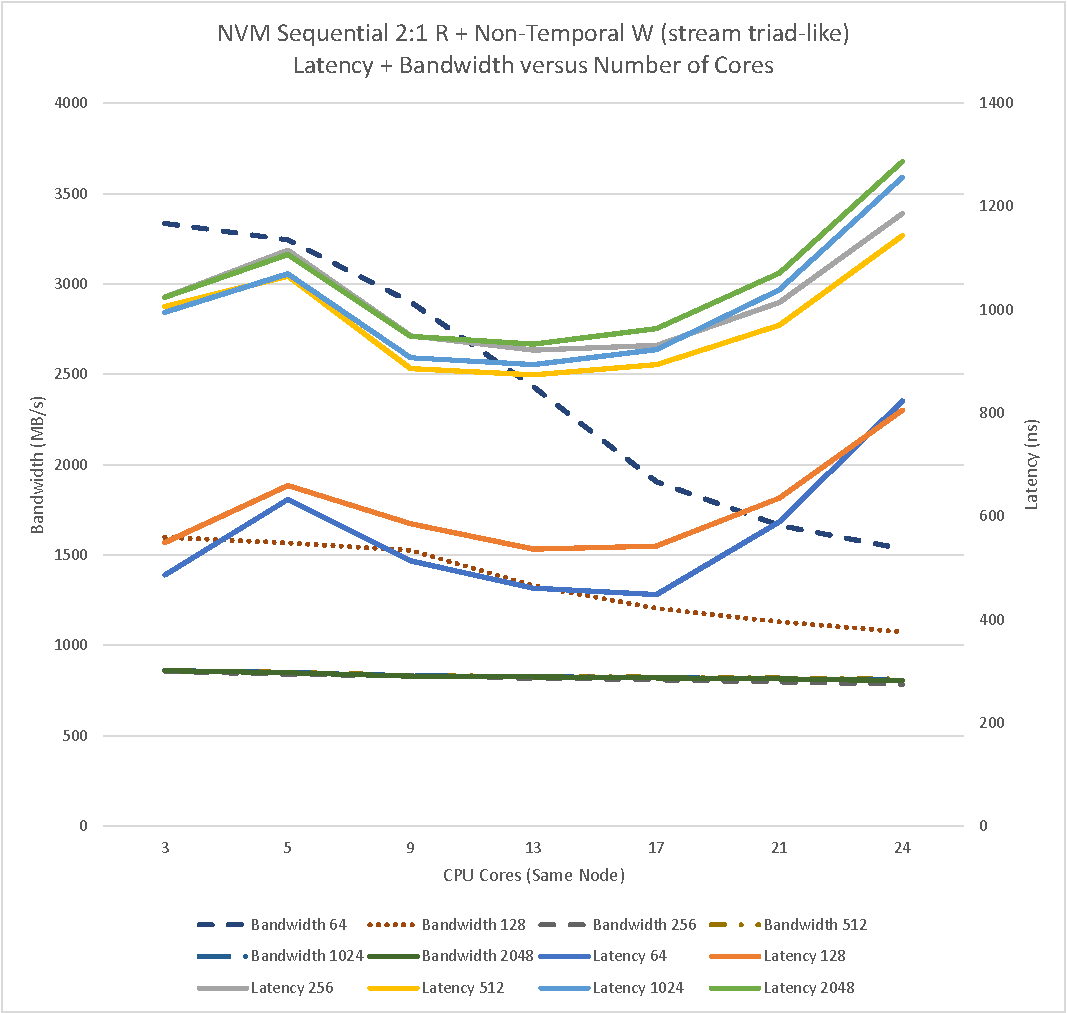
\includegraphics[scale=0.5]{charts/sequential-w10-crop.pdf}
\end{figure}

\section{Micro-Benchmark Results}\label{section:results:micro}

\begin{figure}
    \centering
    \caption{NVM Cache Flush Measurements}\label{micro:cache-flush}
    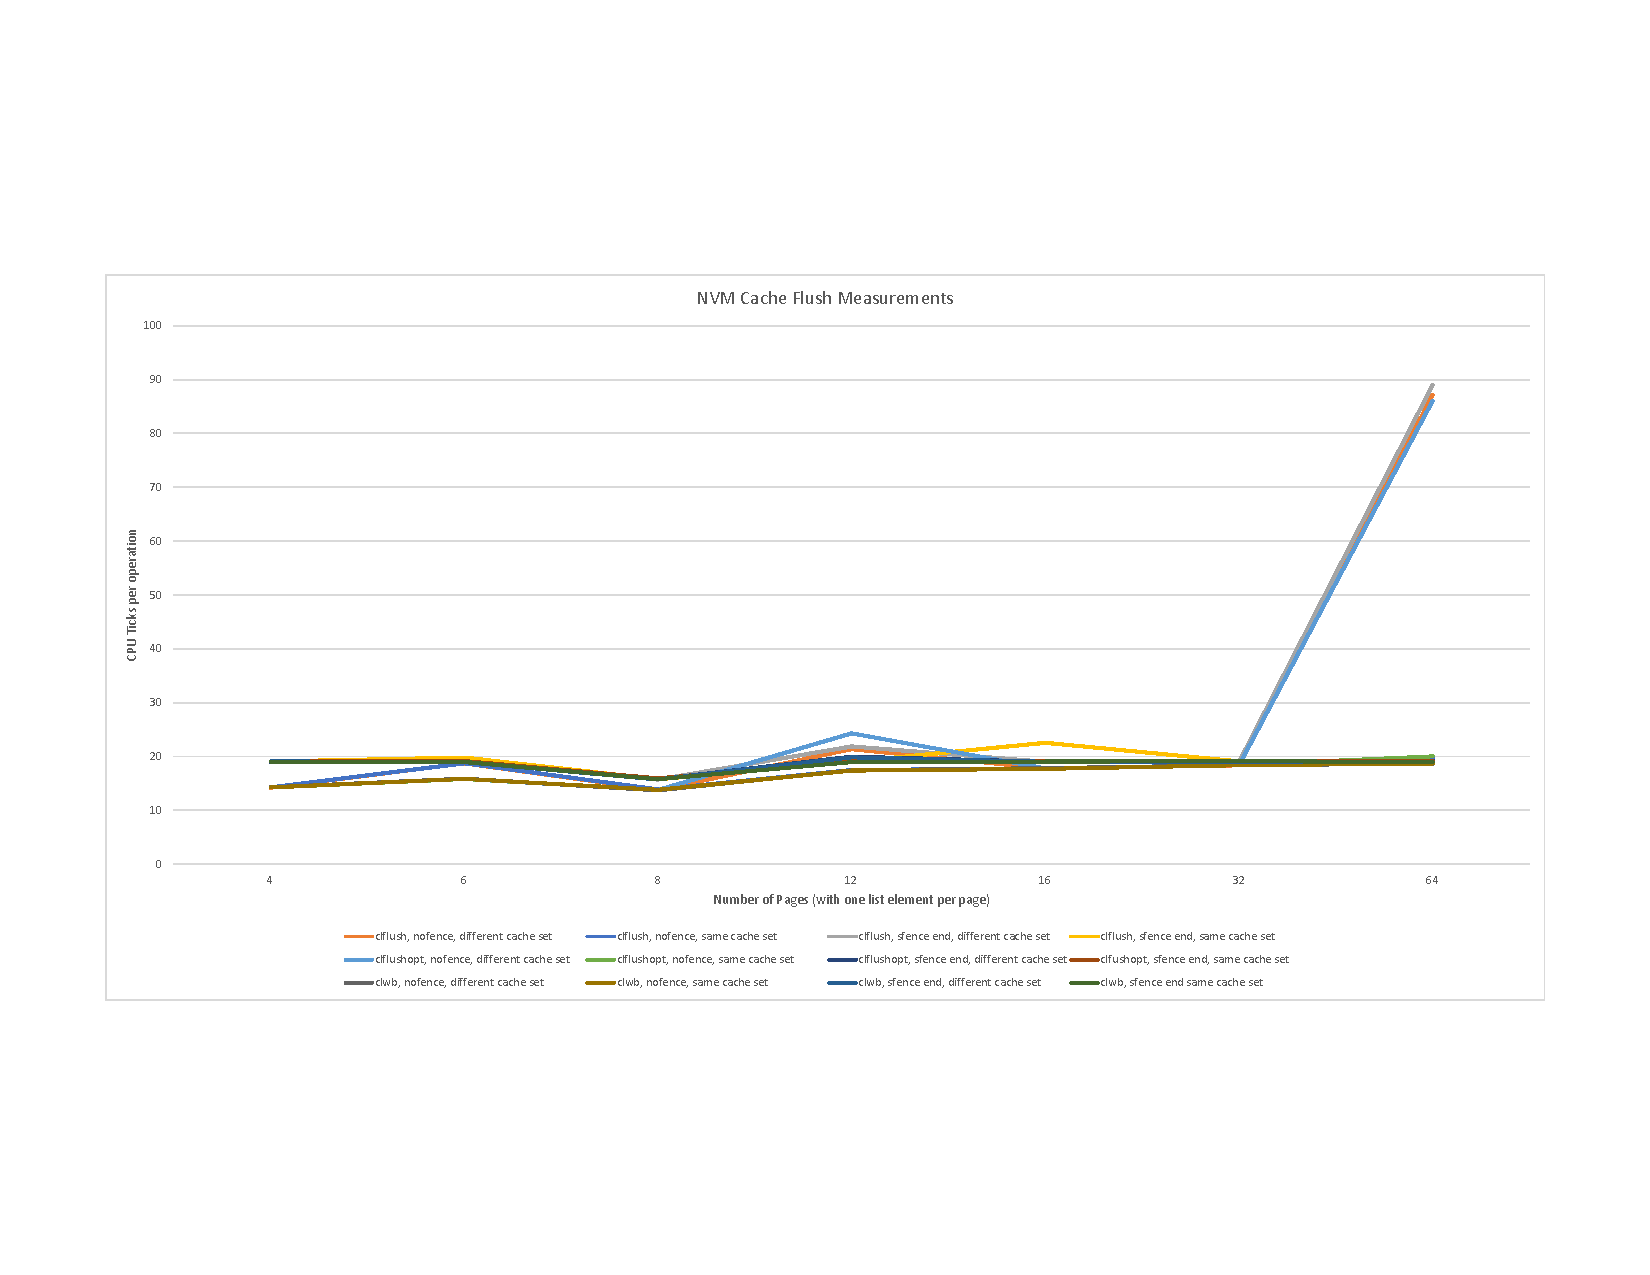
\includegraphics[scale=0.35]{micro/nvm-cache-flush-measurements.pdf}
\end{figure}

\begin{figure}
    \centering
    \caption{NVM CLFLUSHOPT (Different CPU Set)}\label{micro:clflushopt:different}
    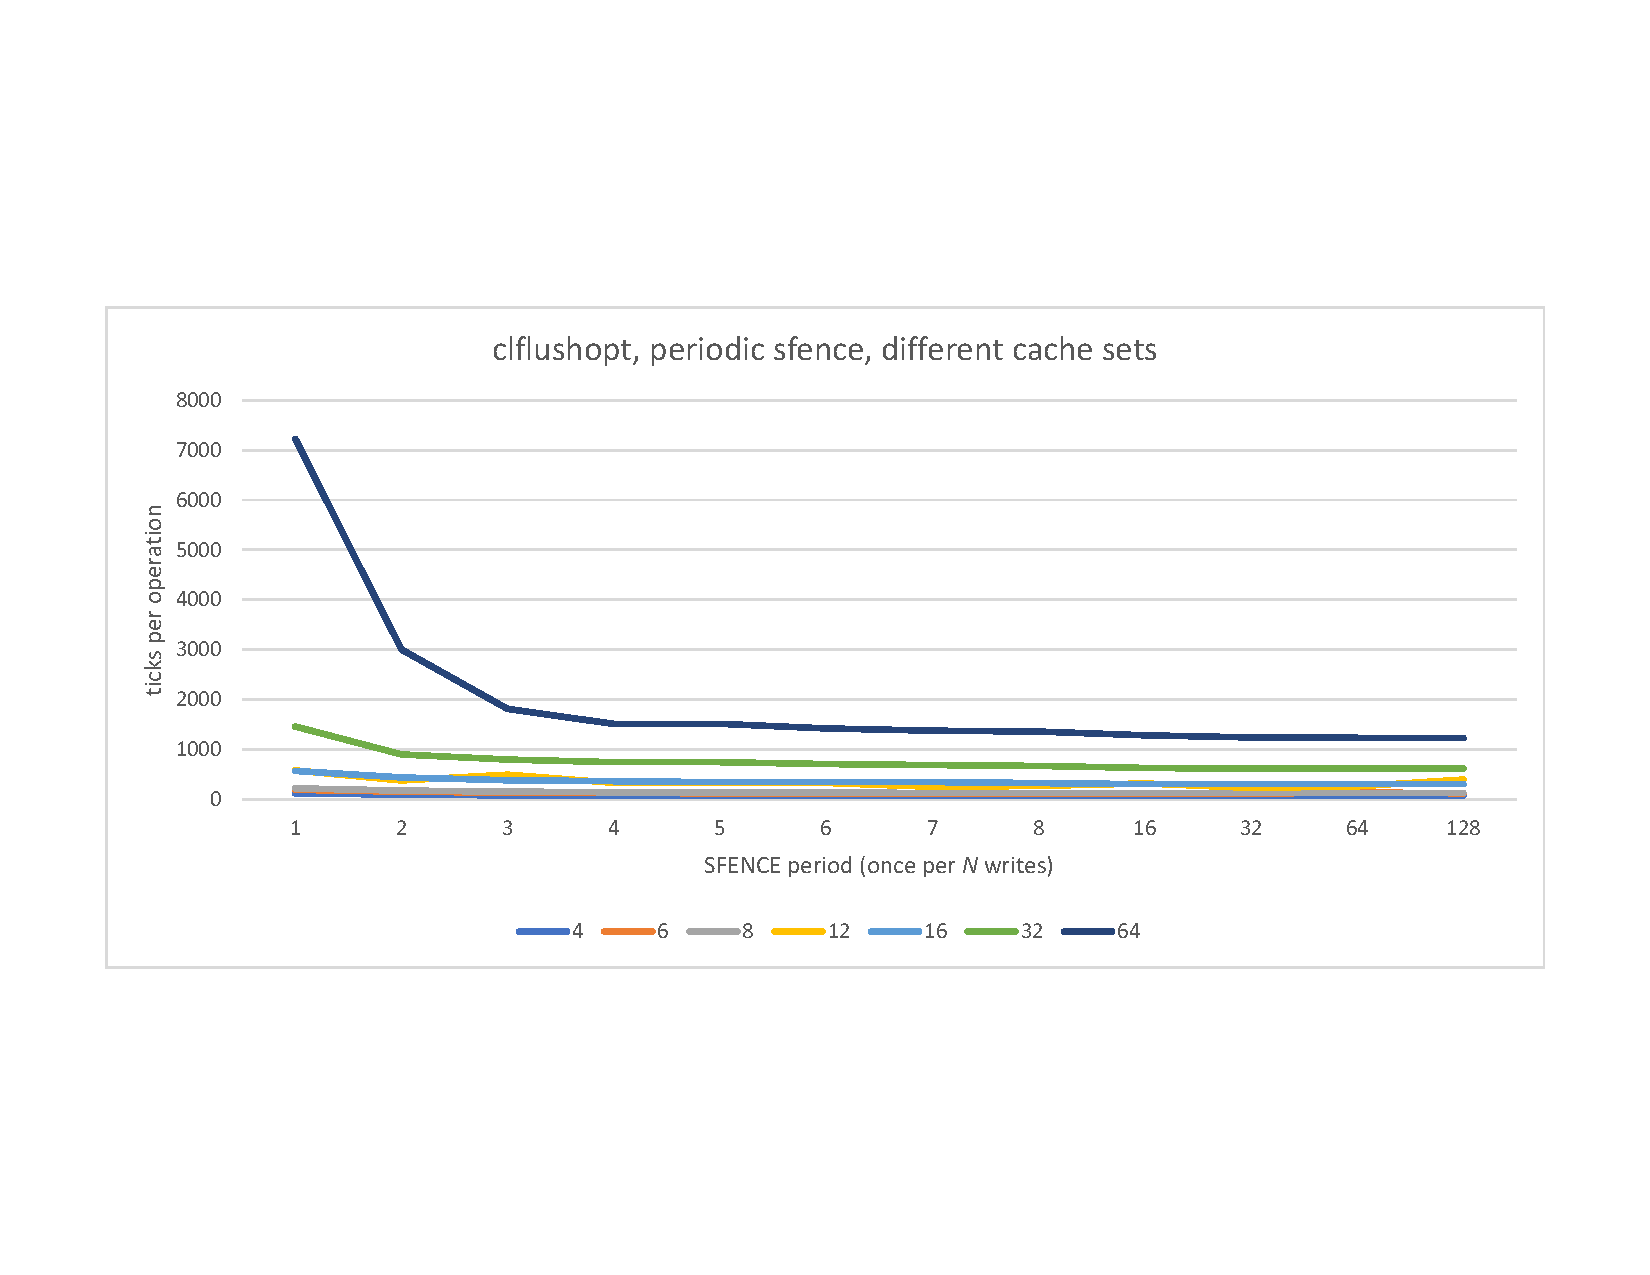
\includegraphics[scale=0.35]{micro/nvm-clflushopt-periodic-different.pdf}
\end{figure}

\begin{figure}
    \centering
    \caption{NVM CLFLUSHOPT (Same CPU Set)}\label{micro:clflushopt:same}
    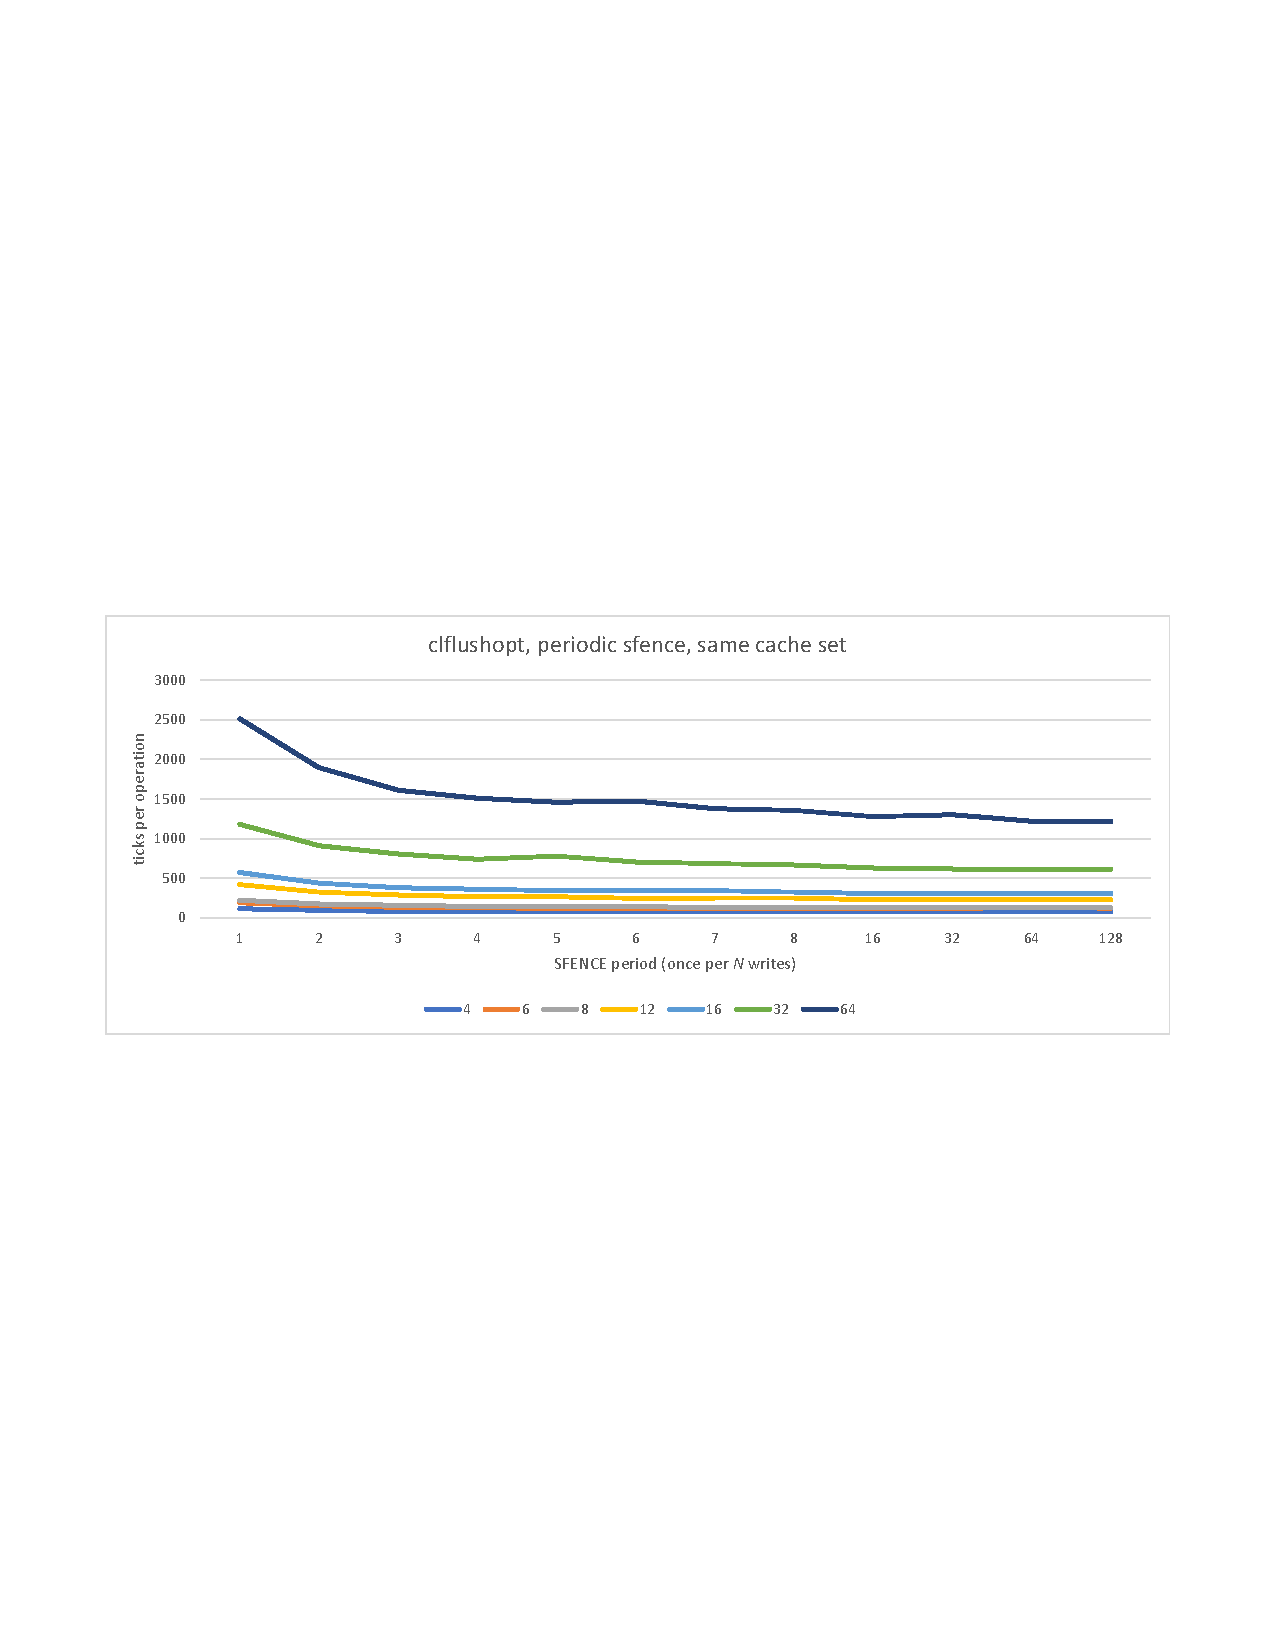
\includegraphics[scale=0.35]{micro/nvm-clflushopt-periodic-same.pdf}
\end{figure}

\begin{figure}
    \centering
    \caption{NVM CLFLUSH (Different CPU Set)}\label{micro:clflush:different}
    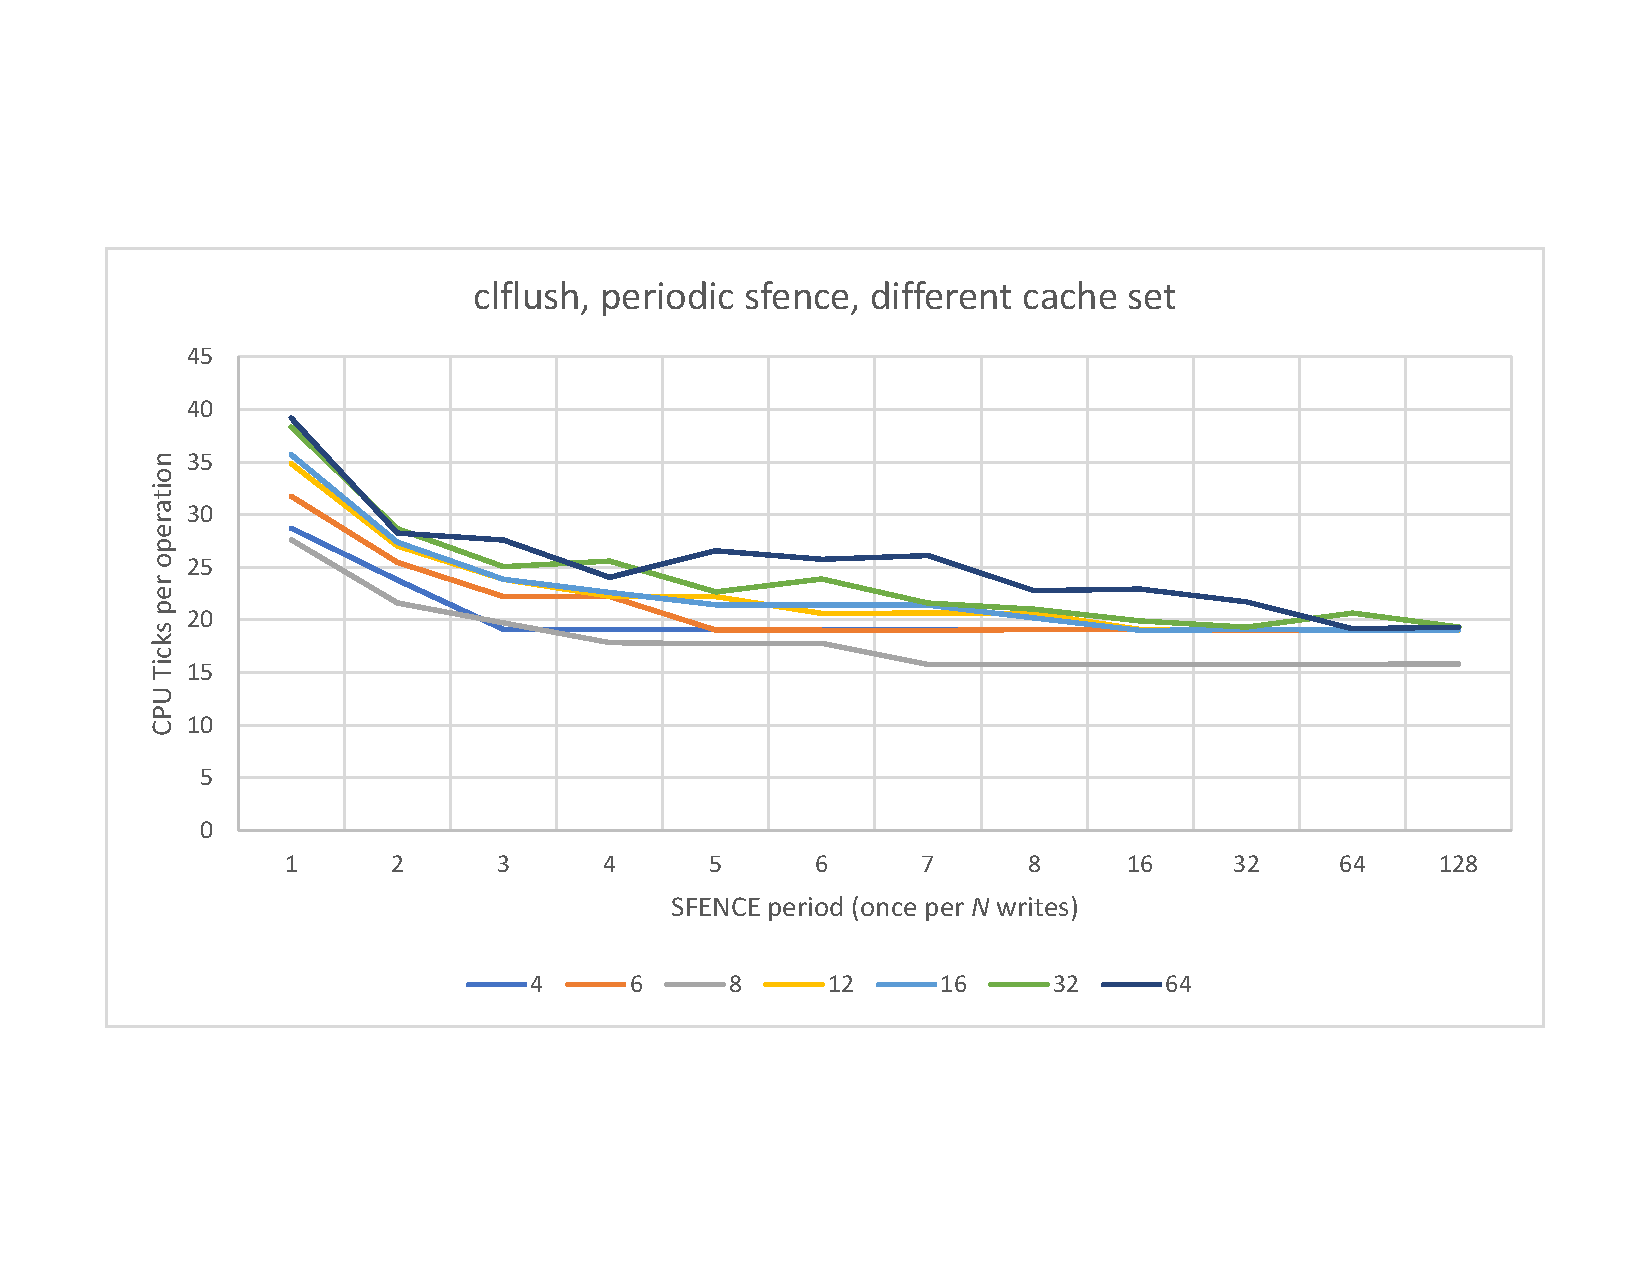
\includegraphics[scale=0.35]{micro/nvm-clflush-periodic-different.pdf}
\end{figure}

\begin{figure}
    \centering
    \caption{NVM CLFLUSH (Same CPU Set)}\label{micro:clflush:same}
    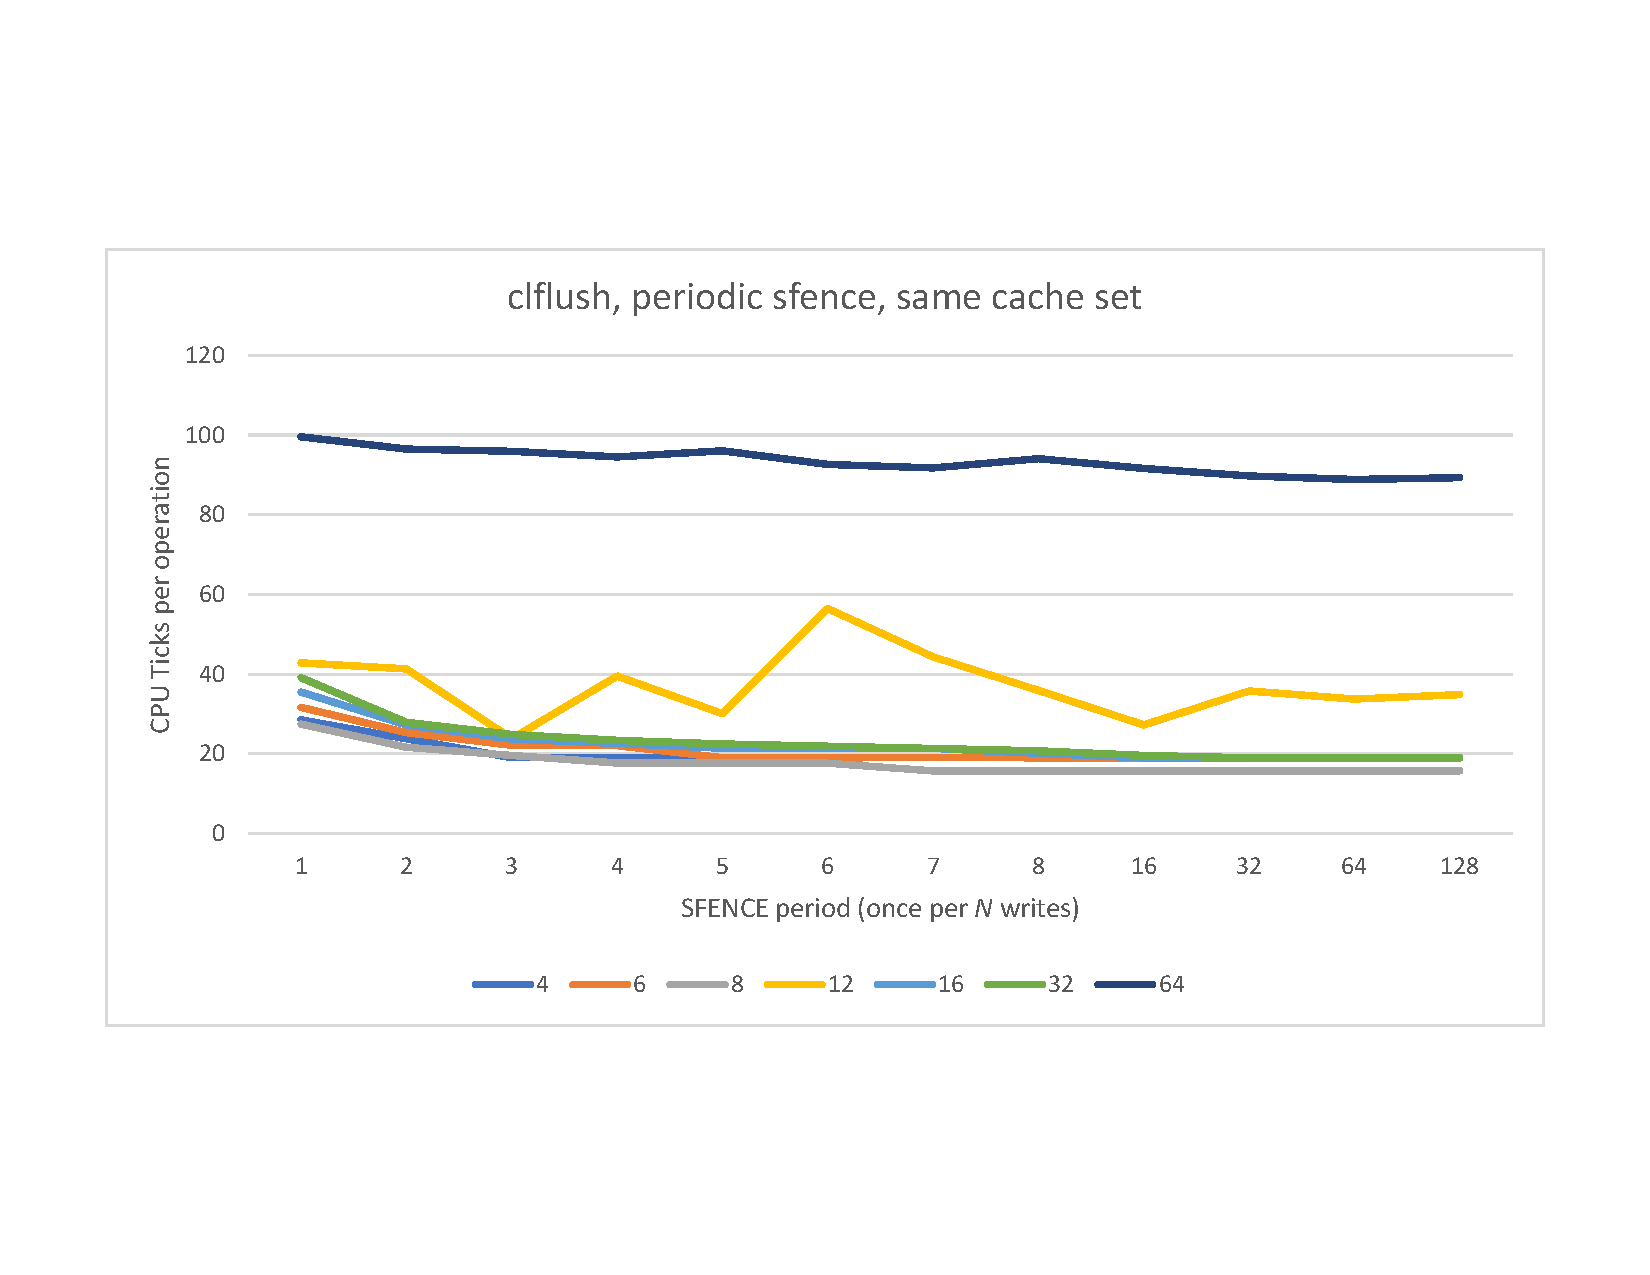
\includegraphics[scale=0.35]{micro/nvm-clflush-periodic-same.pdf}
\end{figure}


\begin{figure}
    \centering
    \caption{NVM CLWB (Different CPU Set)}\label{micro:clwb:different}
    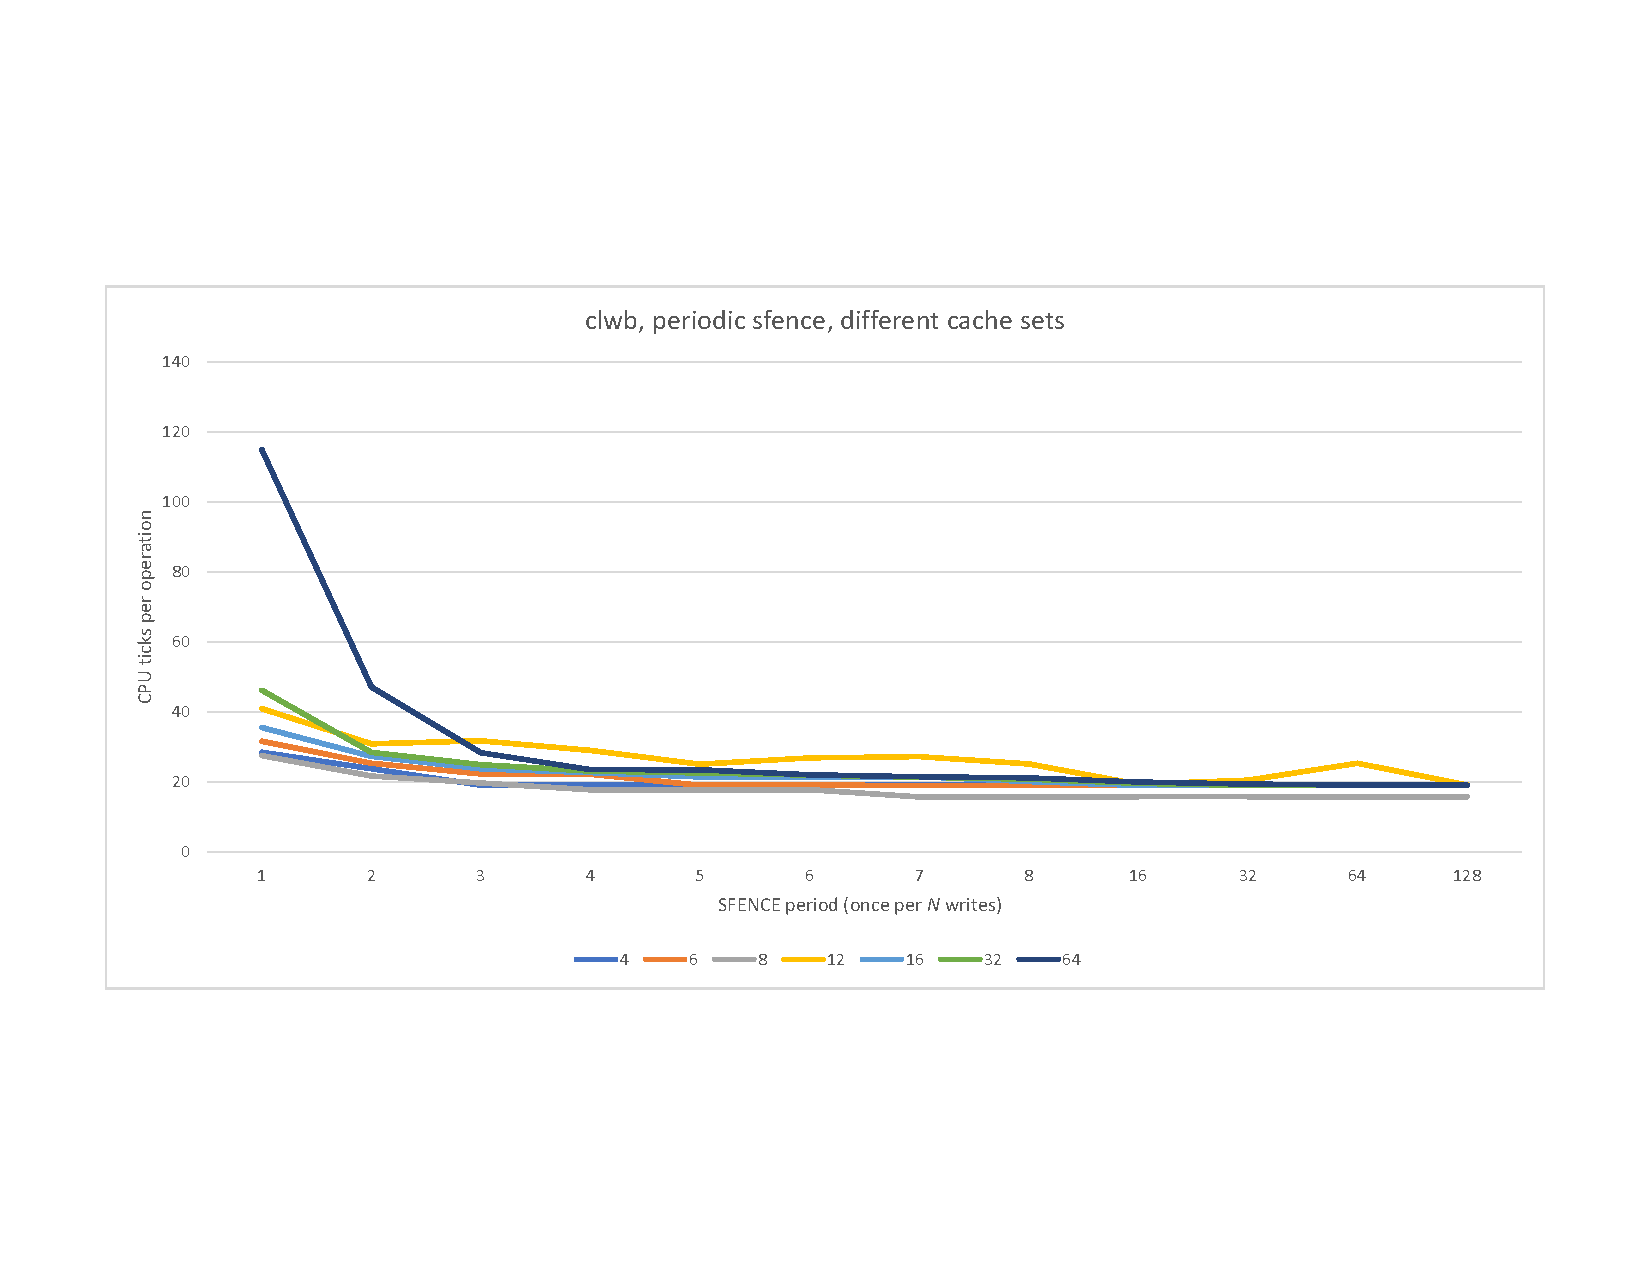
\includegraphics[scale=0.35]{micro/nvm-clwb-periodic-different.pdf}
\end{figure}

\begin{figure}
    \centering
    \caption{NVM CLWB (Same CPU Set)}\label{micro:clwb:same}
    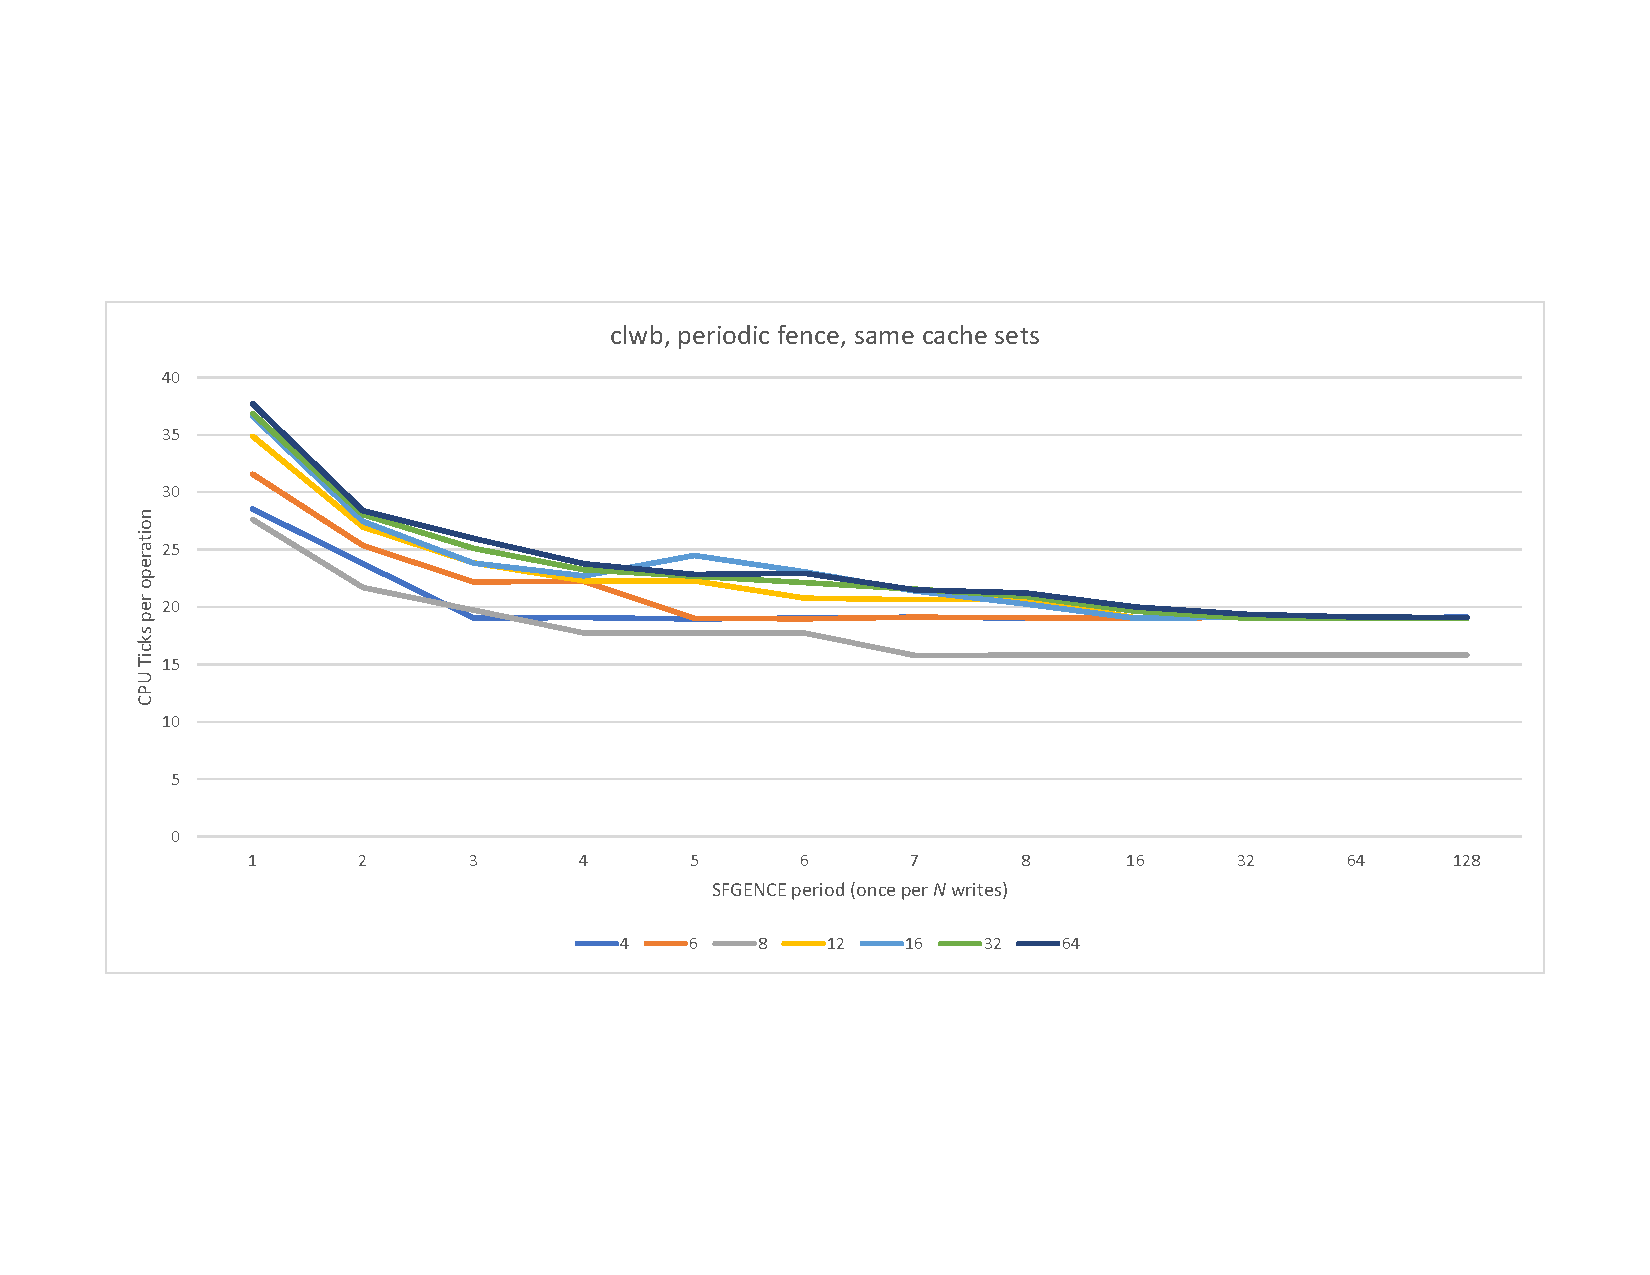
\includegraphics[scale=0.35]{micro/nvm-clwb-periodic-same.pdf}
\end{figure}

\begin{figure}
    \centering
    \caption{NVM Linked List Baseline (No Flush)}\label{micro:llbaseline:noflush}
    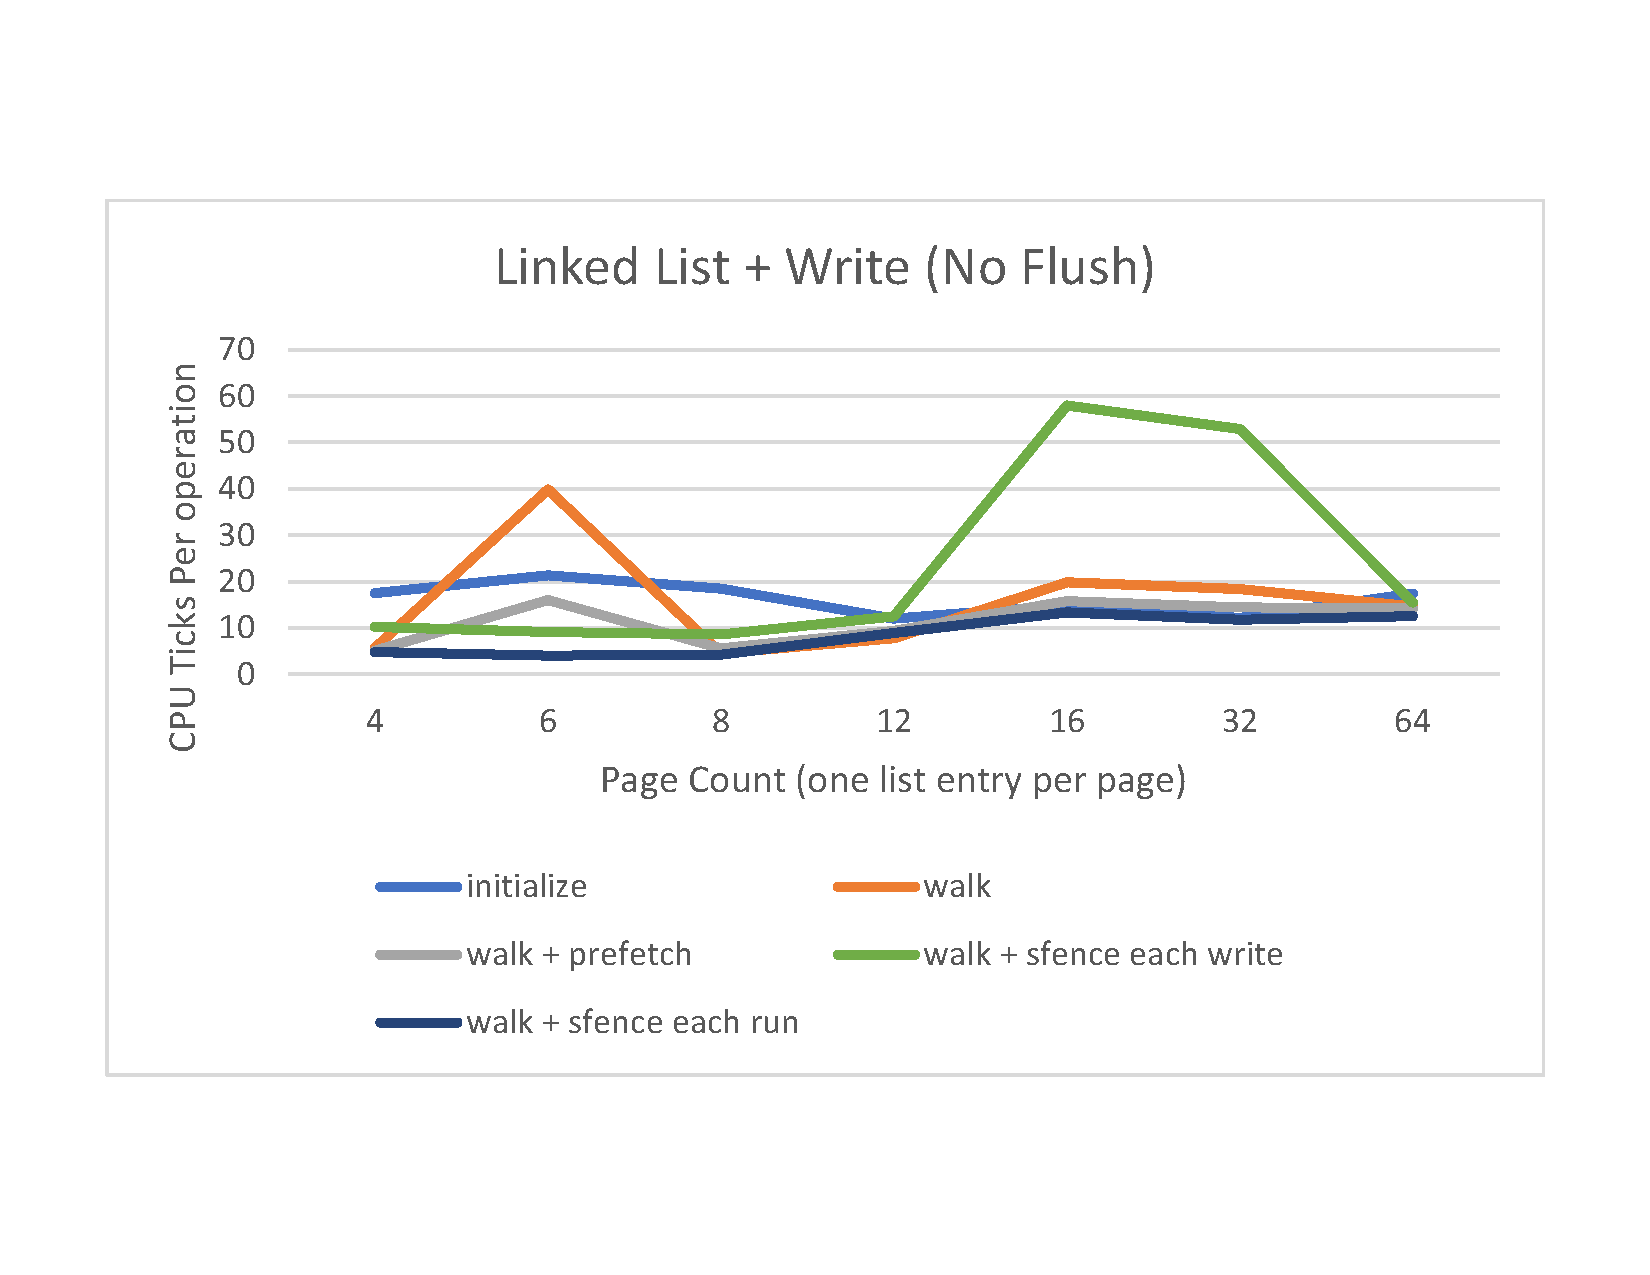
\includegraphics[scale=0.35]{micro/nvm-linked-list-baseline-no-flush.pdf}
\end{figure}

\begin{figure}
    \centering
    \caption{NVM Linked List Baseline (With Flush)}\label{micro:llbaseline:flush}
    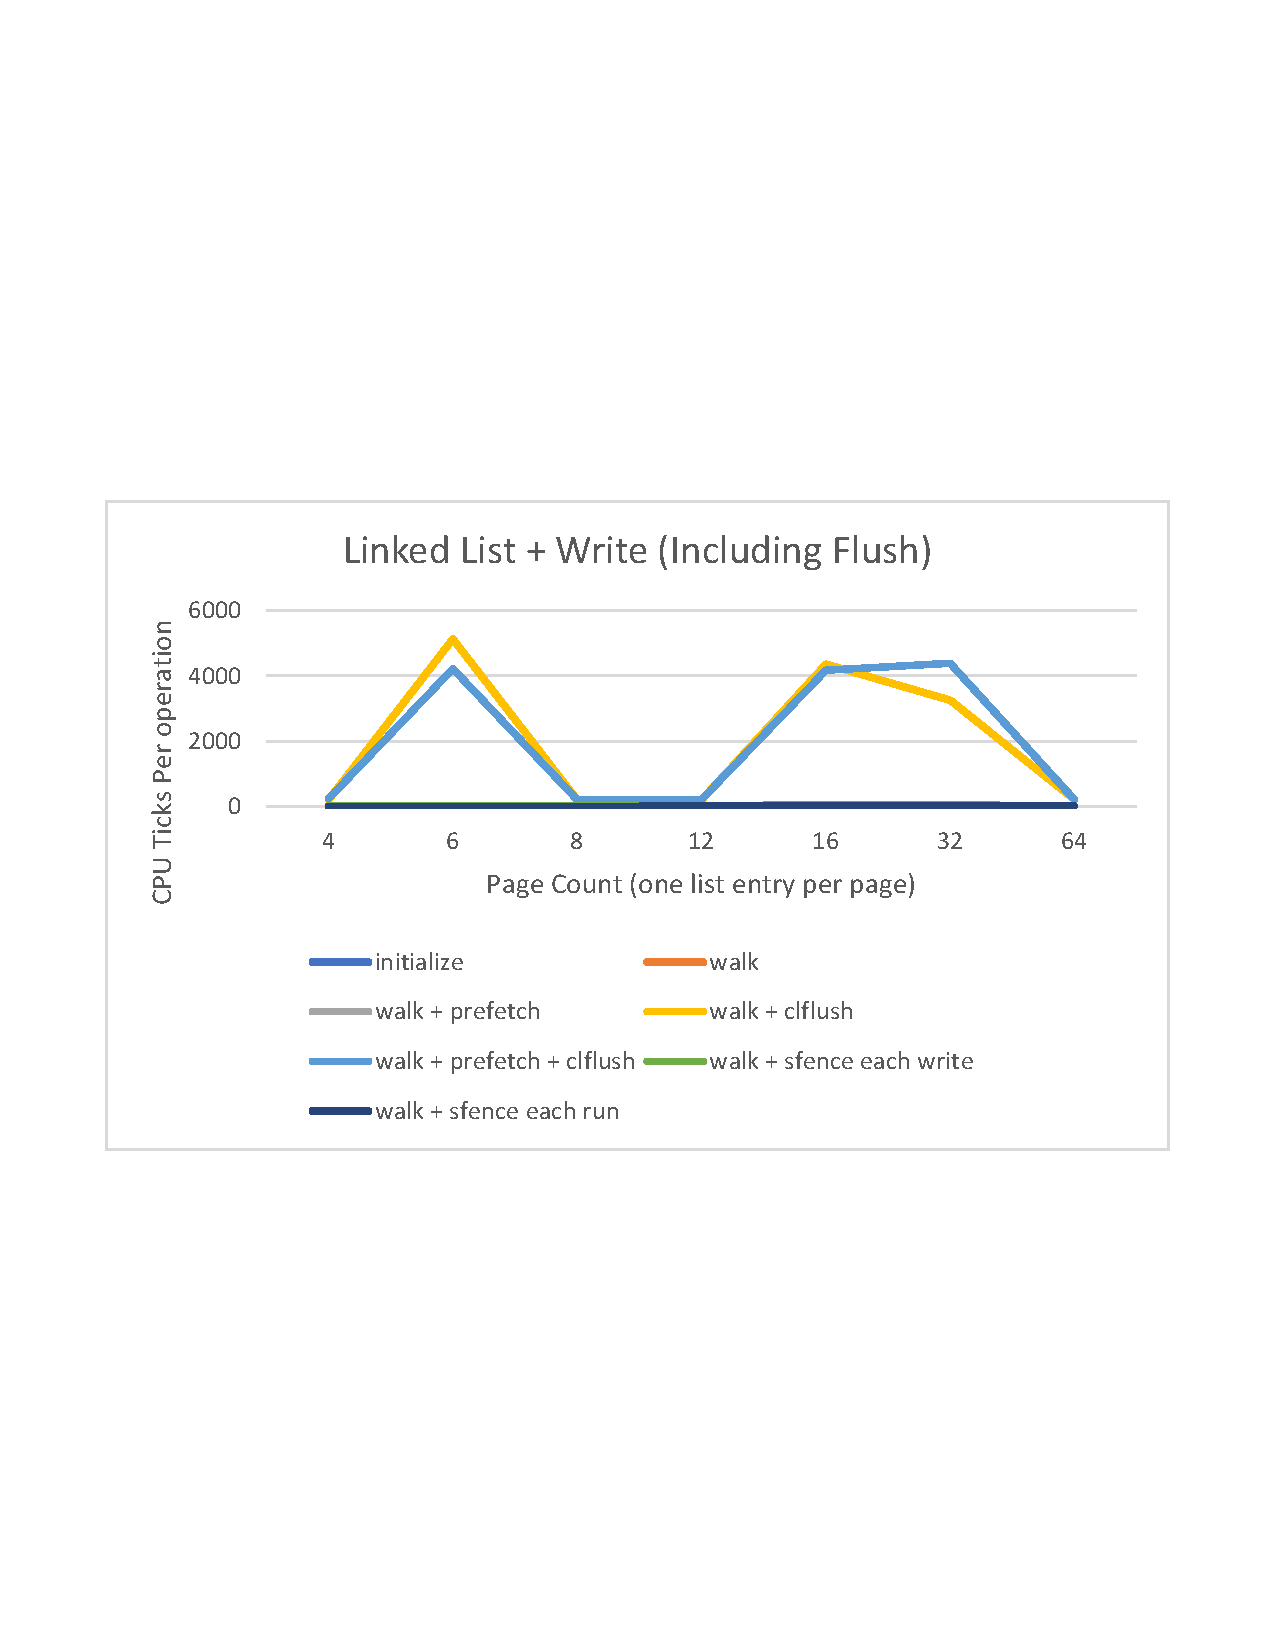
\includegraphics[scale=0.35]{micro/nvm-linked-list-baseline-with-flush.pdf}
\end{figure}

\begin{figure}
    \centering
    \caption{NVM Periodic Fence, No Flush, Different Cache Set}\label{micro:sfence:noflush:different}
    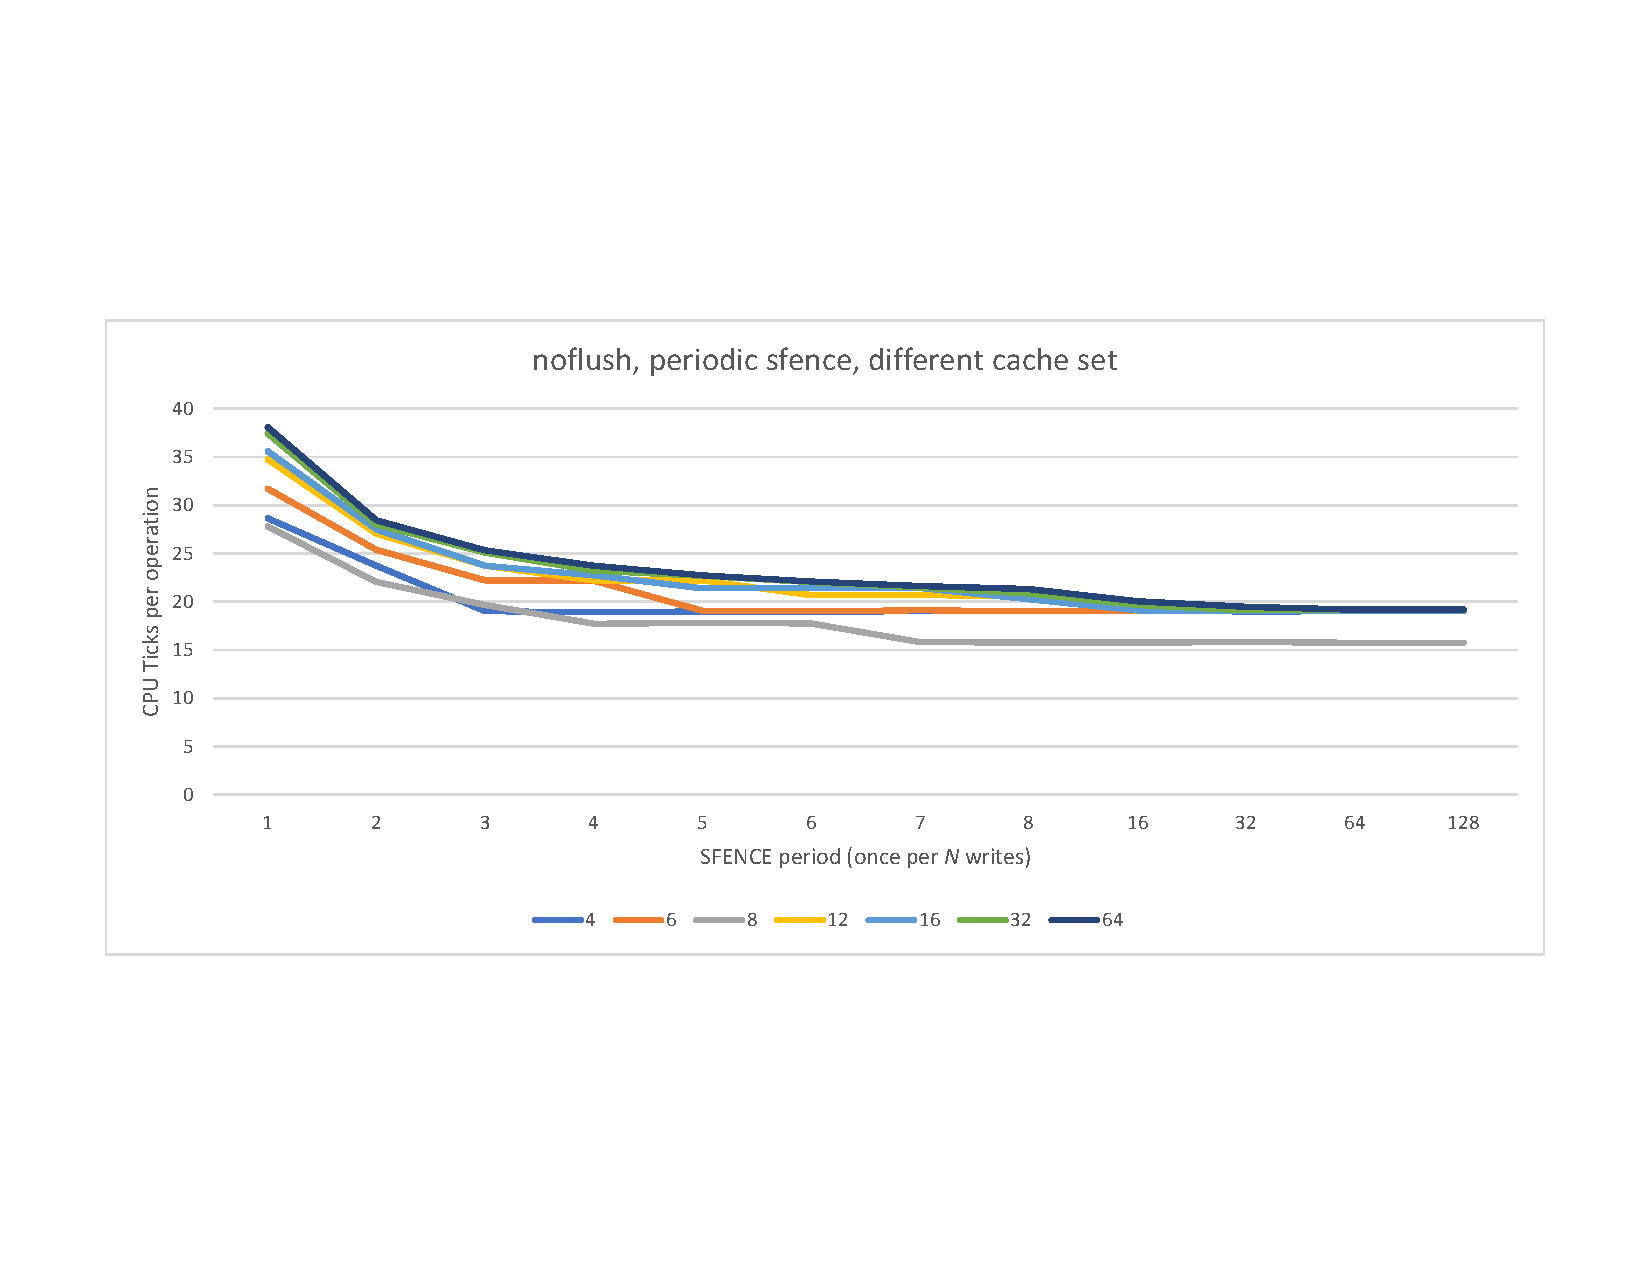
\includegraphics[scale=0.35]{micro/nvm-noflush-periodic-different.pdf}
\end{figure}

\begin{figure}
    \centering
    \caption{NVM Periodic Fence, No Flush, Same Cache Set}\label{micro:sfence:noflush:same}
    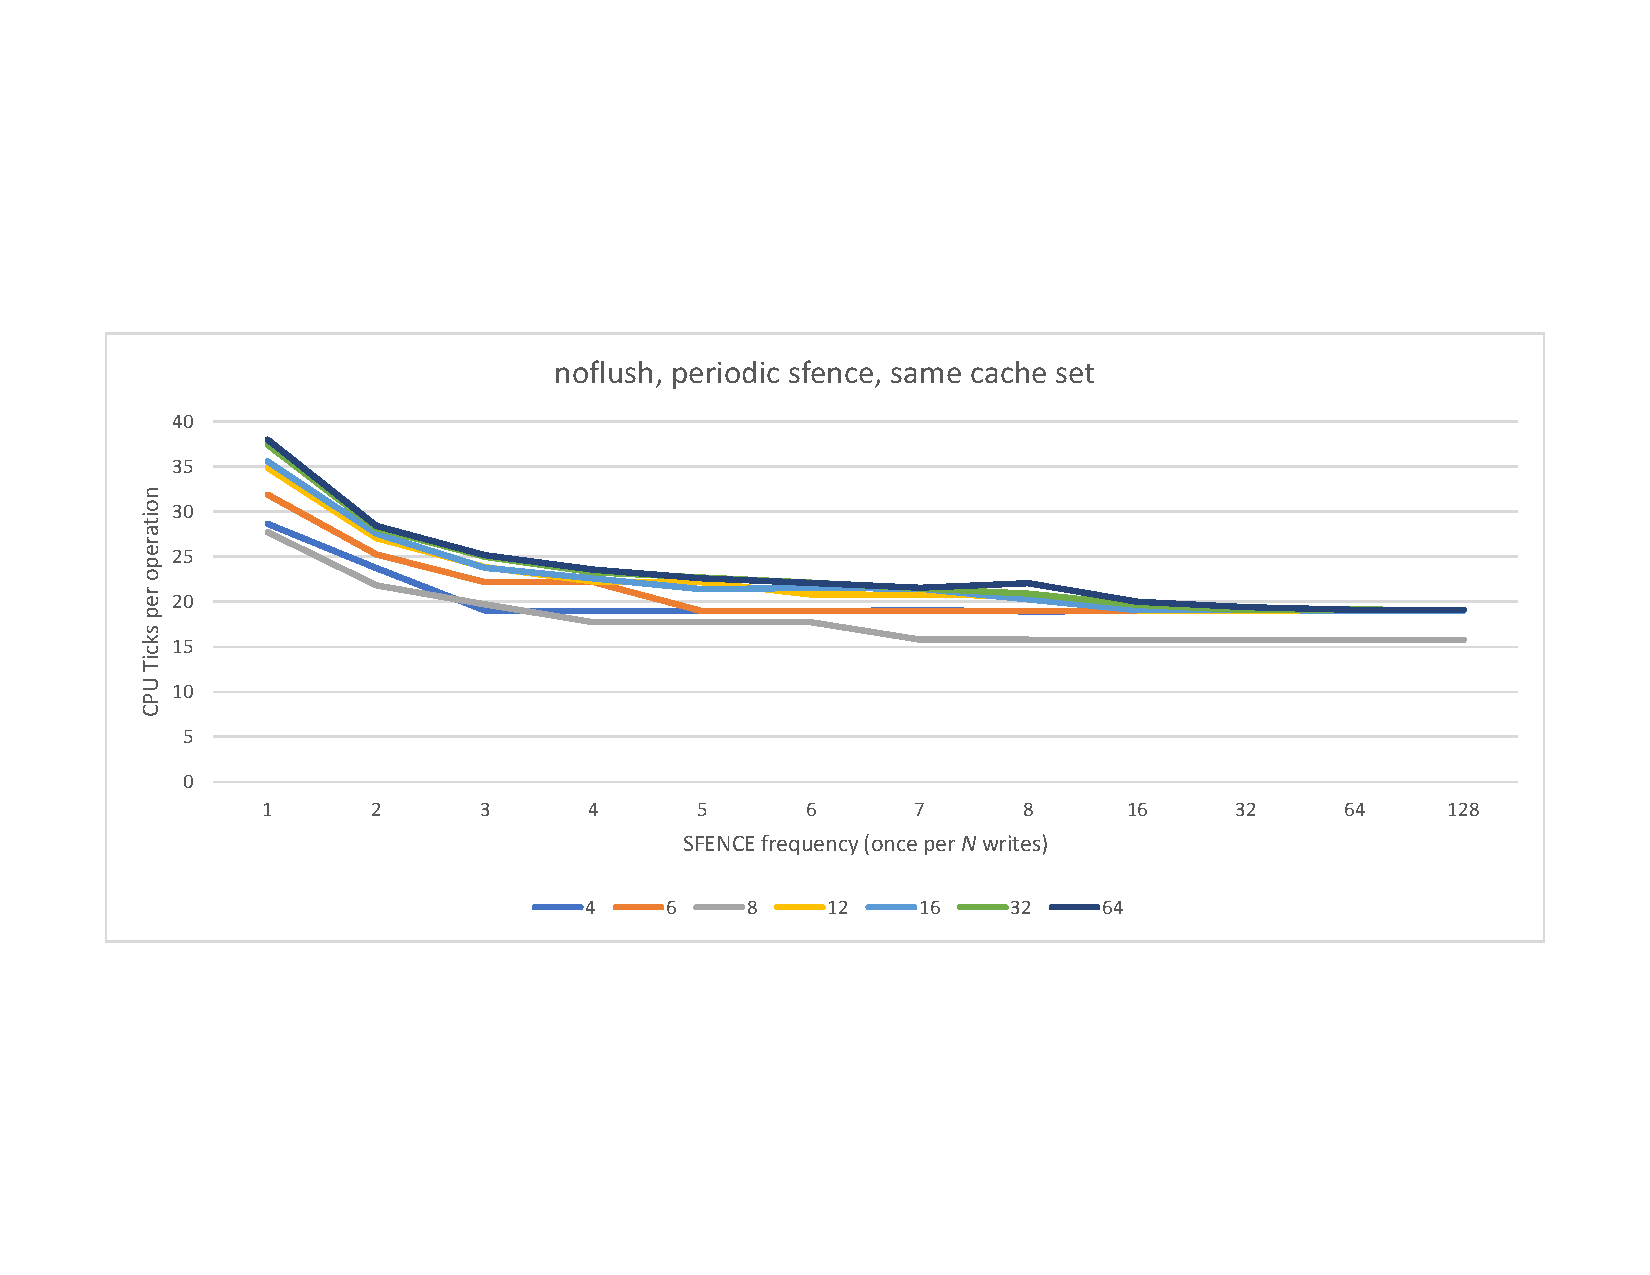
\includegraphics[scale=0.35]{micro/nvm-noflush-periodic-same.pdf}
\end{figure}

\section{Memory Allocator Results}\label{section:results:malloc}

\begin{figure}
    \centering
    \caption{Memory Allocation Tests (Alloc-Free-Alloc)}\label{plot:afa}
    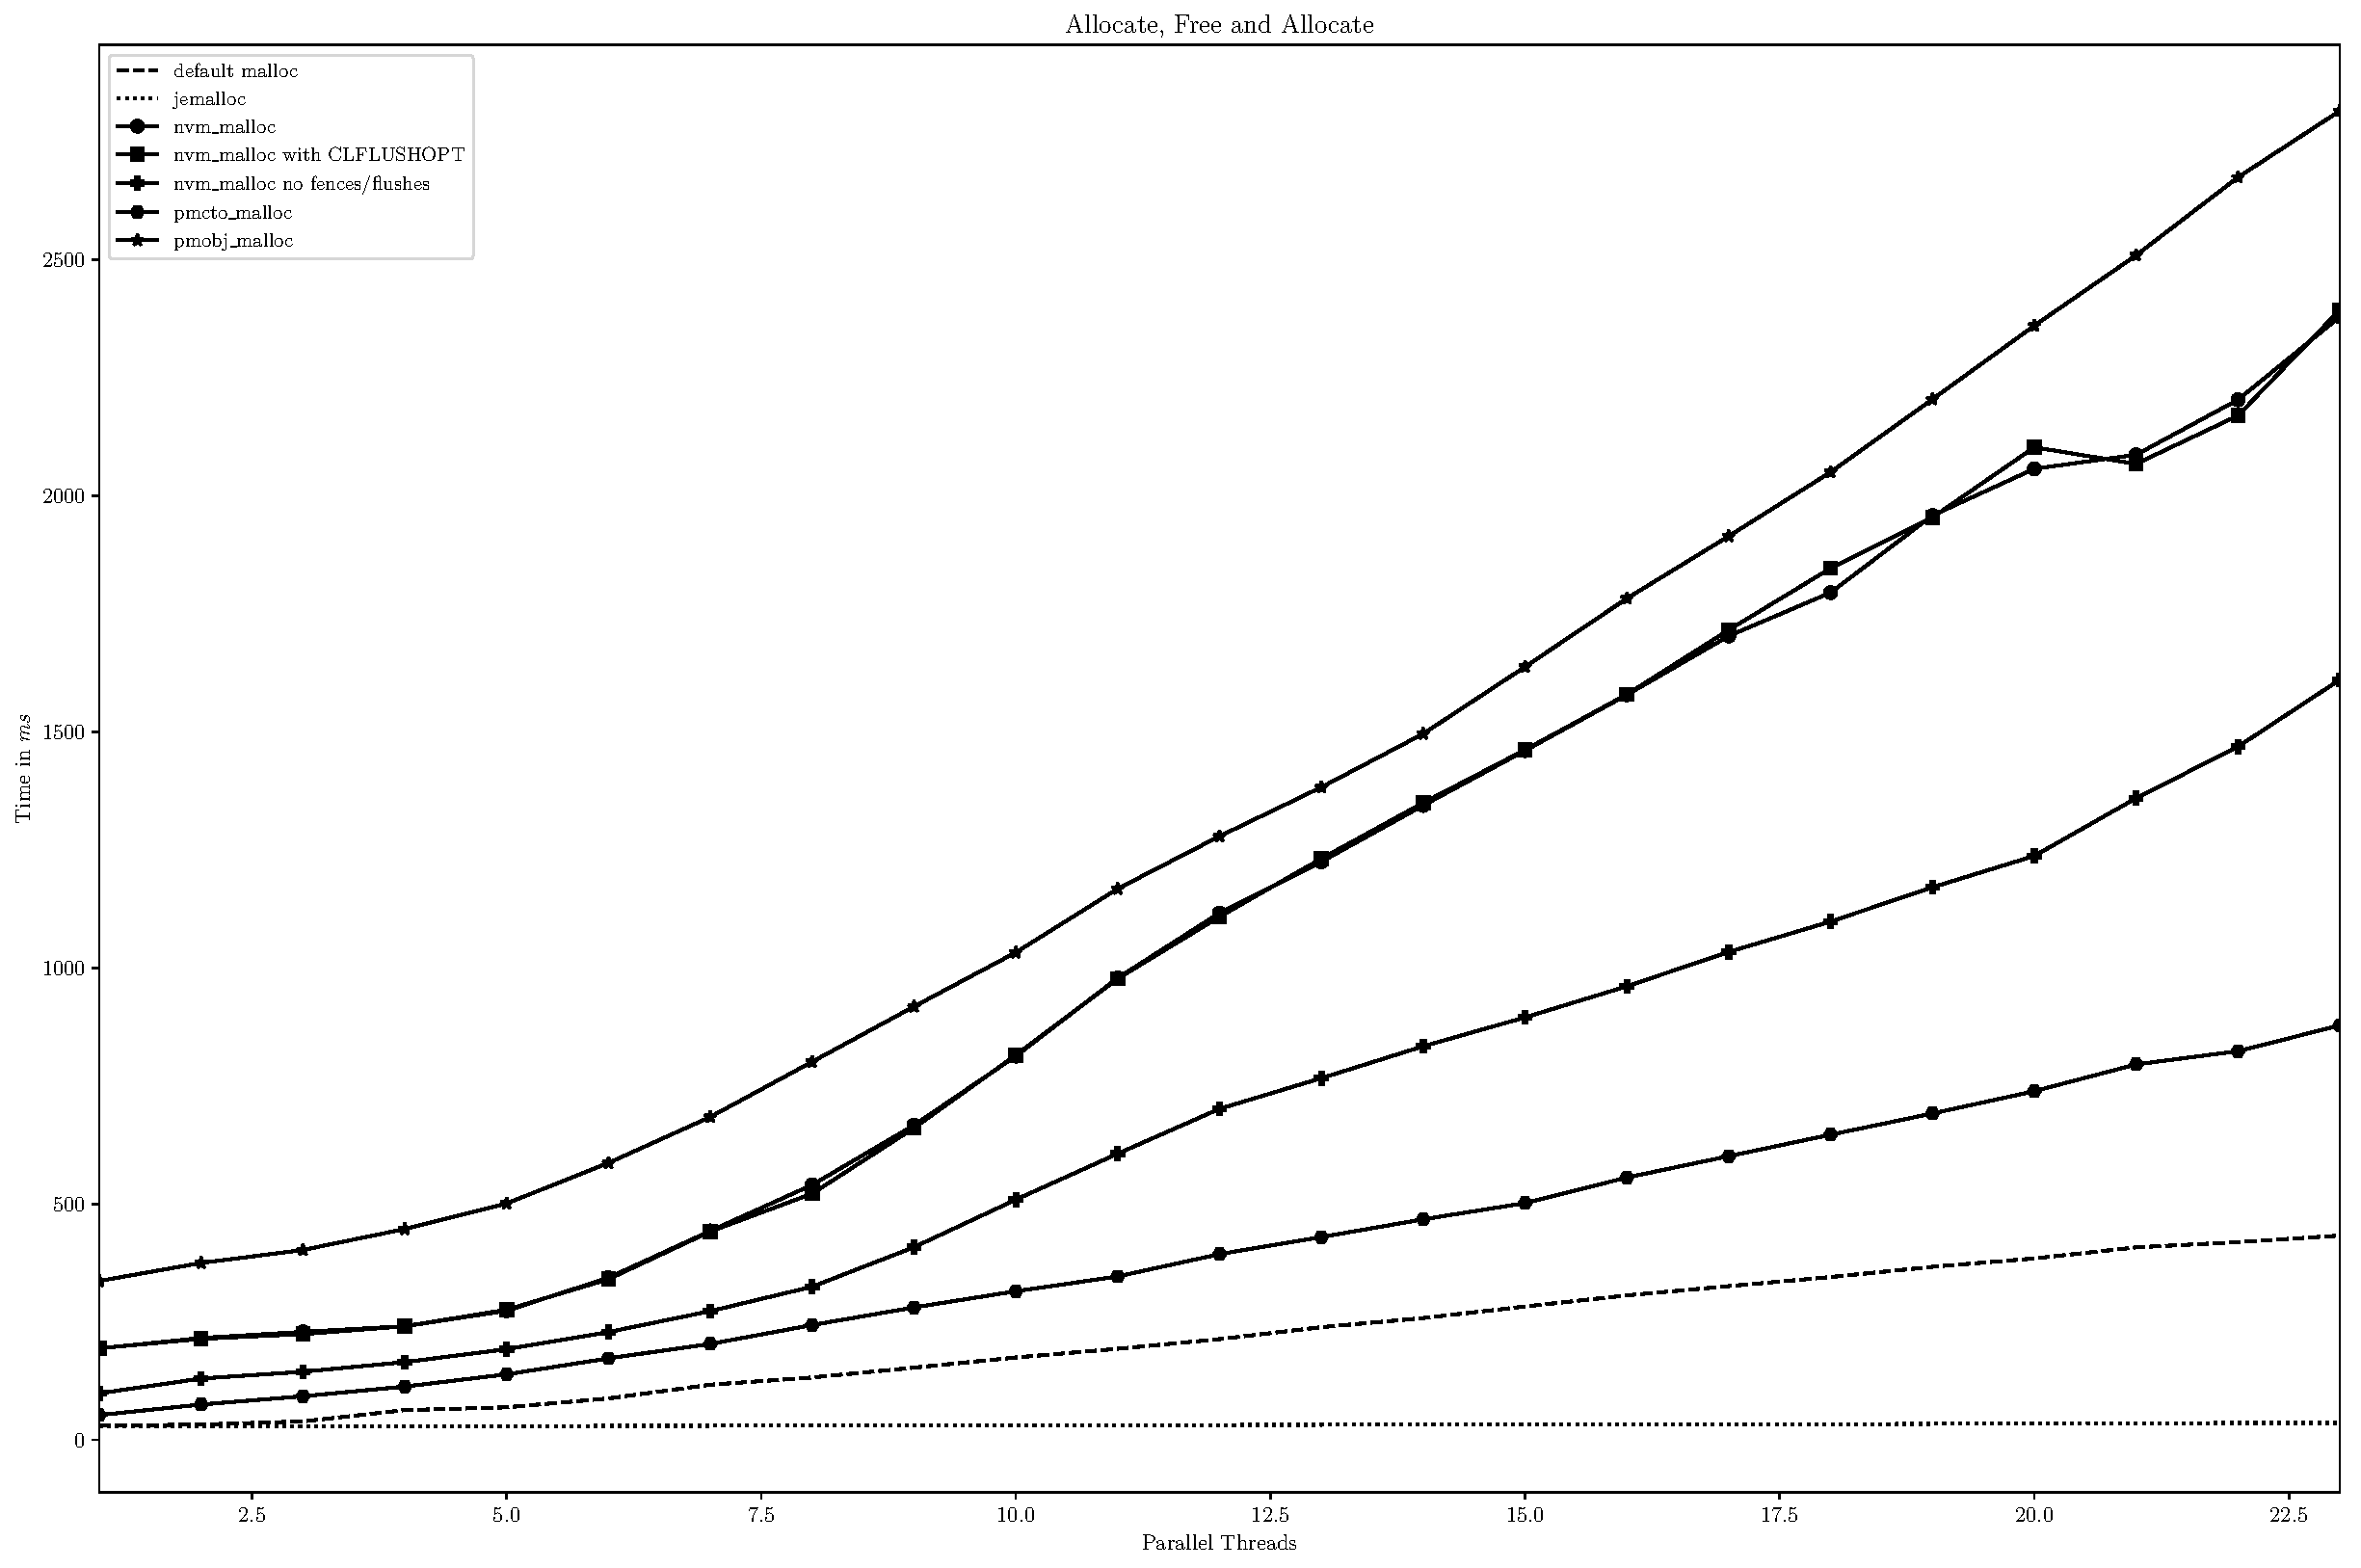
\includegraphics[scale=0.35]{malloc/alloc_free_alloc.pdf}
\end{figure}


\begin{figure}
    \centering
    \caption{Memory Allocation Tests (Alloc-Free)}\label{plot:af}
    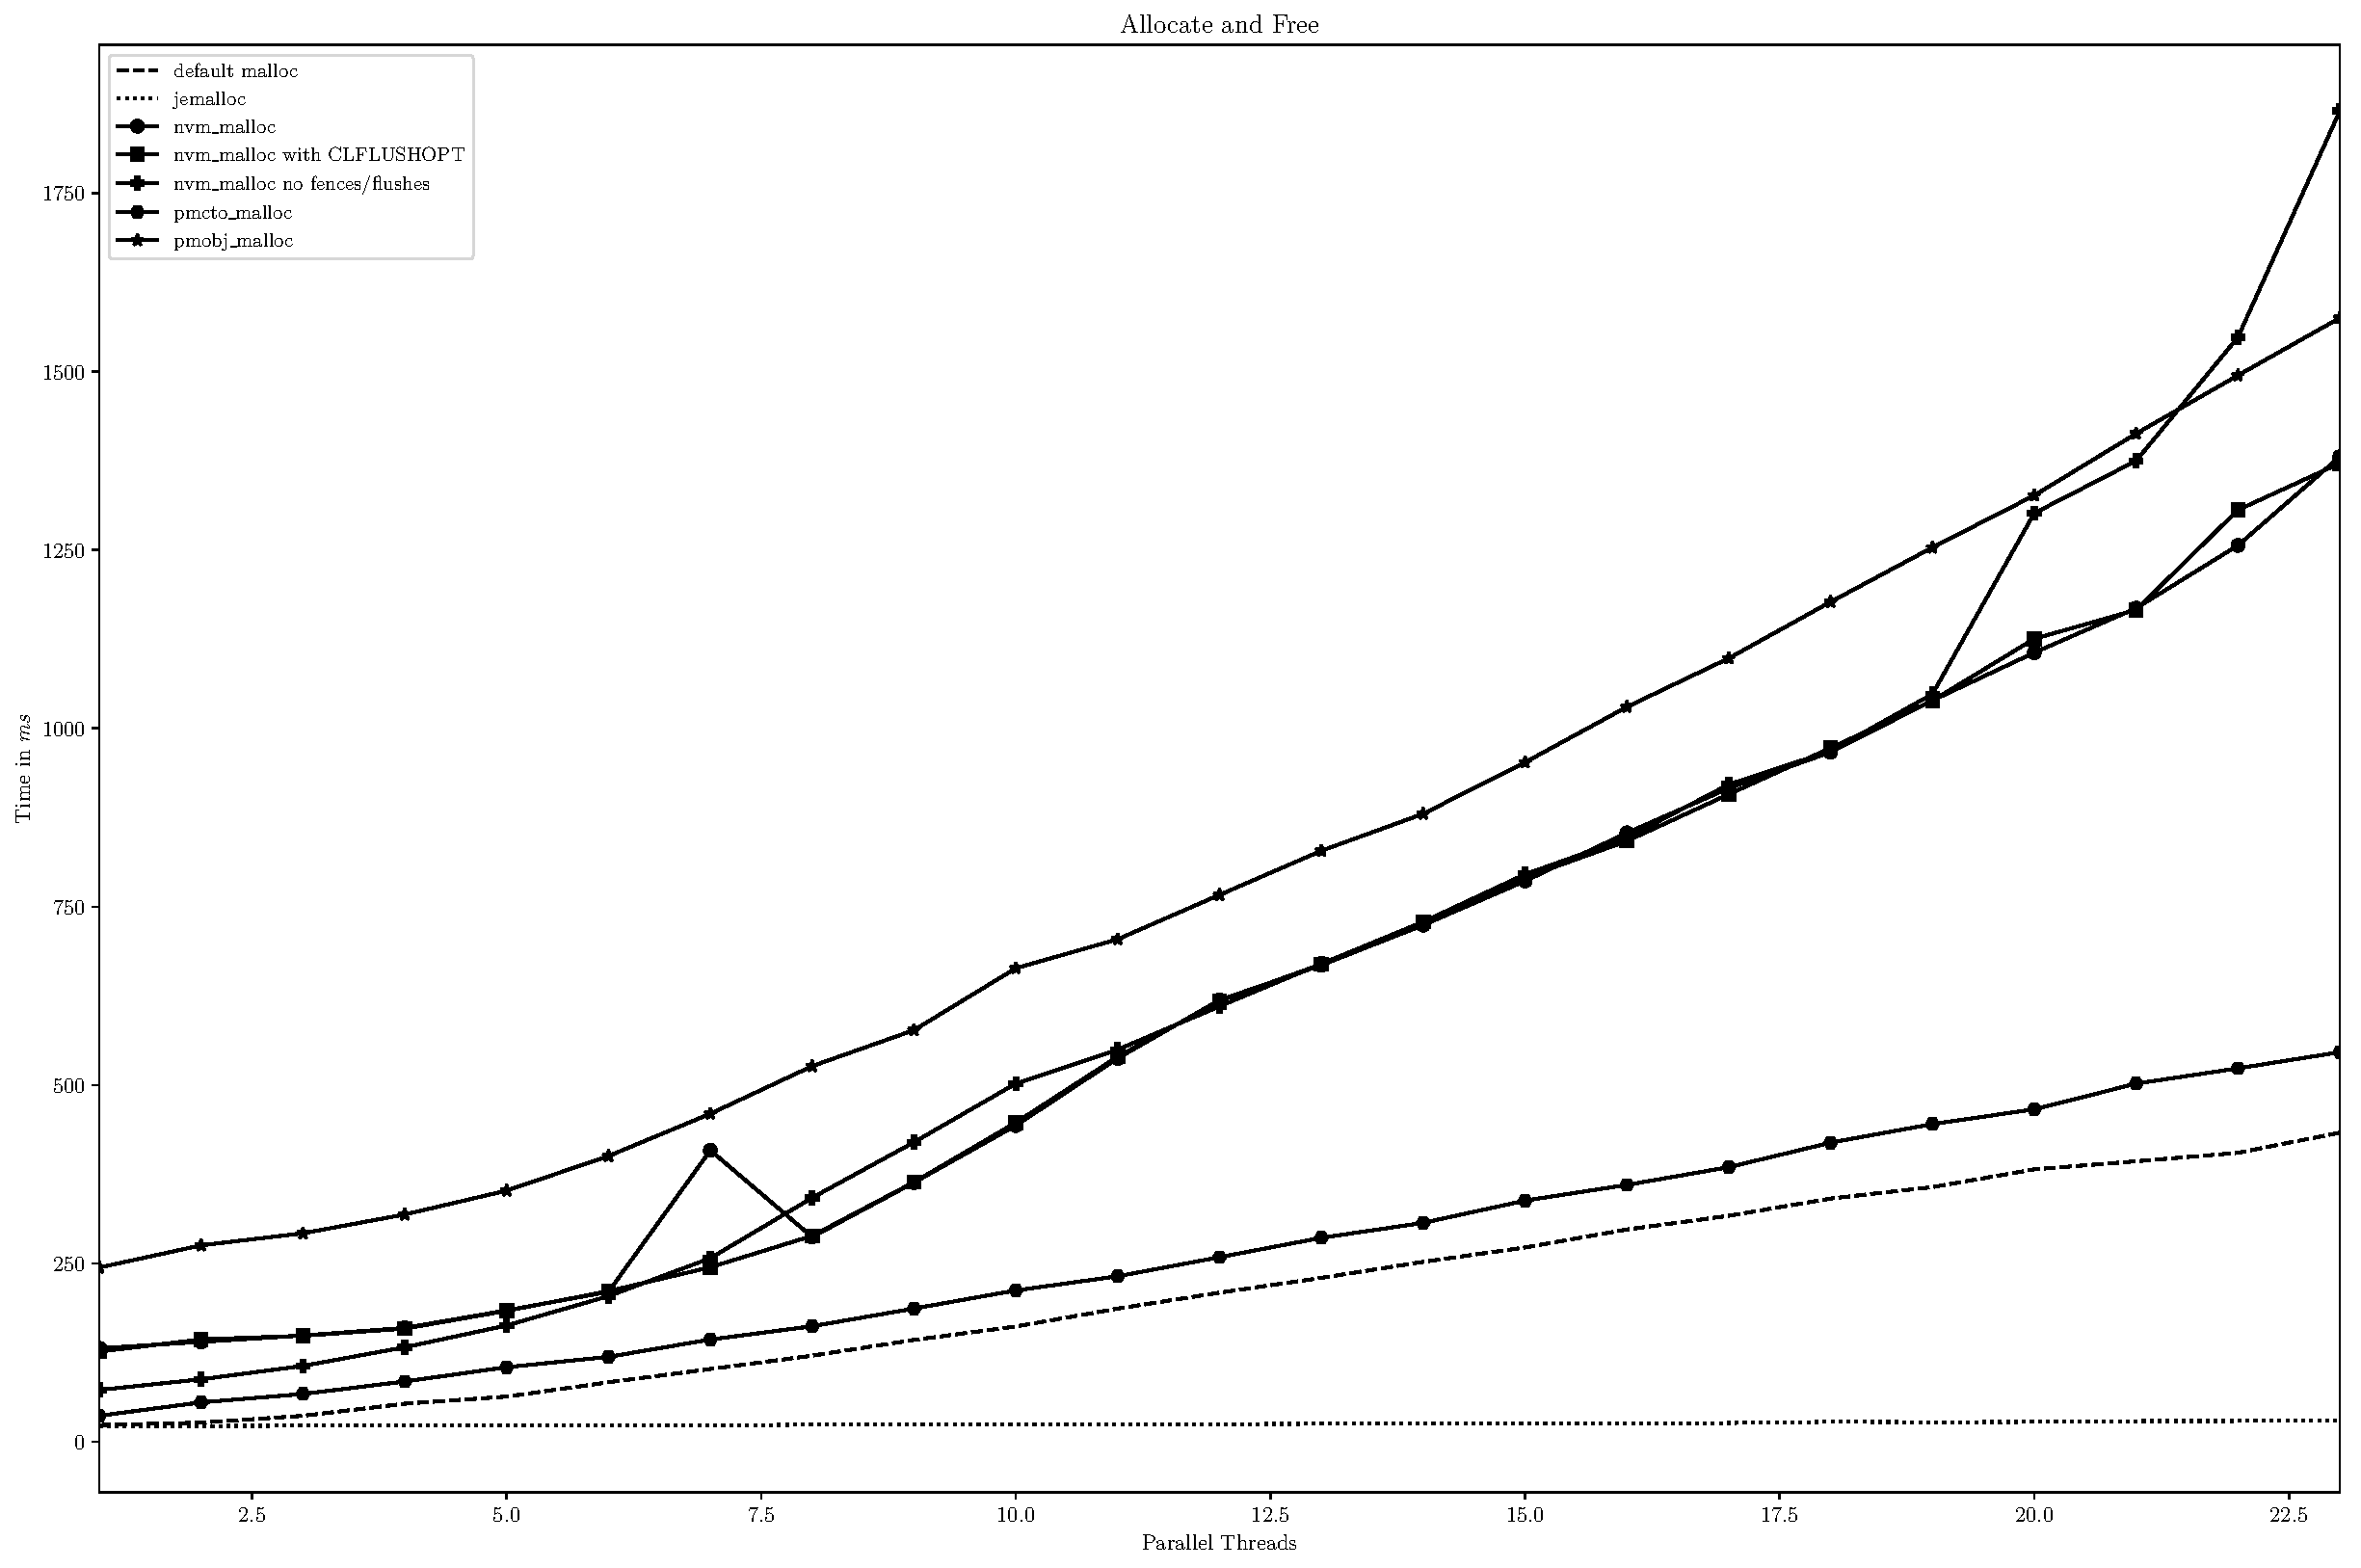
\includegraphics[scale=0.35]{malloc/alloc_free.pdf}
\end{figure}

\begin{figure}
    \centering
    \caption{Memory Allocation Tests (Fastalloc)}\label{plot:fastalloc}
    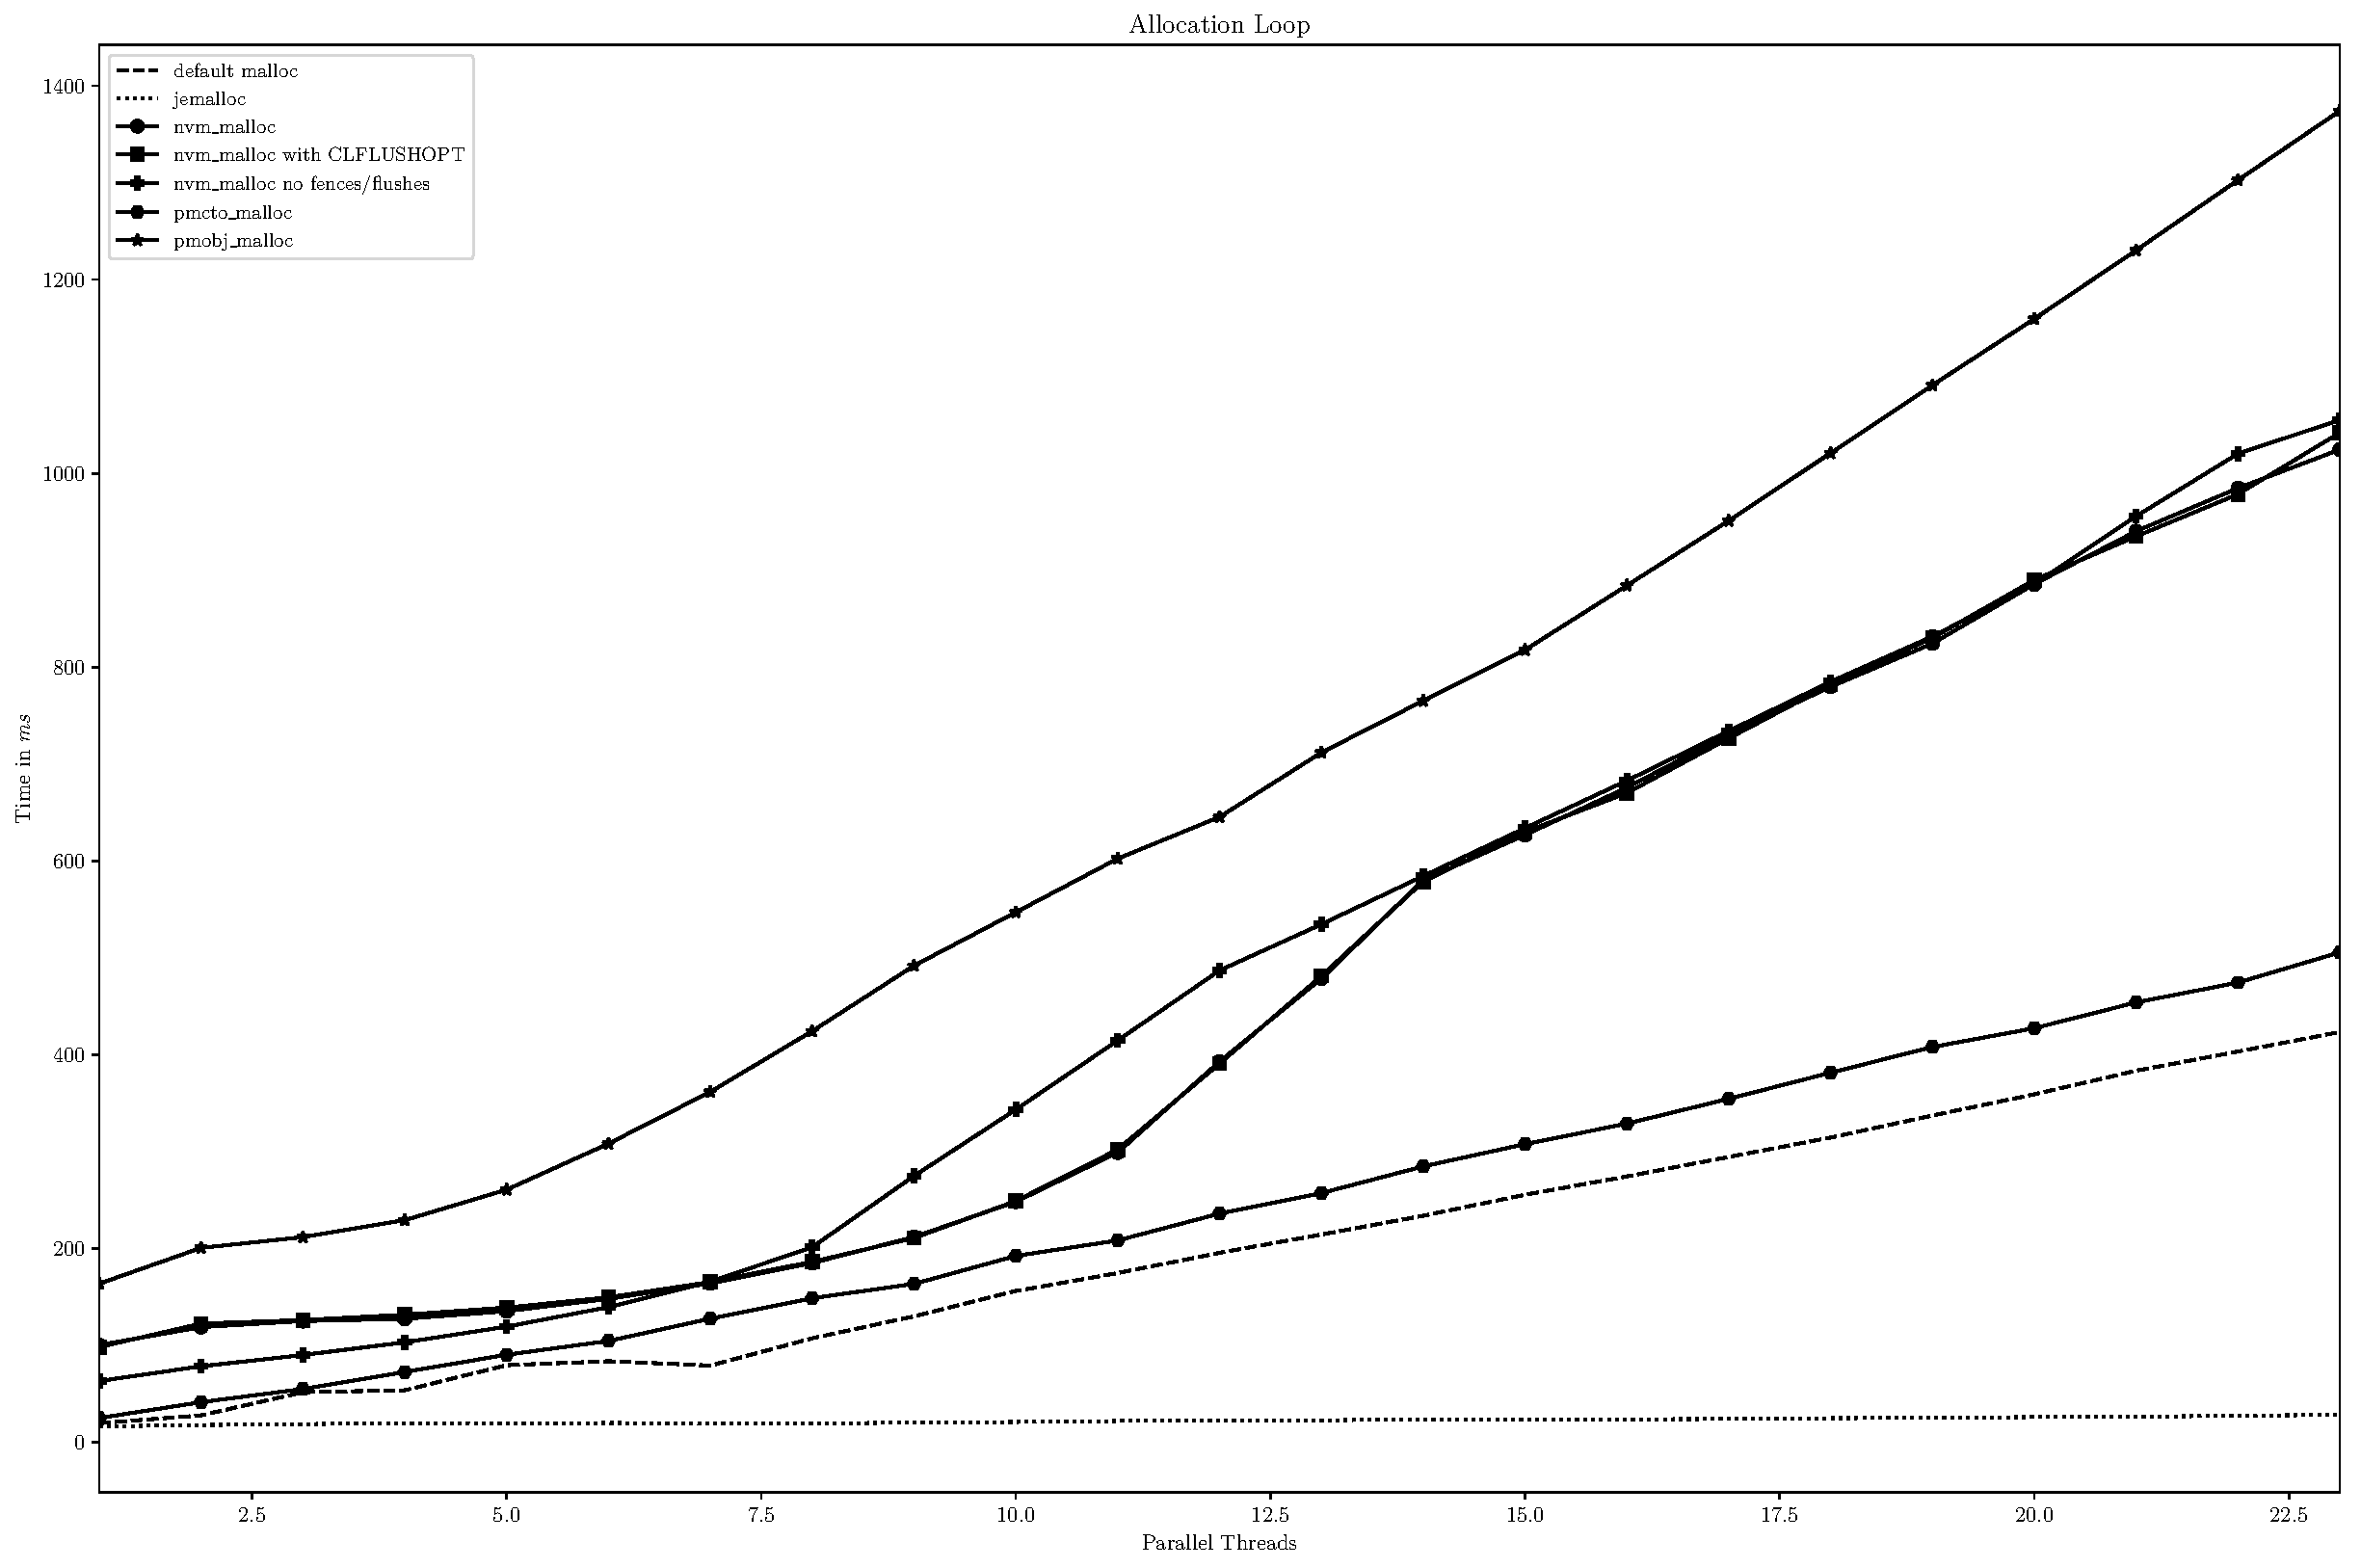
\includegraphics[scale=0.35]{malloc/fastalloc.pdf}
\end{figure}

\begin{figure}
    \centering
    \caption{Memory Allocation Tests (Linkedlist)}\label{plot:linkedlist}
    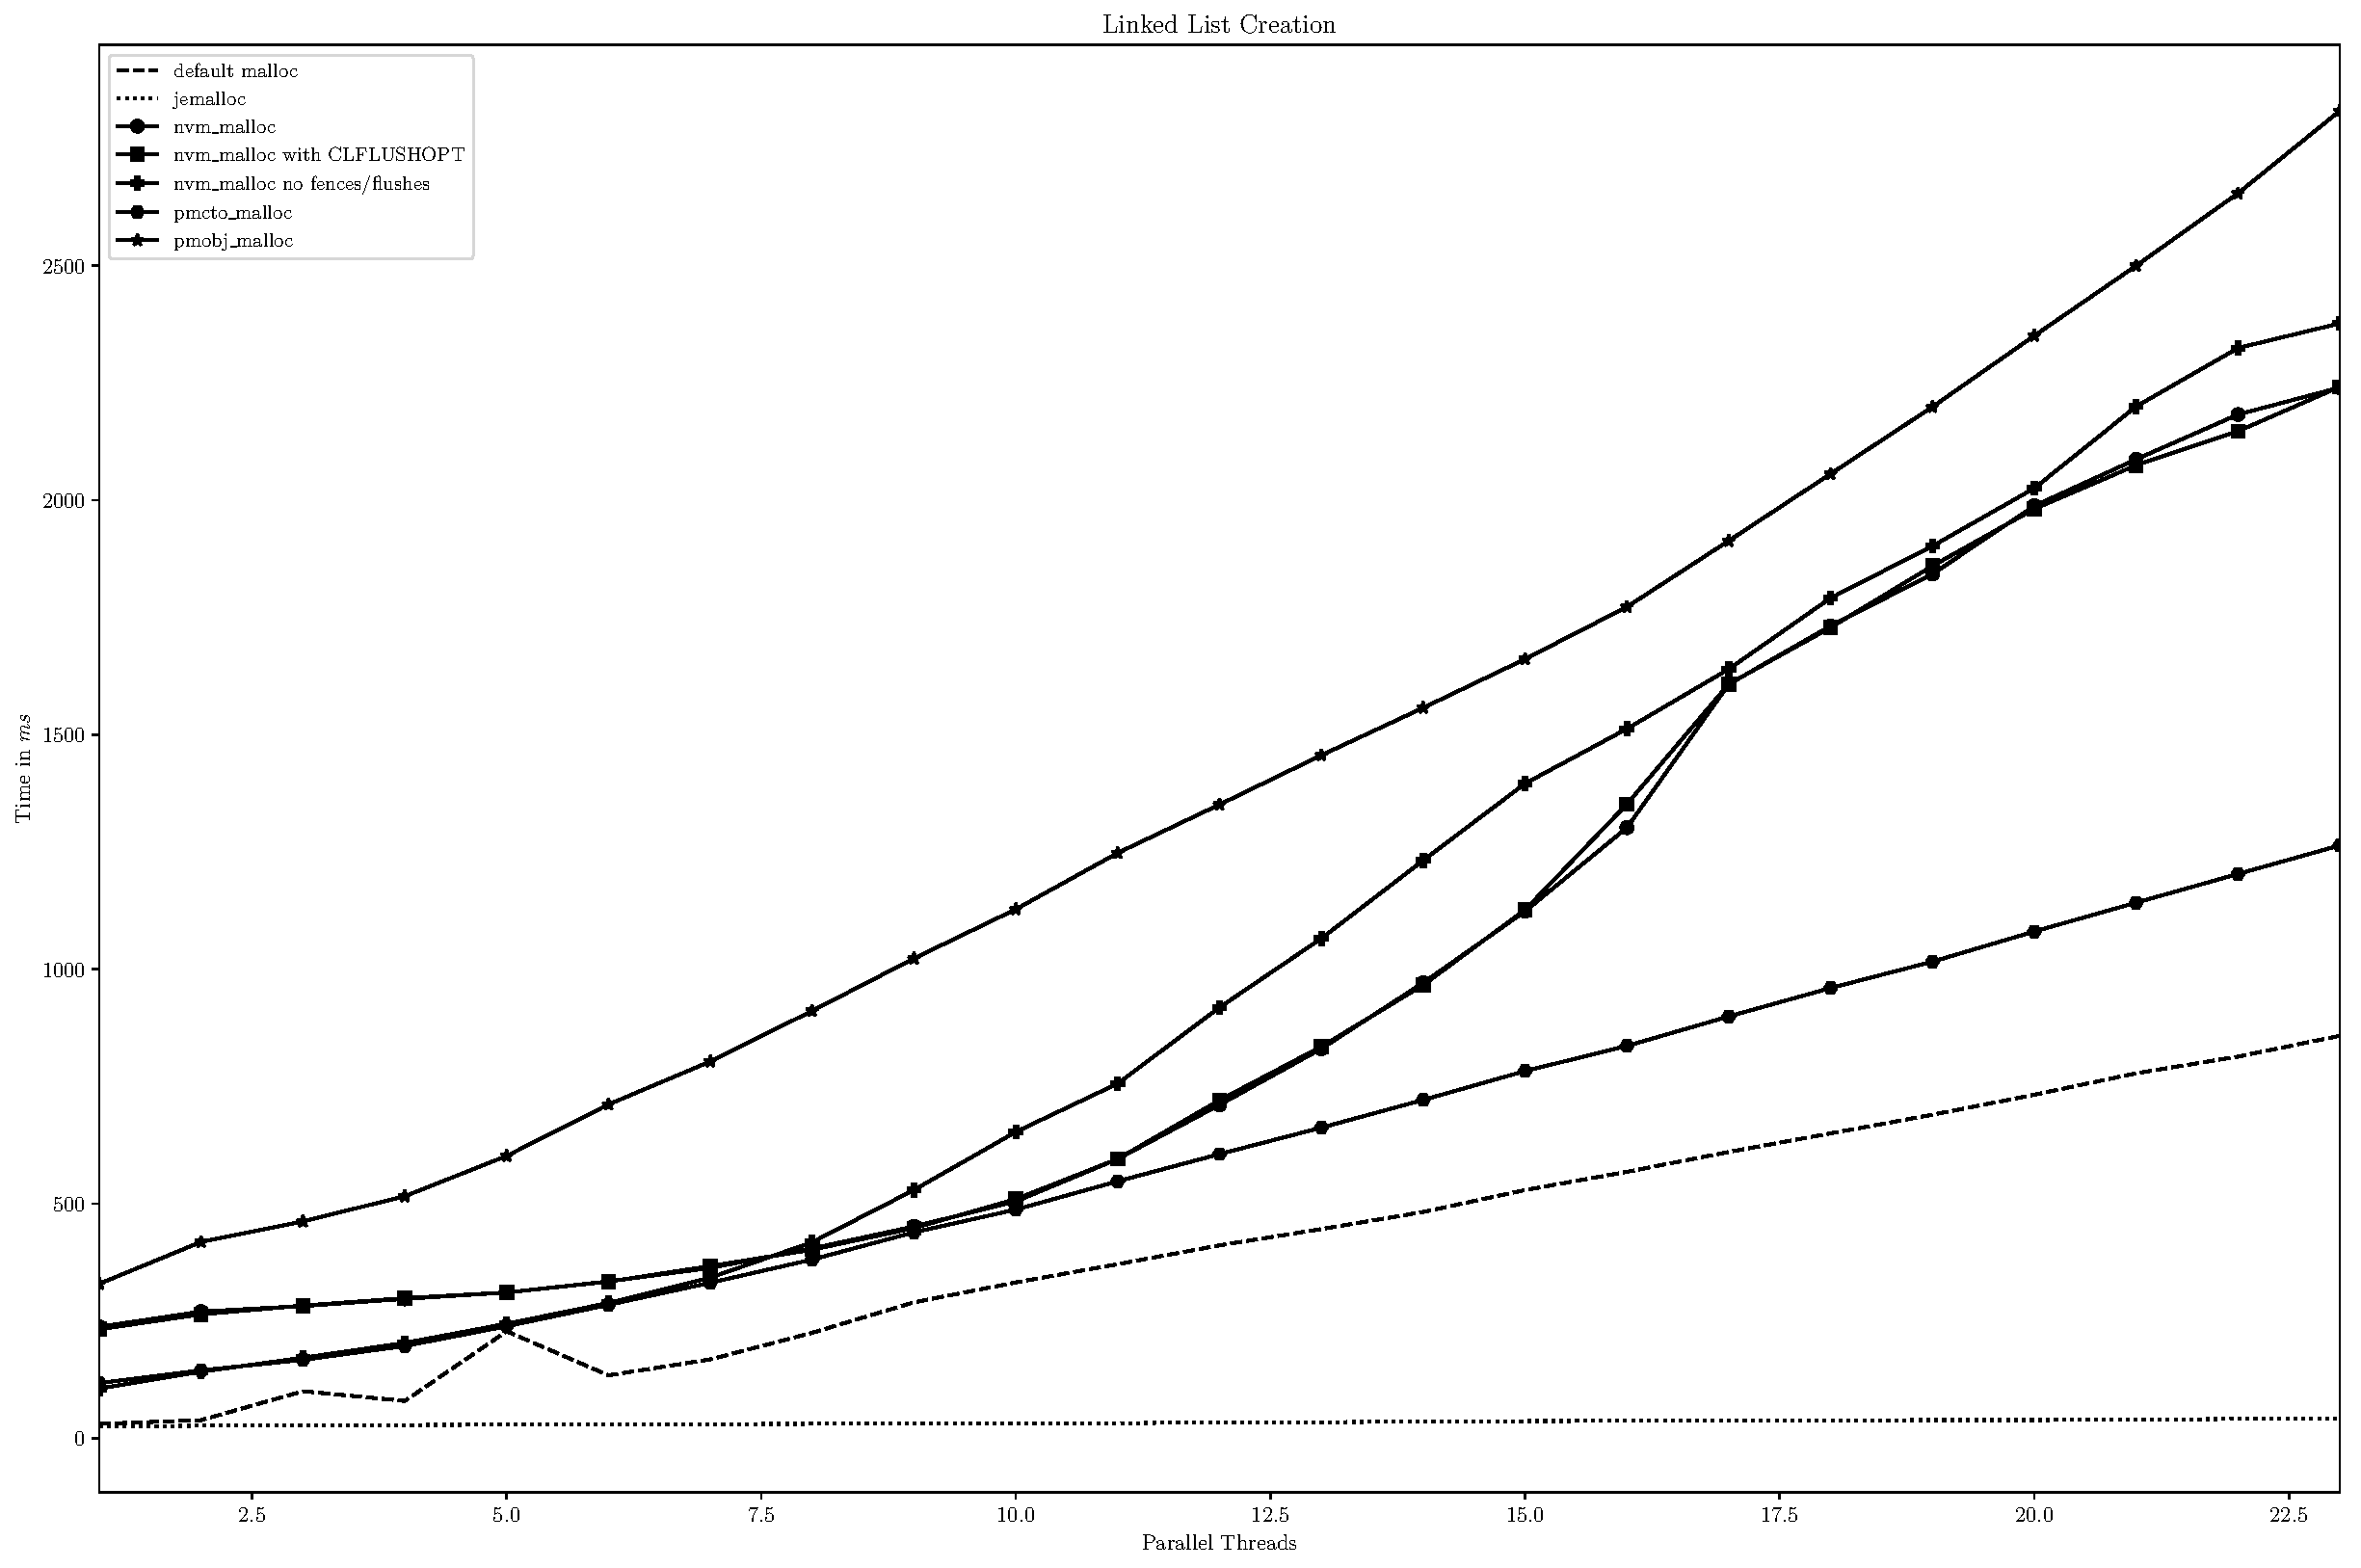
\includegraphics[scale=0.35]{malloc/linkedlist.pdf}
\end{figure}


\endinput



-R read-only load generated, if this is used, -W option should NOT be used 
-Wn where n means
  2  - 2:1 read-write ratio
  3  - 3:1 read-write ratio
  5  - 1:1 read-write ratio
  7  - 2:1 read-Non Temporal Write ratio
  8  - 1:1 read-Non Temporal Write ratio
  10 - 2:1 read-Non Temporal Write ratio (stream triad-like)


dram-baseline-nt-write-same-node.pdf
nt-write-both-nodes.pdf
random-r.pdf
random-W2.pdf
random-W5.pdf
random-w6.pdf
random-W7.pdf
random-W8.pdf
sequential-r.pdf
sequential-w10.pdf
sequential-W2.pdf
sequential-w3.pdf
sequential-W5.pdf
sequential-w6.pdf
sequential-W7.pdf

aep_eval_bandwidth-crop.pdf
aep_eval_idle_latency-crop.pdf
aep_eval_random_read_load_latency-crop.pdf
node-specific-latency-versus-delay-crop.pdf
node-specific-load-data-crop.pdf


%% The following is a directive for TeXShop to indicate the main file
%%!TEX root = report.tex

\chapter{Discussion}
\label{ch:Discussion}



%% The following is a directive for TeXShop to indicate the main file
%%!TEX root = report.tex

\chapter{Conclusions}
\label{ch:Conclusion}

The original goals of this project, as set forth in the proposal were to:

\begin{description}
    \item[Describe a Failure Model] --- I made some progress in this area, as discussed in \S \ref{section:model:failure}.  Thus, this goal has been accomplished at some level.
    \item[Durability] --- much of the micro-benchmark work that I did was exploring the tension between performance and crash durability.  Thus, I would note that this goal has been accomplished at some level.
    \item[Performance Evaluation] --- this goal was to evaluate adding non-volatile memory support to those systems.  No work was done in this space due to resource constraints.  This remains future work.
\end{description}

The \textbf{primary objective} of this project was to demonstrate the ability to conduct 
independent research.  While I have worked with a number of people during this project, including 
discussing preliminary results and possible future directions, the work described in this document 
rests upon the research that I have conducted.  The experimental results in Chapter \ref{ch:Results}
are directly based upon data that I collected.  I wrote the micro-benchmark code, modified the memory allocator benchmark framework, wrote additional scripts to automate running and collecting a vast volume of data.

Thus, I submit to those evaluating my work that this is sufficient to demonstrate the ability to conduct independent research in pursuit of my PhD at The University of British Columbia.
 

%    3. Notes
%    4. Footnotes

%    5. Bibliography
% this is just a big long list of references to ensure the bibliography gets properly populates.

\nocite{volos2011mnemosyne}
\nocite{condit2009better}
\nocite{pelley2014memory}
\nocite{Friedman:2018:PLQ:3178487.3178490} 
\nocite{Memaripour:2017:AIU:3064176.3064215} 
\nocite{Hsu:2017:NPP:3064176.3064204} 
\nocite{Kolli:2017:LP:3140659.3080229} 
\nocite{Kolli:2017:LP:3079856.3080229} 
\nocite{lee2017wort}
\nocite{Nalli:2017:APM:3093315.3037730} 
\nocite{Nalli:2017:APM:3093336.3037730} 
\nocite{Nalli:2017:APM:3093337.3037730} 
\nocite{Nalli:2017:APM:3037697.3037730} 
\nocite{Oukid:2017:MMT:3137628.3137629} 
\nocite{kolli2017architecting}
\nocite{kannan2018designing}
\nocite{Cohen:2017:ELN:3152284.3133891}
\nocite{Pillai:2017:ACC:3141876.3119897} 
\nocite{liu2018hmfs}
\nocite{Maeng:2017:AIE:3152284.3133920} 
\nocite{Chen:2017:ESP:3123939.3124543}
\nocite{liu2017durable}
\nocite{wang2017hardware}
\nocite{sha2018towards}
\nocite{shin2017proteus}
\nocite{wei2017transactional}
\nocite{papagiannis2017iris}
\nocite{zhang2018simpo}
\nocite{arulraj2017build}
\nocite{yu2017redesign}
\nocite{Oukid:2014:SHS:2619228.2619236} 
\nocite{kim2018clfb}
\nocite{wang2018persisting}
\nocite{zhang2017fine}
\nocite{huang2018nvht}
\nocite{nawab2017dali}
\nocite{giles2017continuous}
\nocite{lee2018write}
\nocite{chen2017udorn}
\nocite{oukid2017data}
\nocite{kim2017papyruskv}
\nocite{liu2017librekv}
\nocite{lu2012bloomstore}
\nocite{venkataraman2011consistent}
\nocite{wu2015lsm}
\nocite{hu2015lama}
\nocite{chen2015persistent}
\nocite{wang2014using}
\nocite{arulraj2015let}
\nocite{fan2014cuckoo}
\nocite{joshi2015efficient}
\nocite{marathe2017persistent}

\begin{singlespace}
\raggedright
\bibliographystyle{IEEEtranSN}
%\bibliographystyle{plainnat}
\bibliography{biblio,nvdimm,phd-app-ref,rpe,failure}
\end{singlespace}

\appendix
%    6. Appendices (including copies of all required UBC Research
%       Ethics Board's Certificates of Approval)
%\include{reb-coa}	% pdfpages is useful here
%\chapter{Supporting Materials}

There was a considerable amount of data collected, only some of which was used.  I'll try to capture
data that I did consider, but did not include in the main text.




\backmatter
%    7. Index
% See the makeindex package: the following page provides a quick overview
% <http://www.image.ufl.edu/help/latex/latex_indexes.shtml>
% Broken link

\end{document}
